
\section{3 lepton training for bump search testing}


To better accertain and map the usefulness of the regular and variational autoencoder in the search for 
new physics, two MonteCarlo signals were used. They both are 3 lep +$e_T^{miss}$ final state SUSY signals,
and thus are fit to use for testing. What we are then looking for are two things. First, we want to see if
there are a resonance in the trilepton mass. Secondly we want to do a bump search of the significance 
in the signal region, and compare the significance with a base test of just eyeballing the $e_T^{miss}$. 
That way, we can get an idea if the method has promise in usage for plublications at the LHC with the ATLAS collaboration. 

\subsubsection*{Regular autoencoder output}

Below are the reconstruction error distributions for the two signals for both the shallow and deep 
regular autoencoder.

\begin{figure}[H]
    \centering
    \begin{subfigure}{.45\textwidth}
        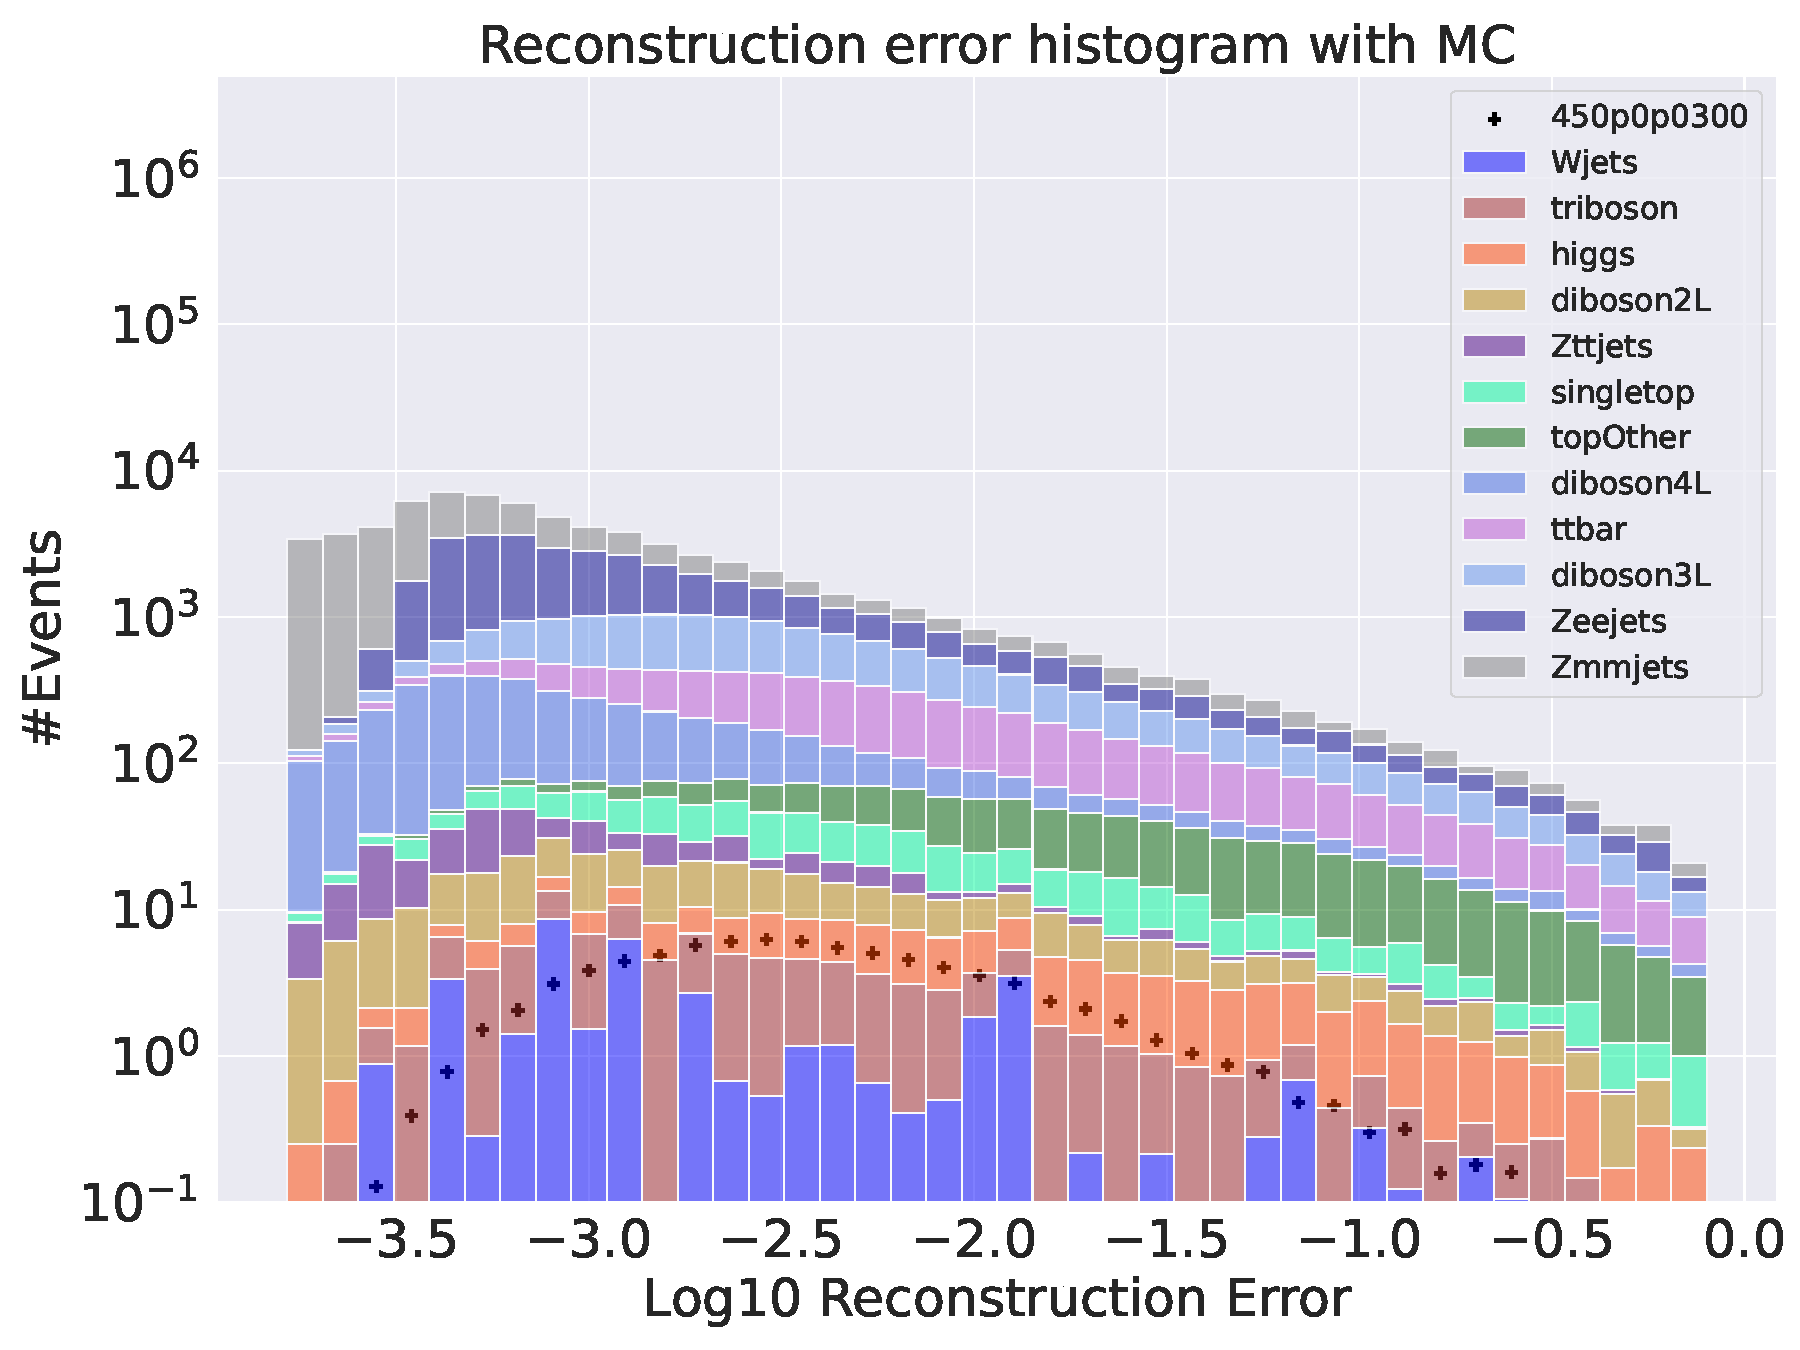
\includegraphics[width=\textwidth]{Figures/AE_testing/big/3lep/b_data_recon_big_rm3_feats_sig_450p0p0300.pdf}
        \caption{ }
        \label{fig:AE_3lep_big_450}
    \end{subfigure}
    \hfill
    \begin{subfigure}{.45\textwidth}
        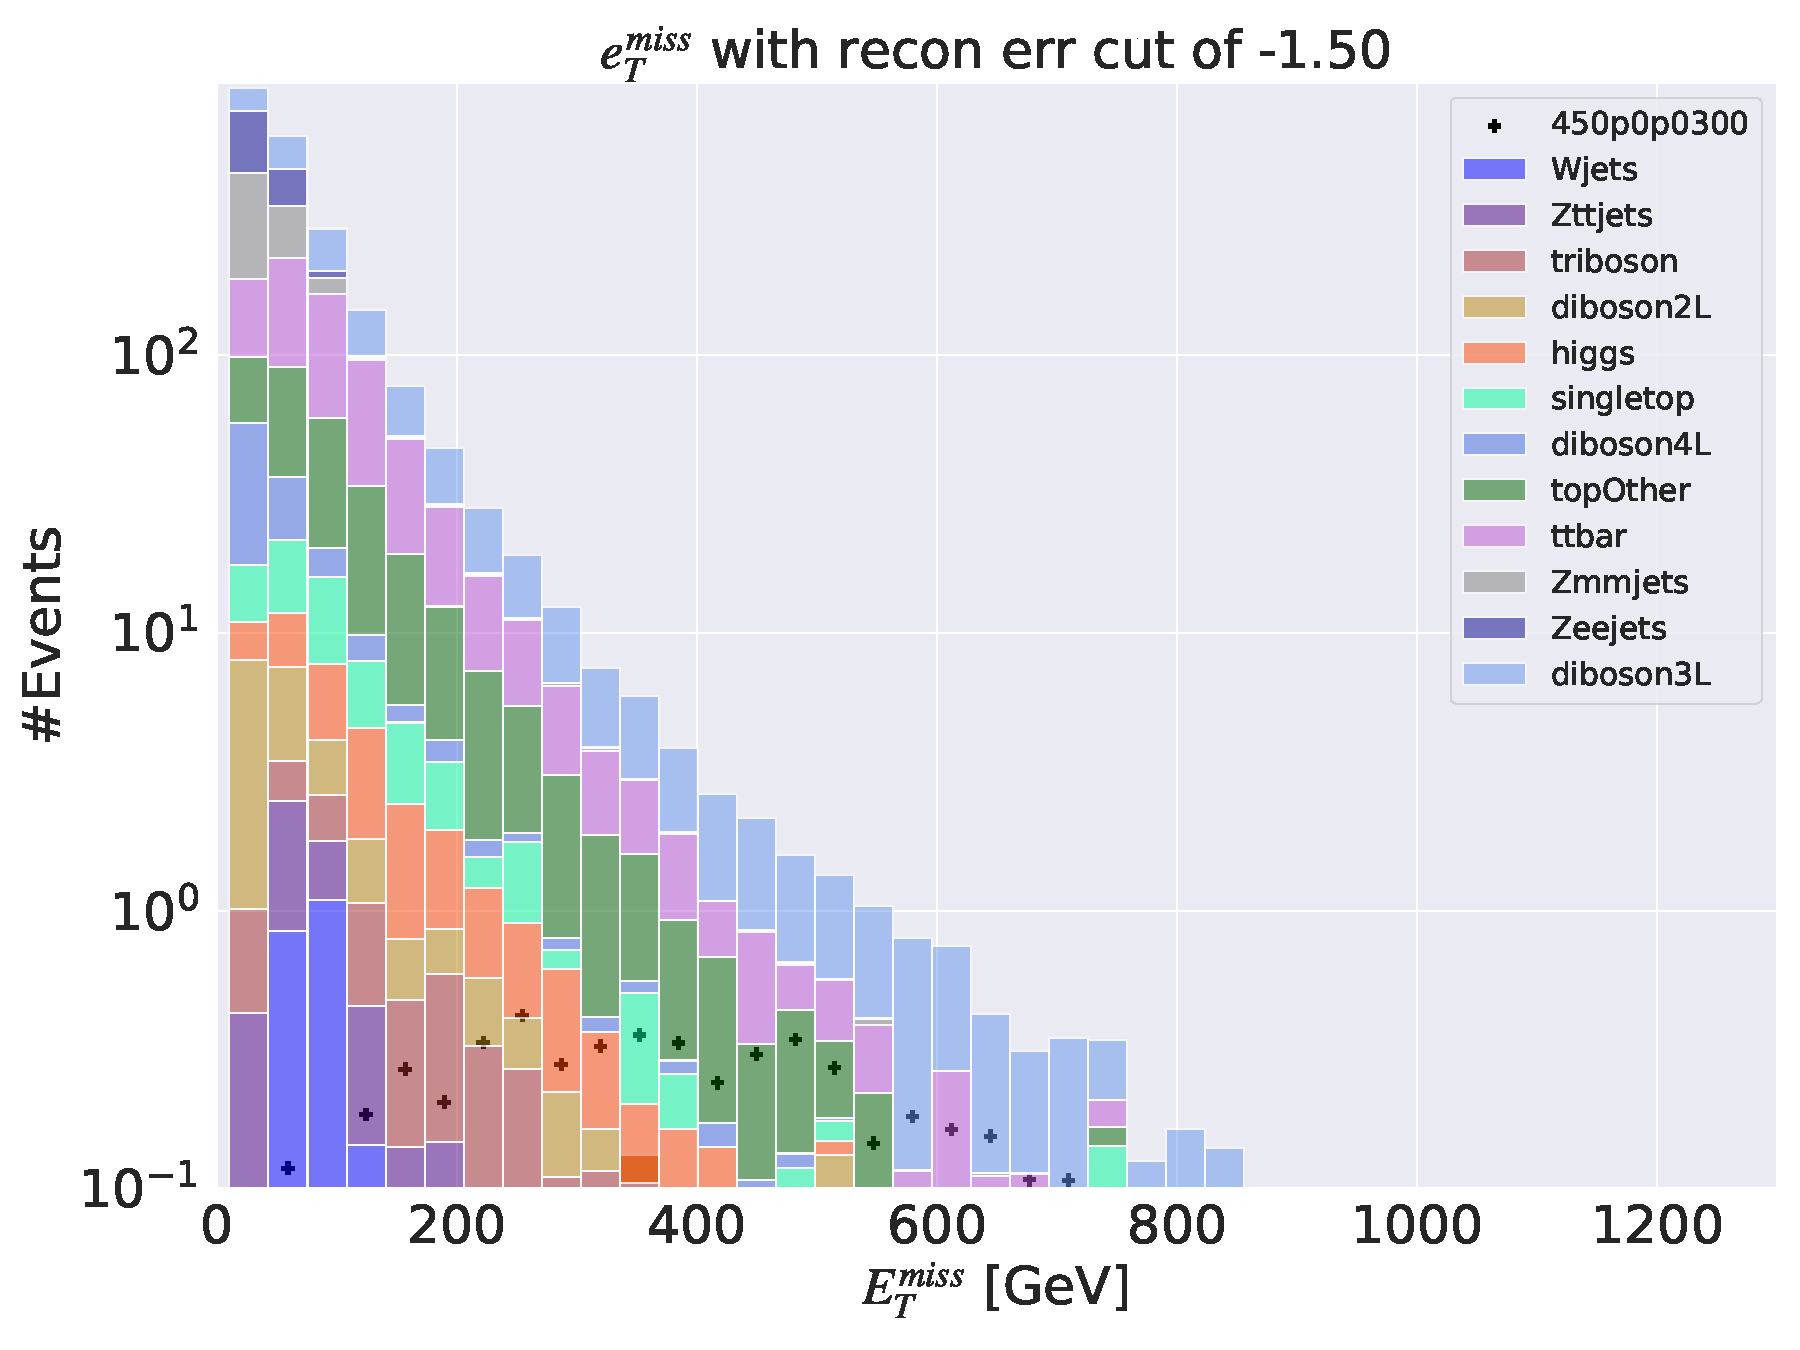
\includegraphics[width=\textwidth]{Figures/AE_testing/big/3lep/b_data_recon_big_rm3_feats_sig_450p0p0300_etmiss_recon_errcut_-1.50.pdf}
        \caption{}
        \label{fig:AE_3lep_big_etmiss_450}
    \end{subfigure}
    \hfill
    \begin{subfigure}{.45\textwidth}
        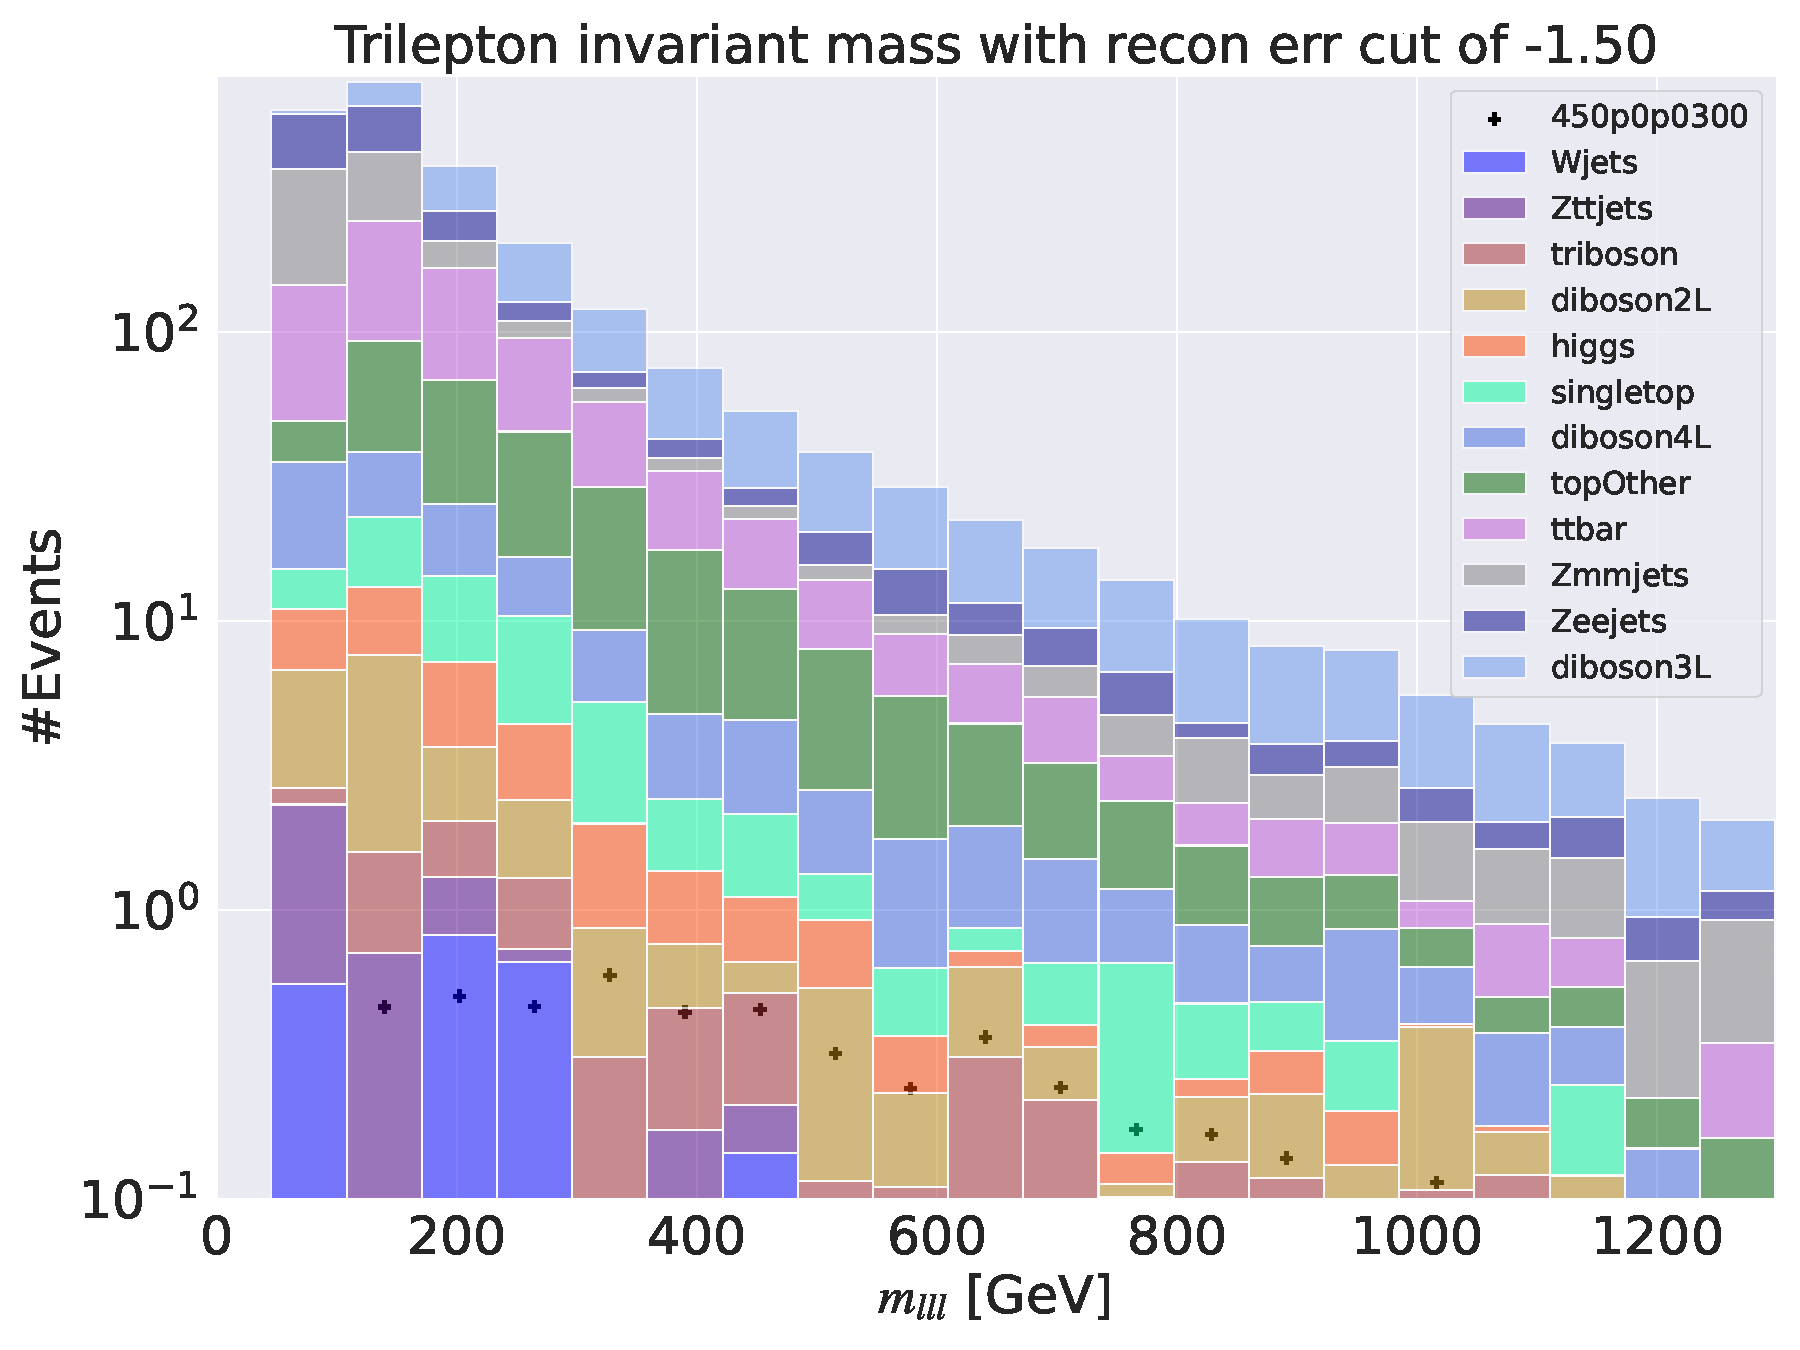
\includegraphics[width=\textwidth]{Figures/AE_testing/big/3lep/b_data_recon_big_rm3_feats_sig_450p0p0300_mlll_recon_errcut_-1.50.pdf}
        \caption{}
        \label{fig:AE_3lep_big_mlll_450}
    \end{subfigure}
    \hfill   
    \begin{subfigure}{.45\textwidth}
        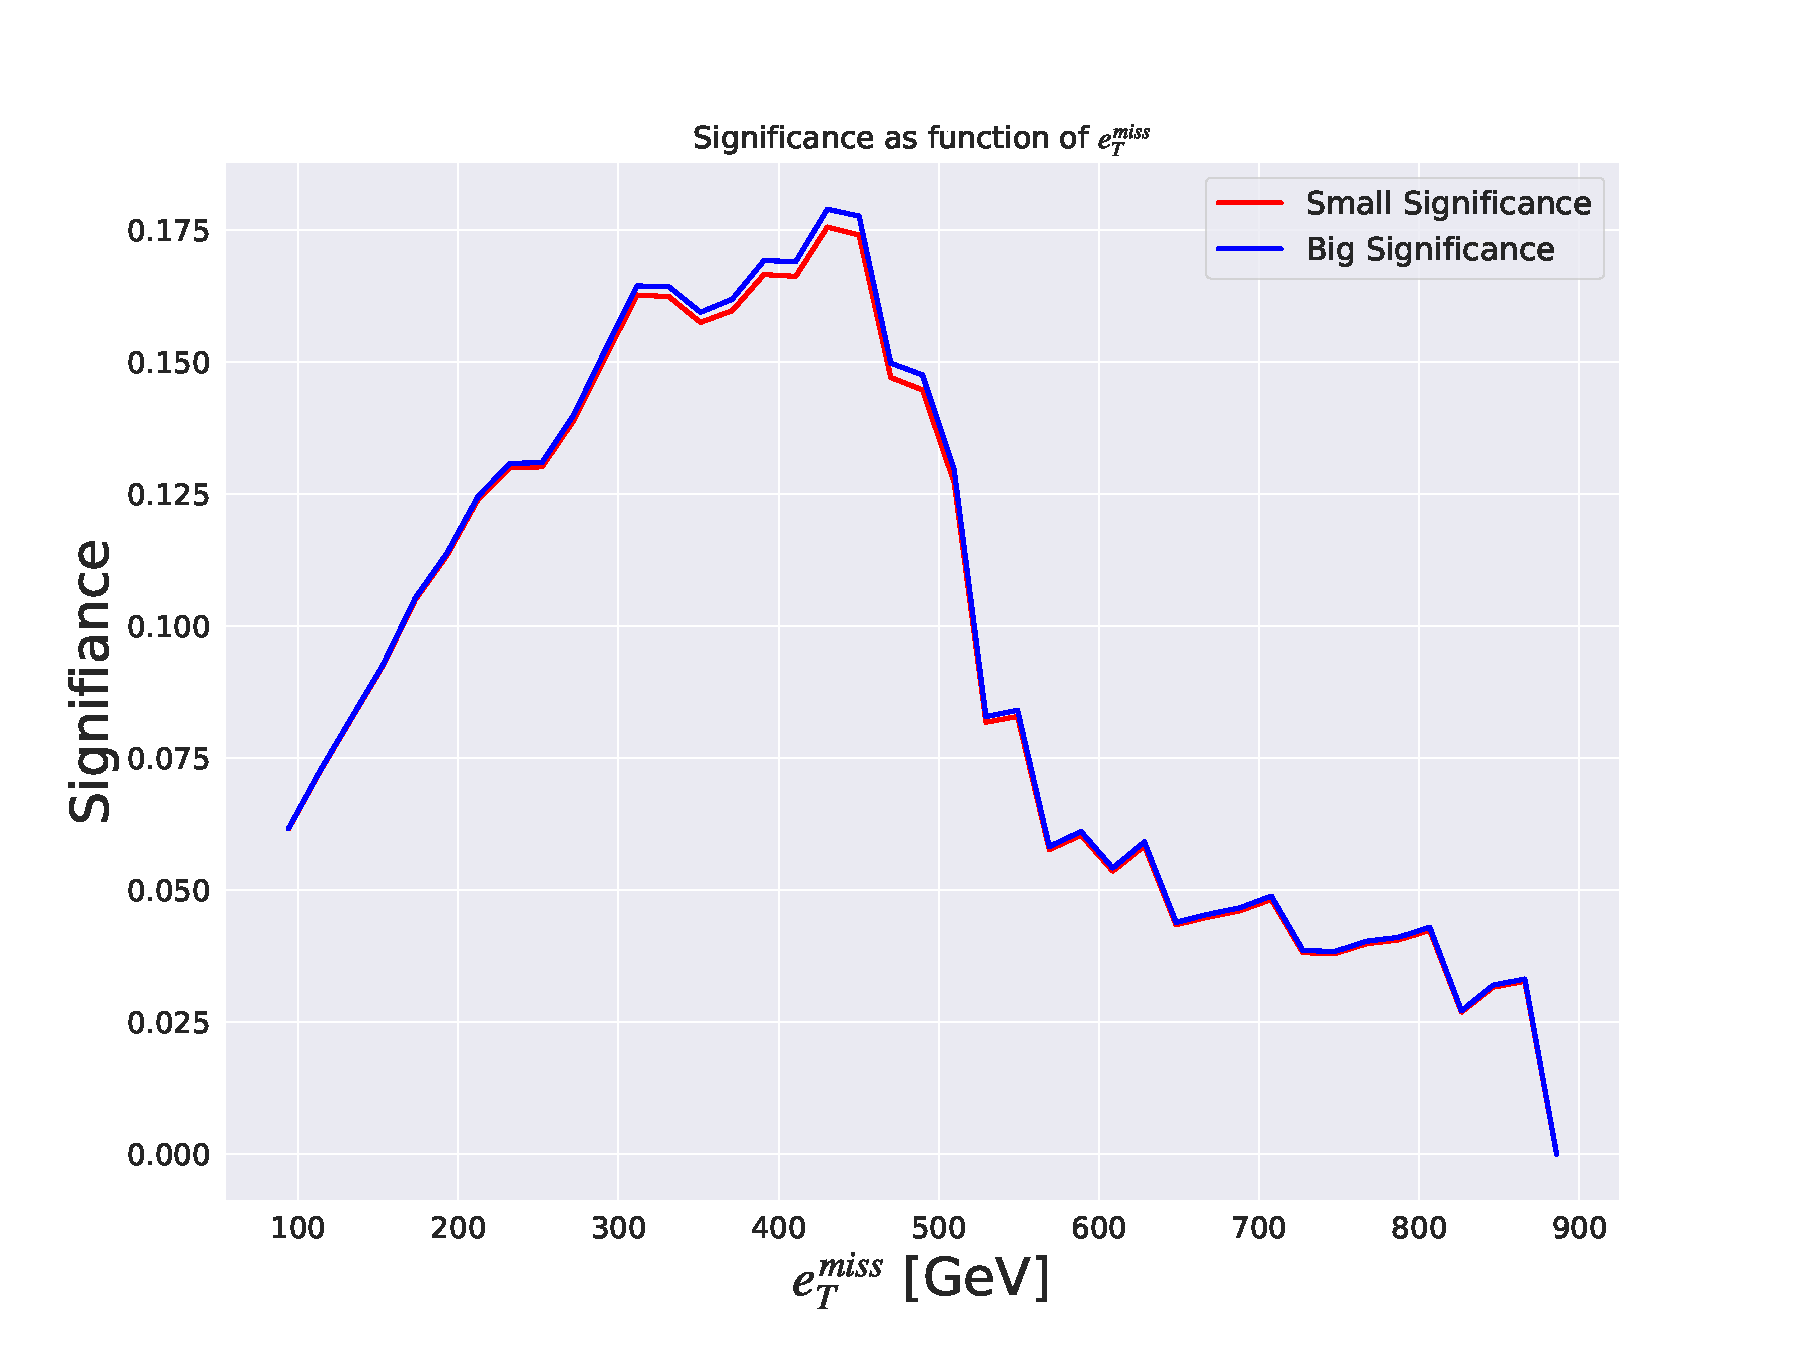
\includegraphics[width=\textwidth]{Figures/AE_testing/big/3lep/significance_etmiss_450p0p0300.pdf}
        \caption{}
        \label{fig:AE_3lep_big_signi_450}
    \end{subfigure}
    \hfill      
    \caption[3lep deep network]{Reconstruction error, $e_T^{miss}$ signal region, $m_{lll}$ signal region and significance as function of 
    $e_T^{miss}$ for the deep regular autoencoder. Here the SUSY $450p300$ model is used.}
    \label{fig:AE_3lep_big_rec_sig_signi_450}
\end{figure}

\begin{figure}[H]
    \centering
    \begin{subfigure}{.45\textwidth}
        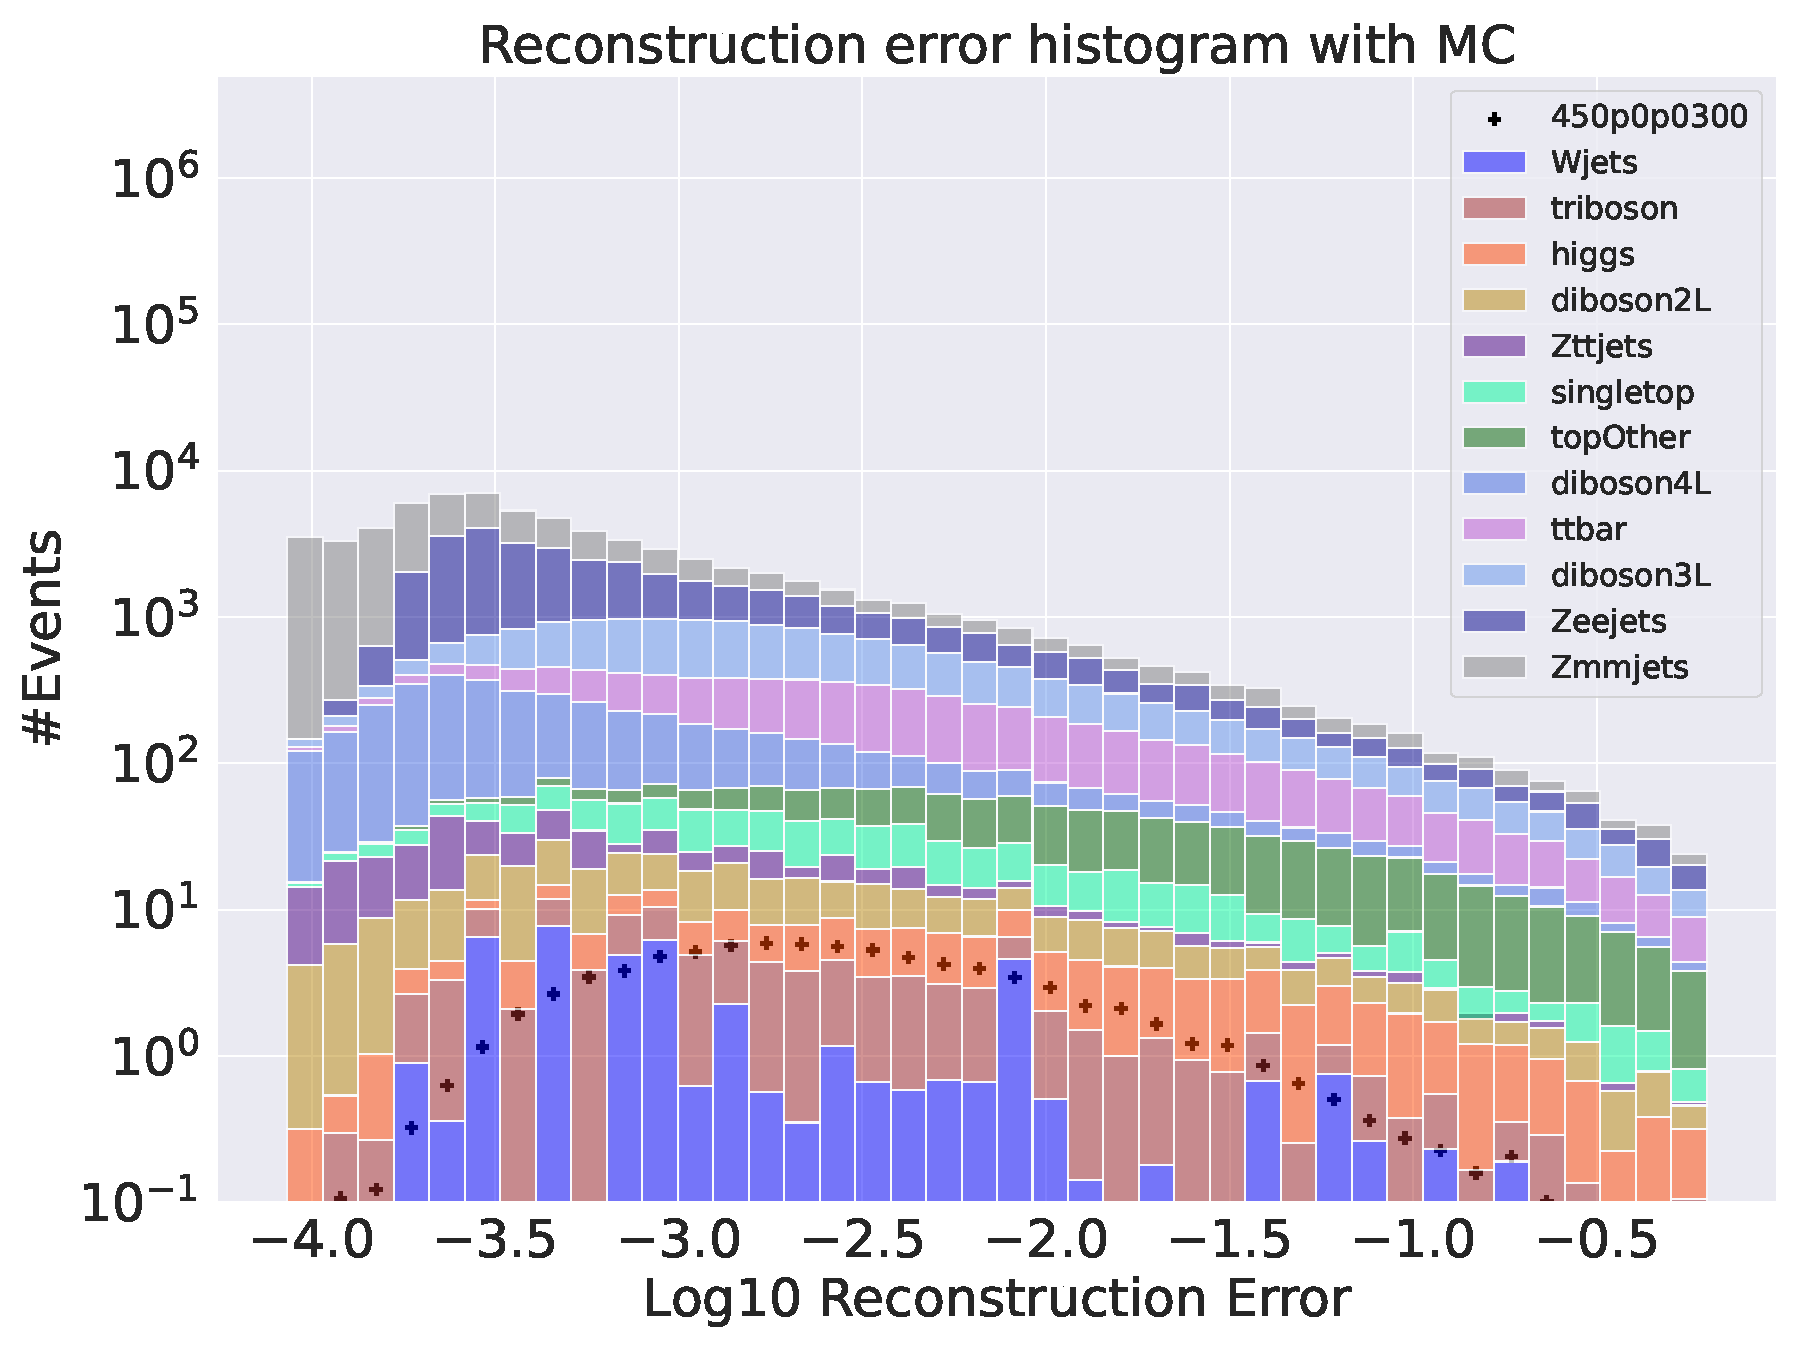
\includegraphics[width=\textwidth]{Figures/AE_testing/small/3lep/b_data_recon_big_rm3_feats_sig_450p0p0300.pdf}
        \caption{ }
        \label{fig:AE_3lep_small_450}
    \end{subfigure}
    \hfill
    \begin{subfigure}{.45\textwidth}
        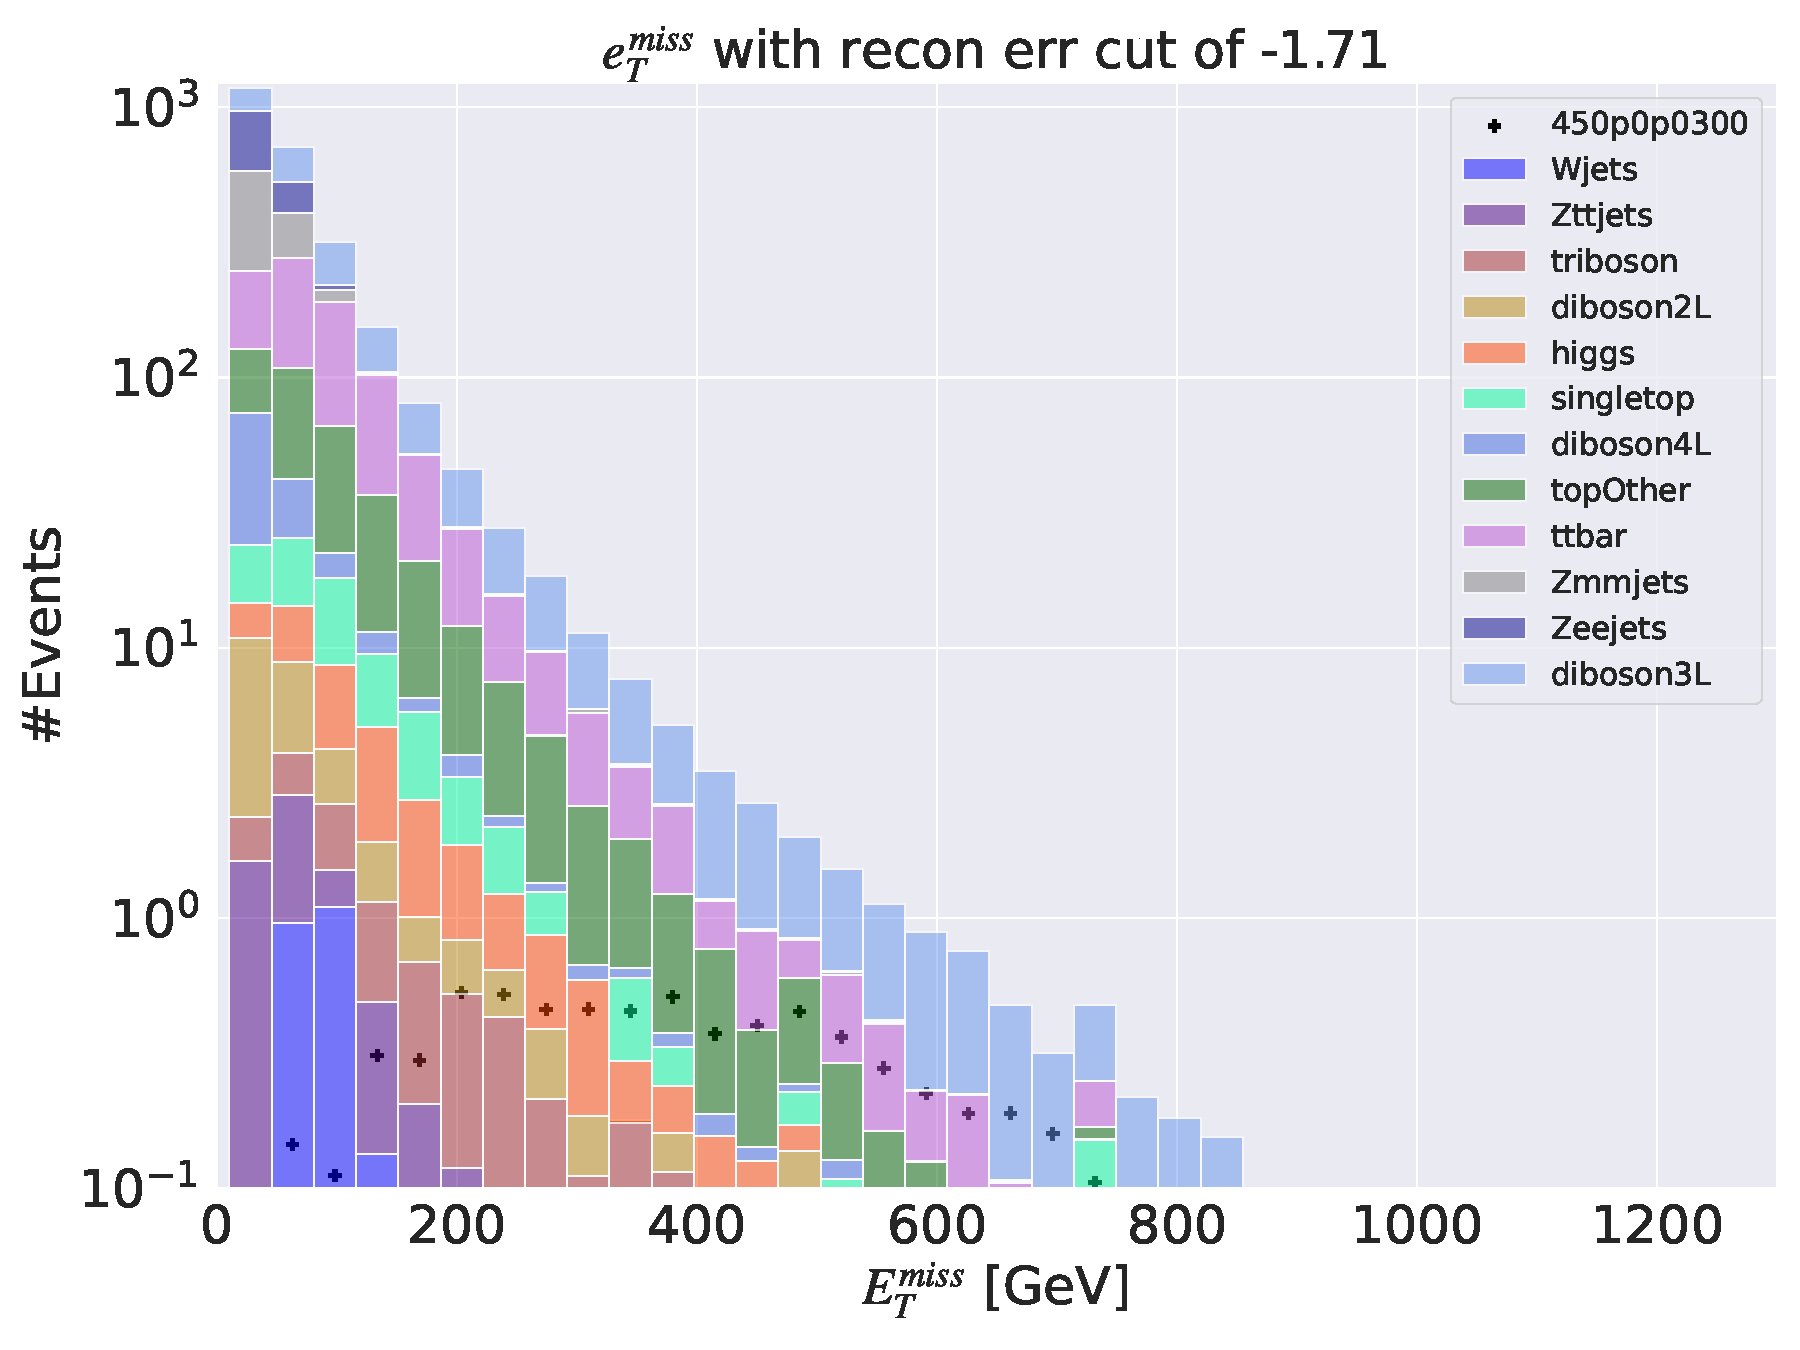
\includegraphics[width=\textwidth]{Figures/AE_testing/small/3lep/b_data_recon_big_rm3_feats_sig_450p0p0300_etmiss_recon_errcut_-1.71.pdf}
        \caption{}
        \label{fig:AE_3lep_small_etmiss_450}
    \end{subfigure}
    \hfill
    \begin{subfigure}{.45\textwidth}
        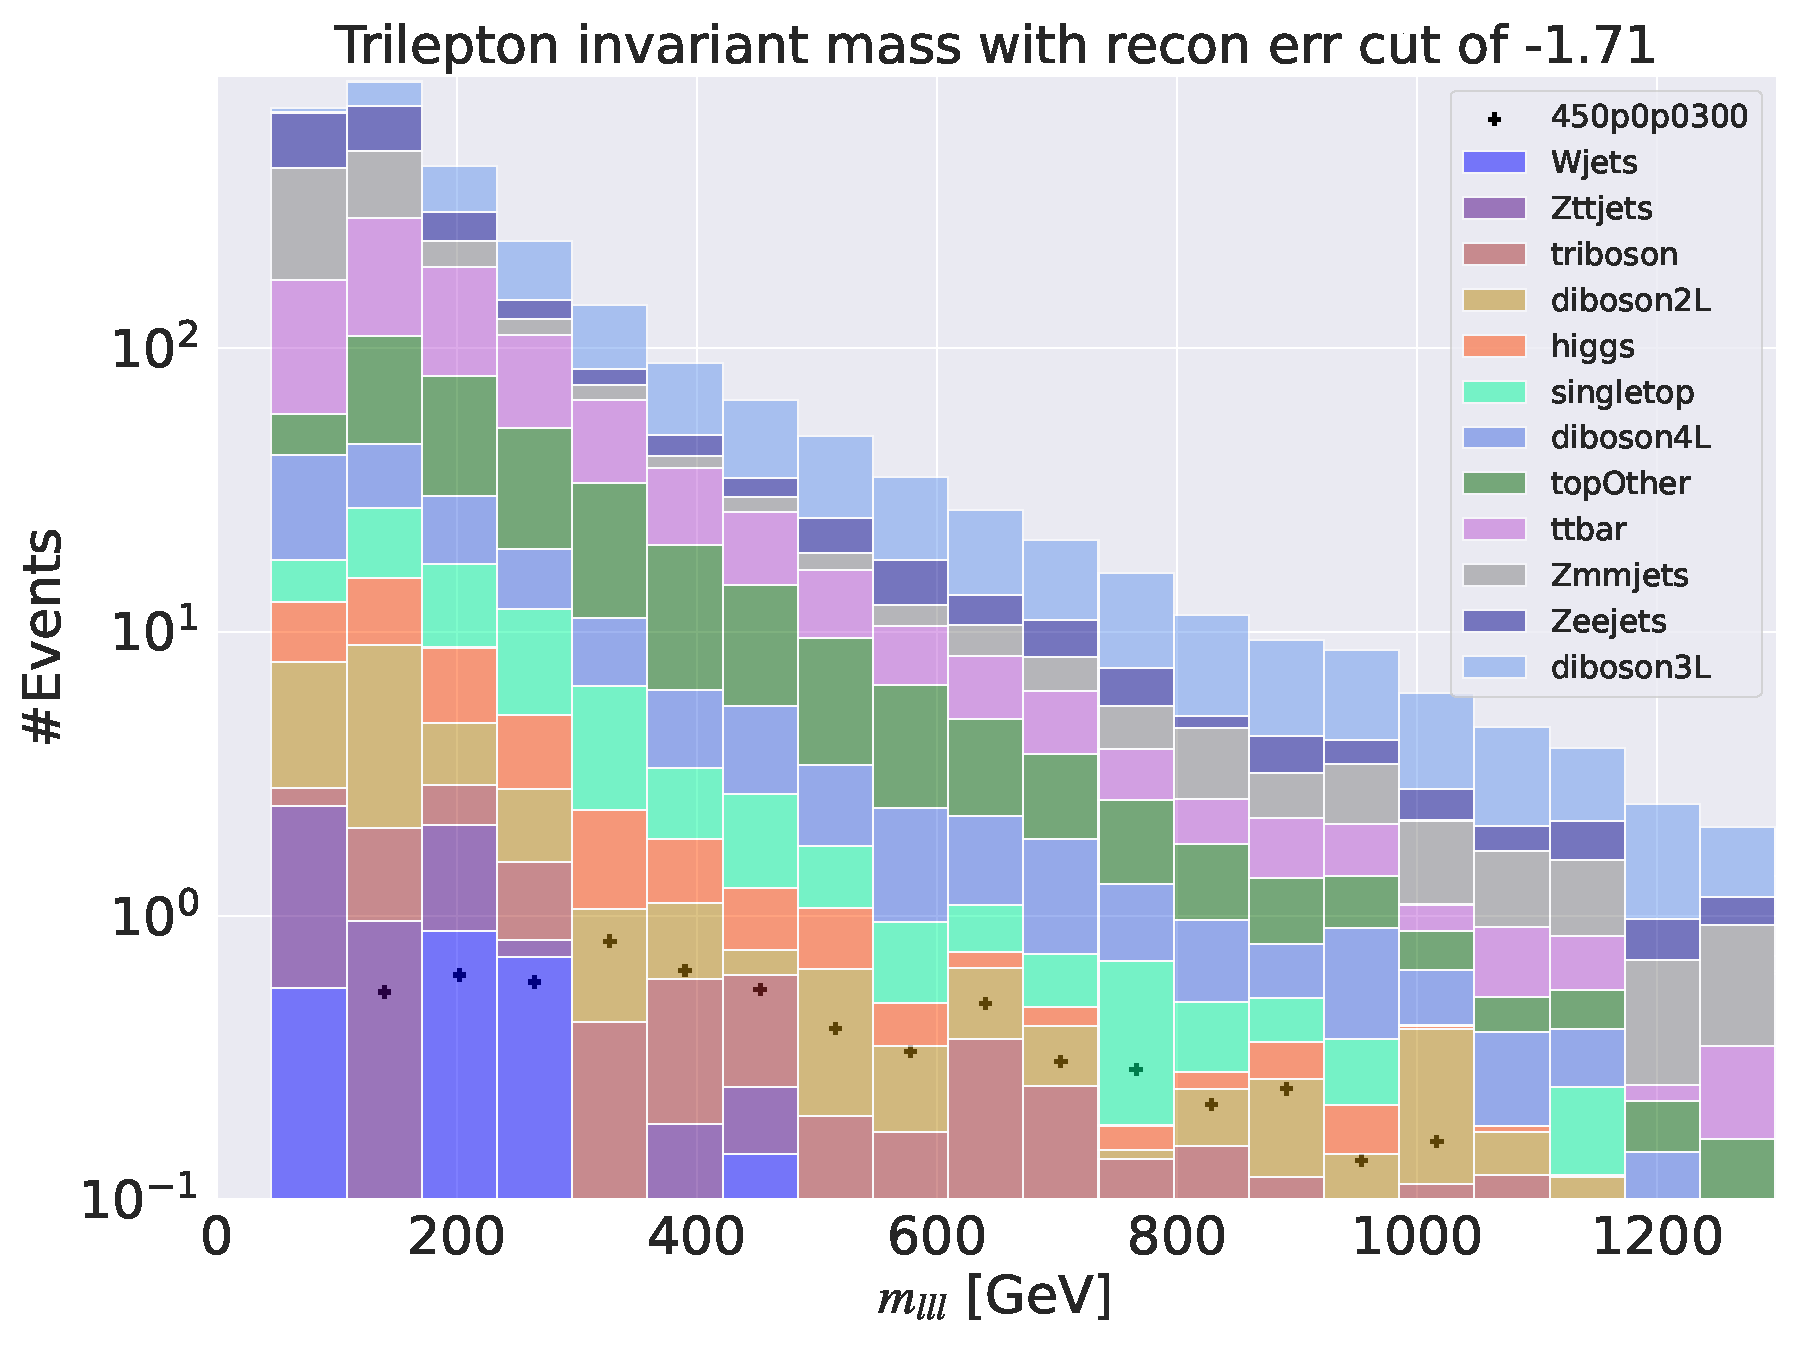
\includegraphics[width=\textwidth]{Figures/AE_testing/small/3lep/b_data_recon_big_rm3_feats_sig_450p0p0300_mlll_recon_errcut_-1.71.pdf}
        \caption{}
        \label{fig:AE_3lep_small_mlll_450}
    \end{subfigure}
    \hfill   
    \begin{subfigure}{.45\textwidth}
        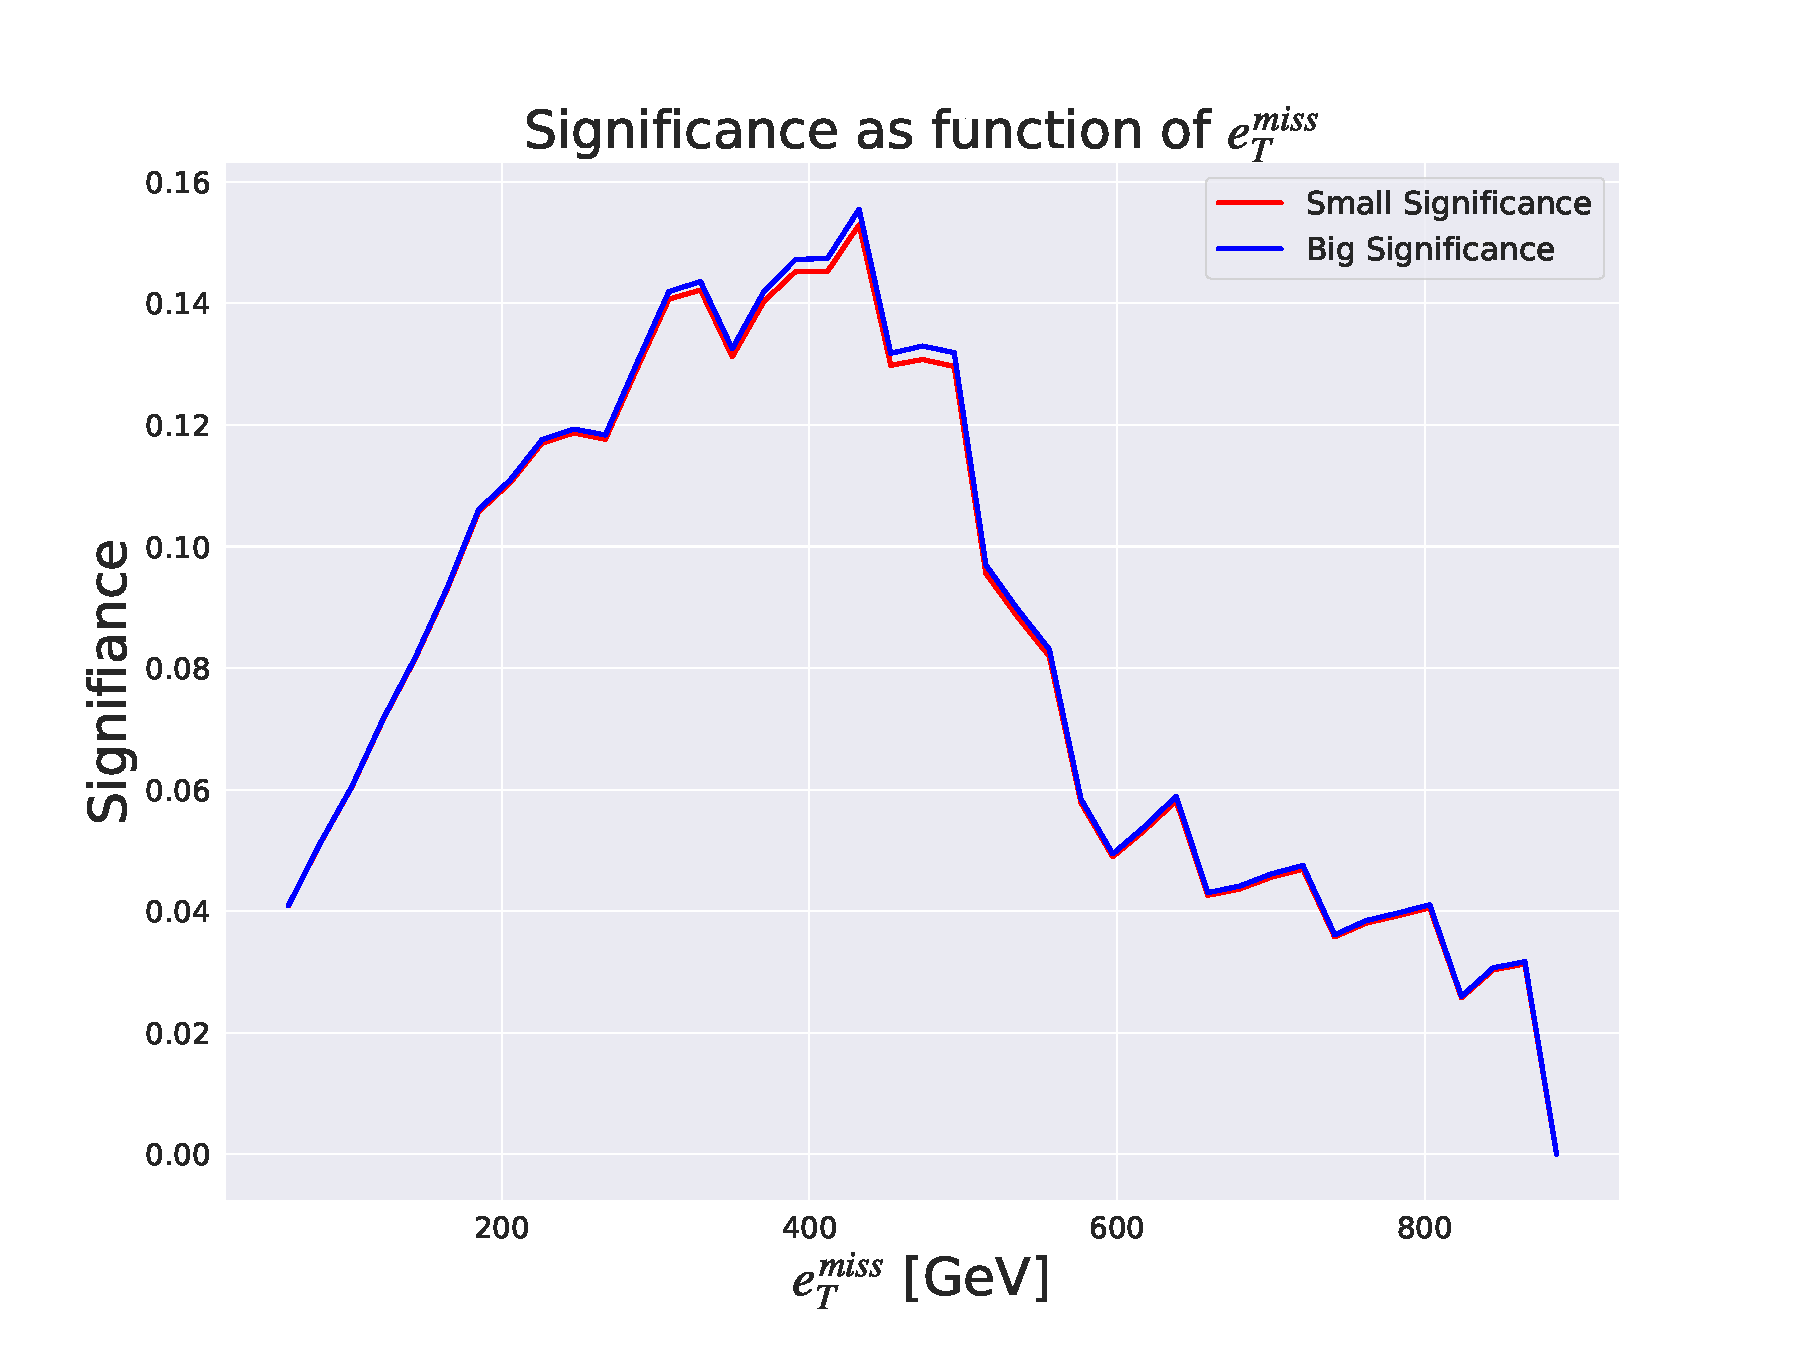
\includegraphics[width=\textwidth]{Figures/AE_testing/small/3lep/significance_etmiss_450p0p0300.pdf}
        \caption{}
        \label{ffig:AE_3lep_small_signi_450}
    \end{subfigure}
    \hfill      
    \caption[3lep deep network]{Reconstruction error, $e_T^{miss}$ signal region, $m_{lll}$ signal region and significance as function of 
    $e_T^{miss}$ for the deep regular autoencoder. Here the SUSY $450p300$ model is used.}
    \label{fig:AE_3lep_small_rec_sig_signi_450}
\end{figure}








\begin{figure}[H]
    \centering
    \begin{subfigure}{.45\textwidth}
        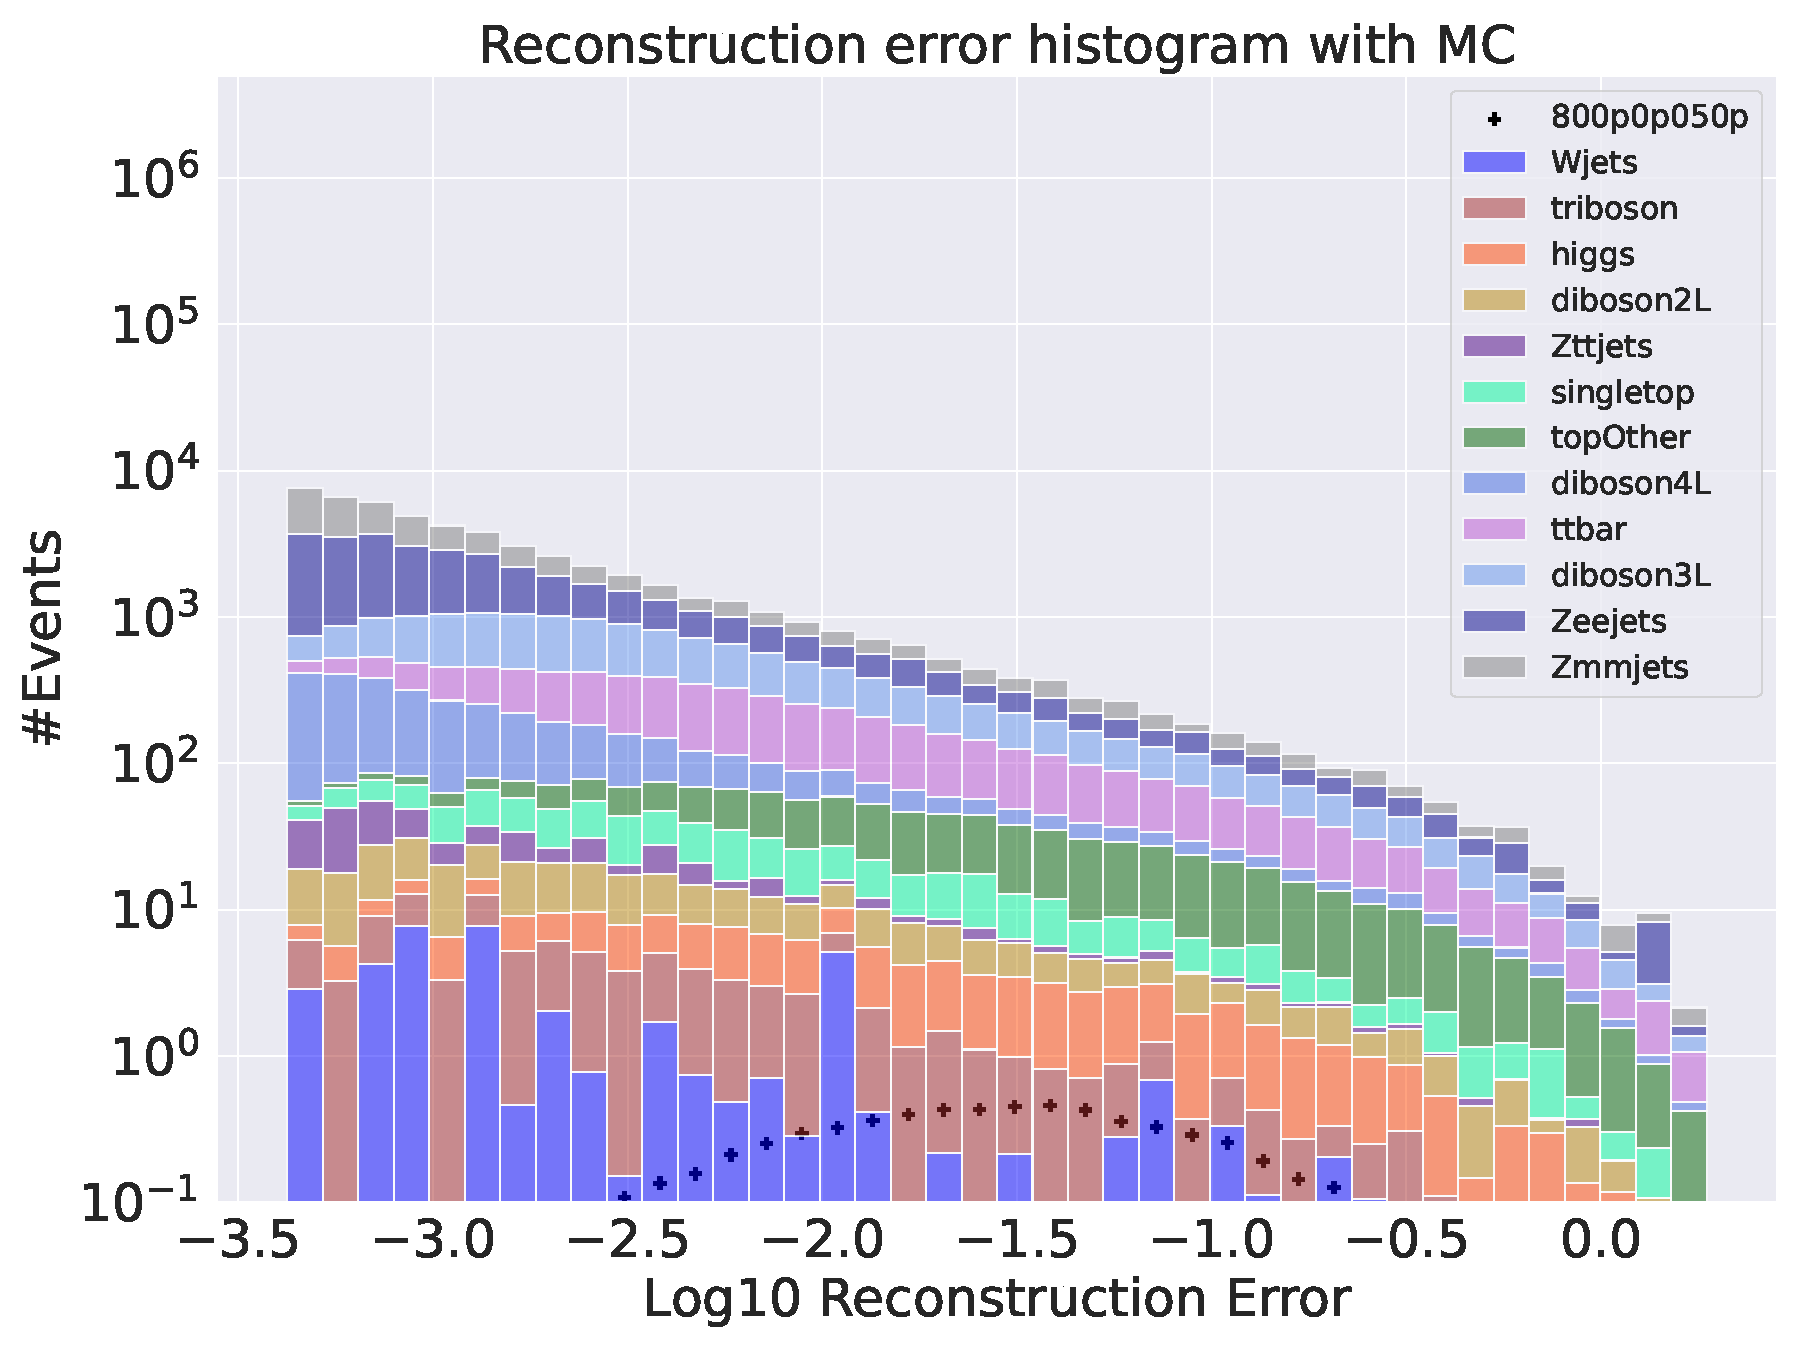
\includegraphics[width=\textwidth]{Figures/AE_testing/big/3lep/b_data_recon_big_rm3_feats_sig_800p0p050p.pdf}
        \caption{ }
        \label{fig:AE_3lep_big_800}
    \end{subfigure}
    \hfill
    \begin{subfigure}{.45\textwidth}
        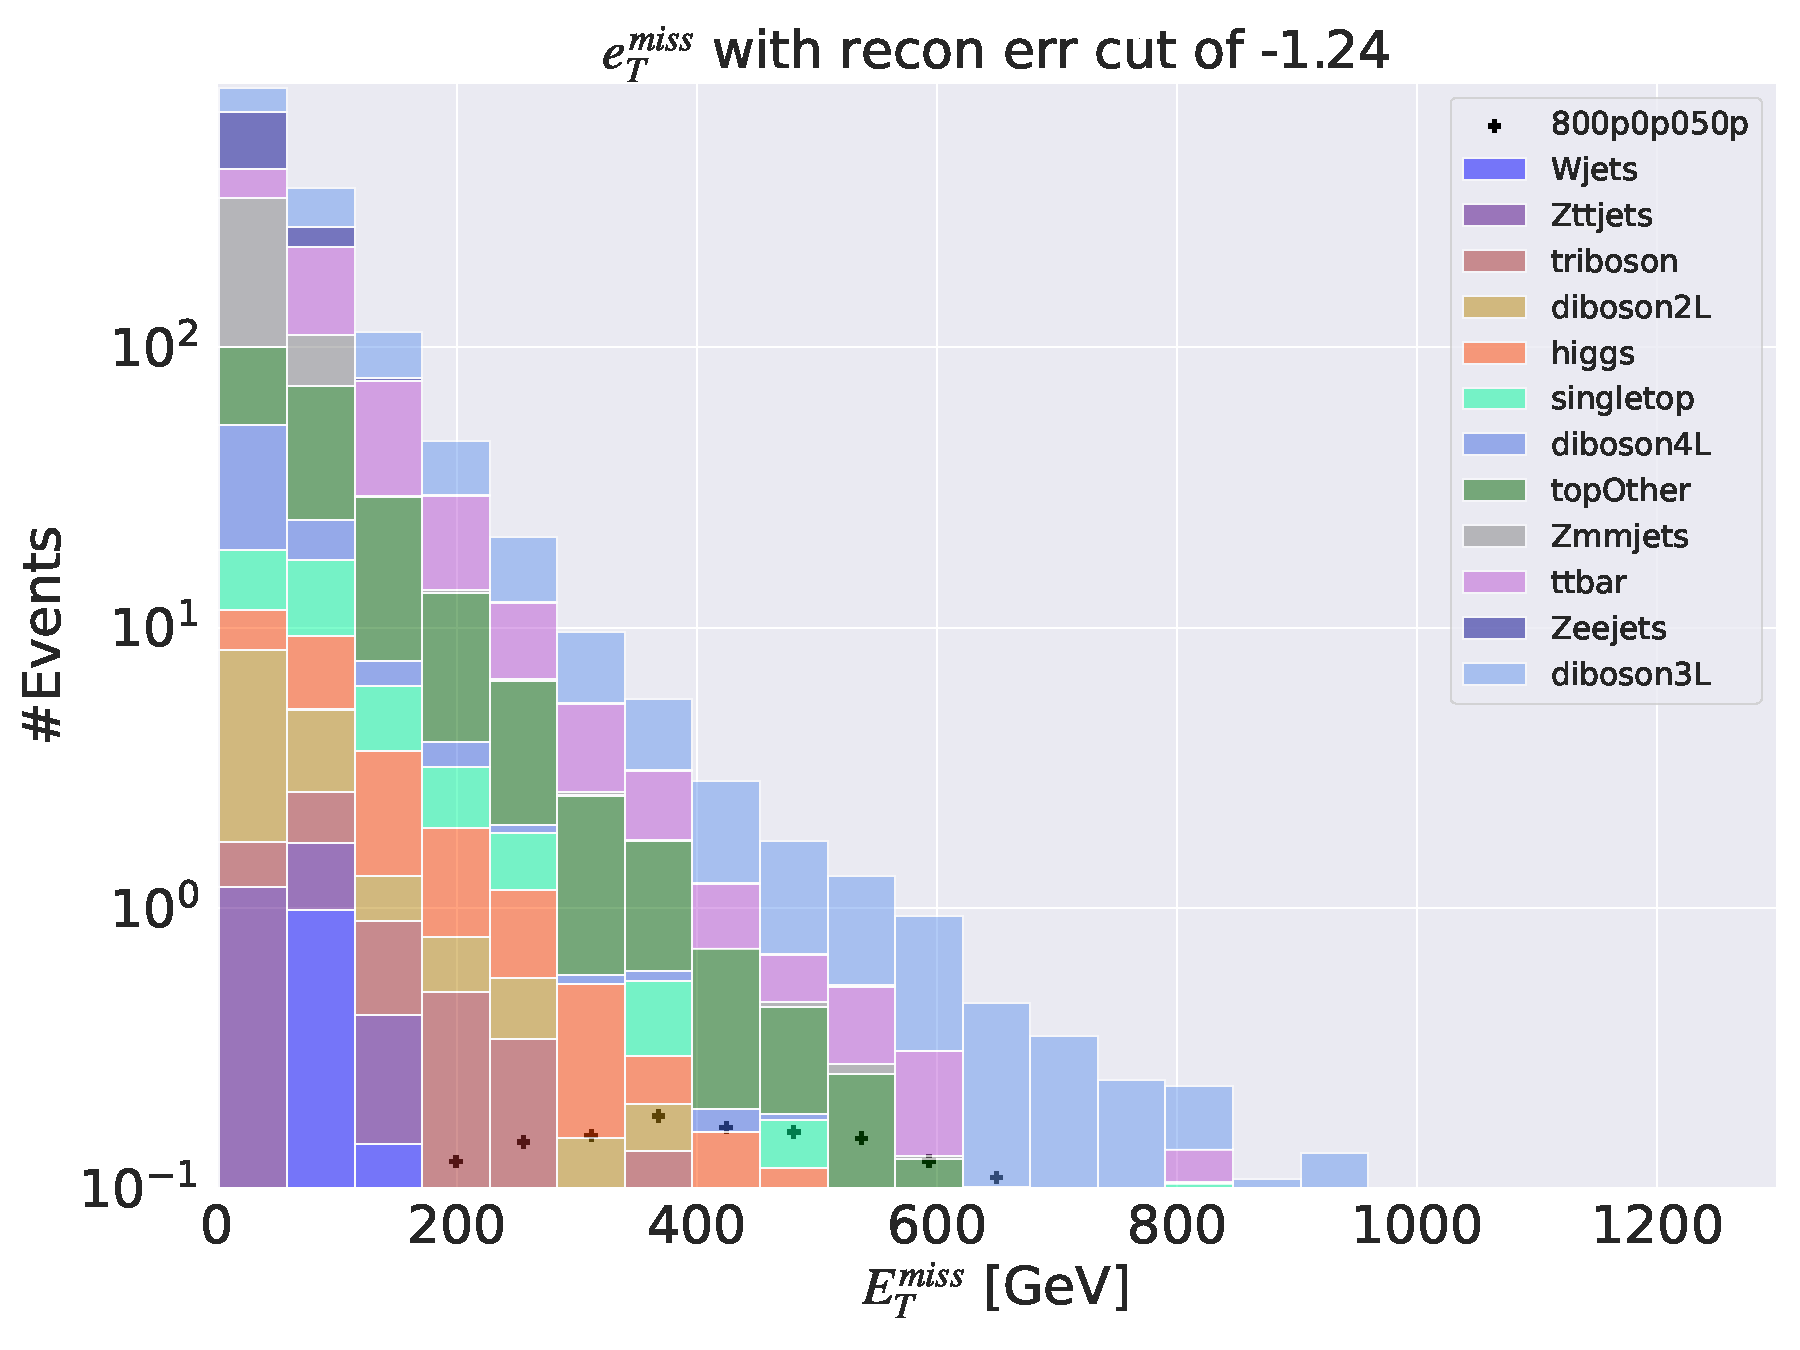
\includegraphics[width=\textwidth]{Figures/AE_testing/big/3lep/b_data_recon_big_rm3_feats_sig_800p0p050p_etmiss_recon_errcut_-1.24.pdf}
        \caption{}
        \label{fig:AE_3lep_big_etmiss_800}
    \end{subfigure}
    \hfill
    \begin{subfigure}{.45\textwidth}
        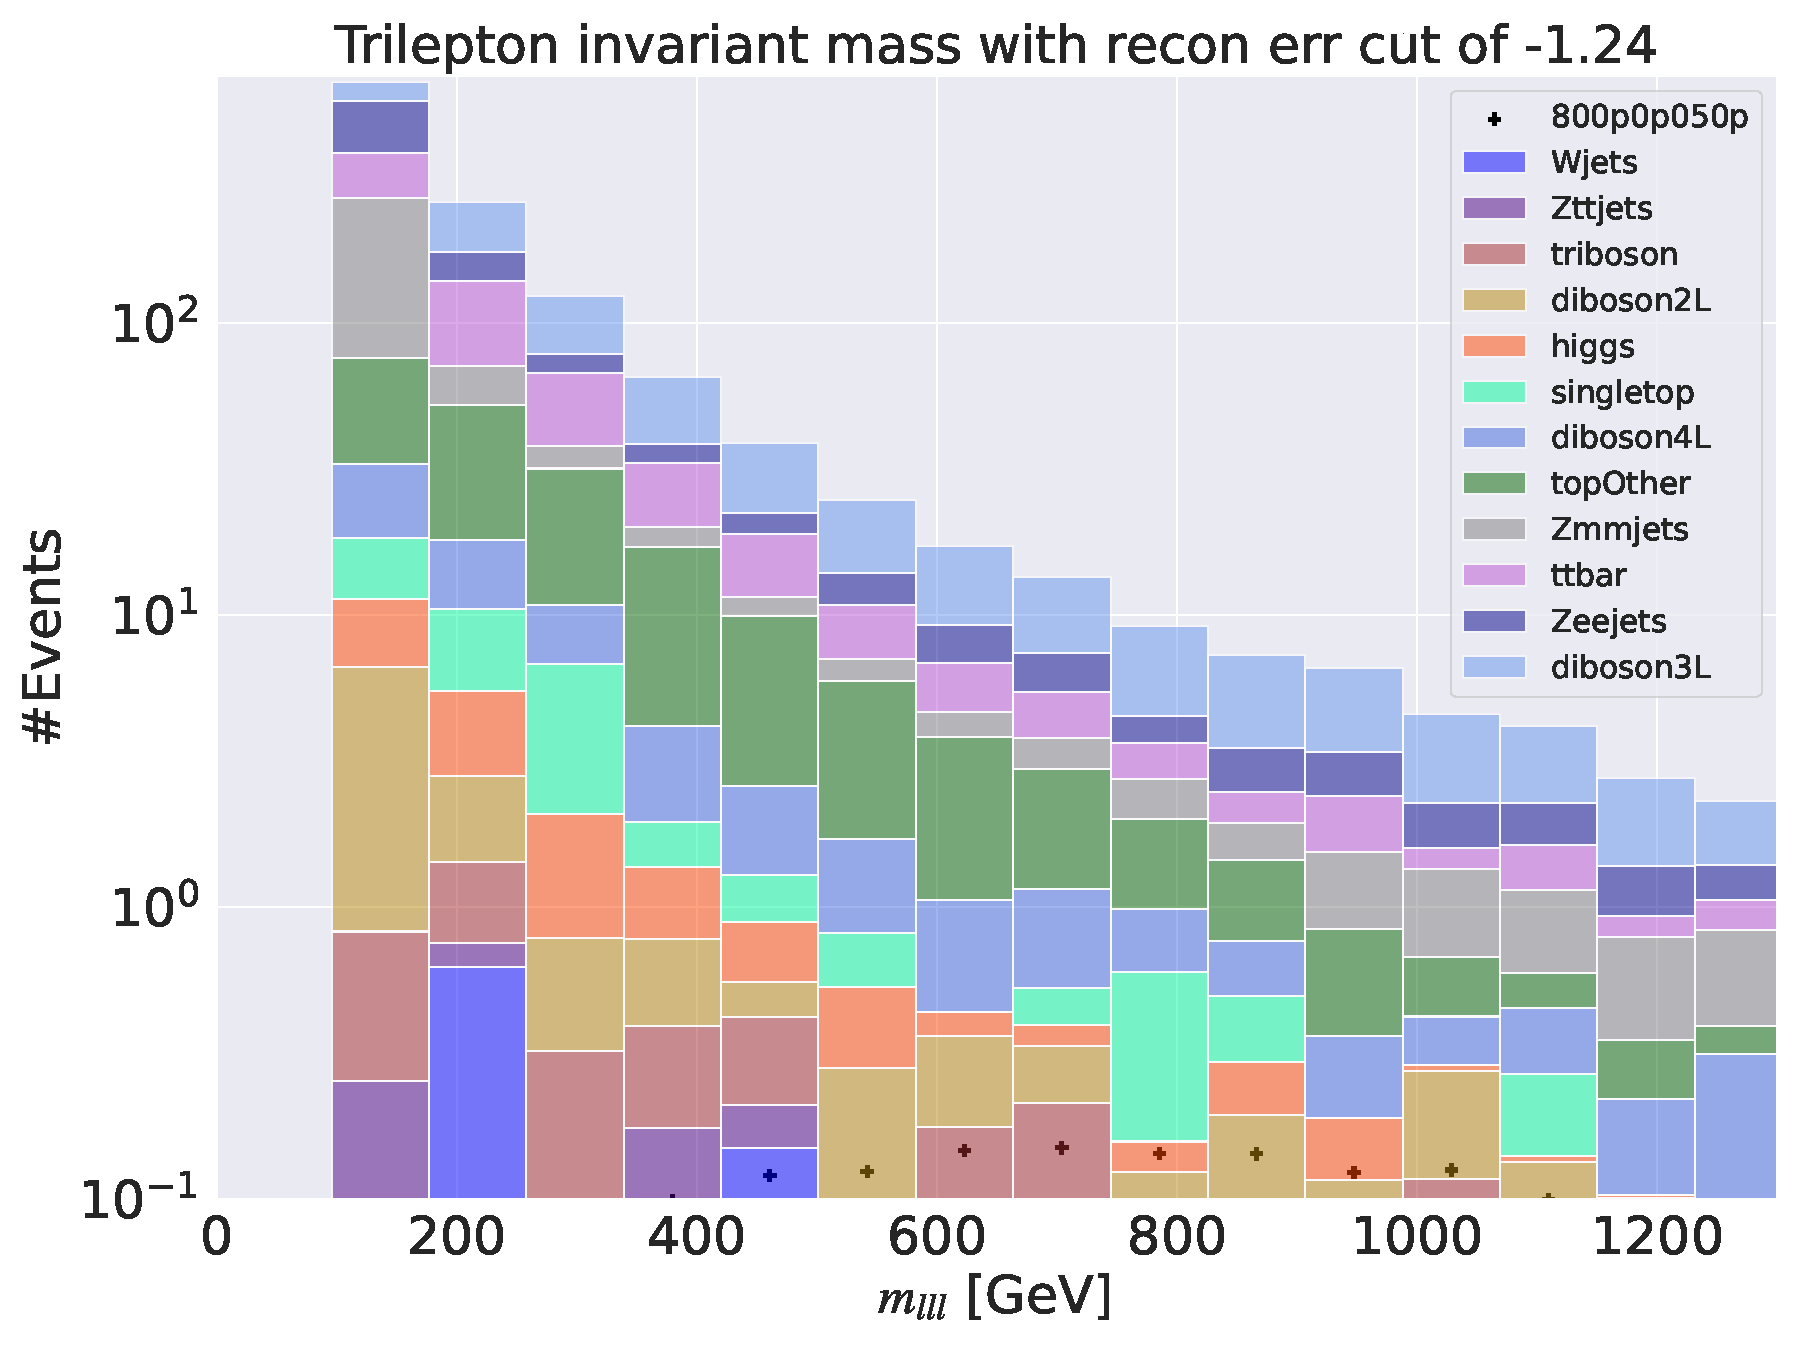
\includegraphics[width=\textwidth]{Figures/AE_testing/big/3lep/b_data_recon_big_rm3_feats_sig_800p0p050p_mlll_recon_errcut_-1.24.pdf}
        \caption{}
        \label{fig:AE_3lep_big_mlll_800}
    \end{subfigure}
    \hfill   
    \begin{subfigure}{.45\textwidth}
        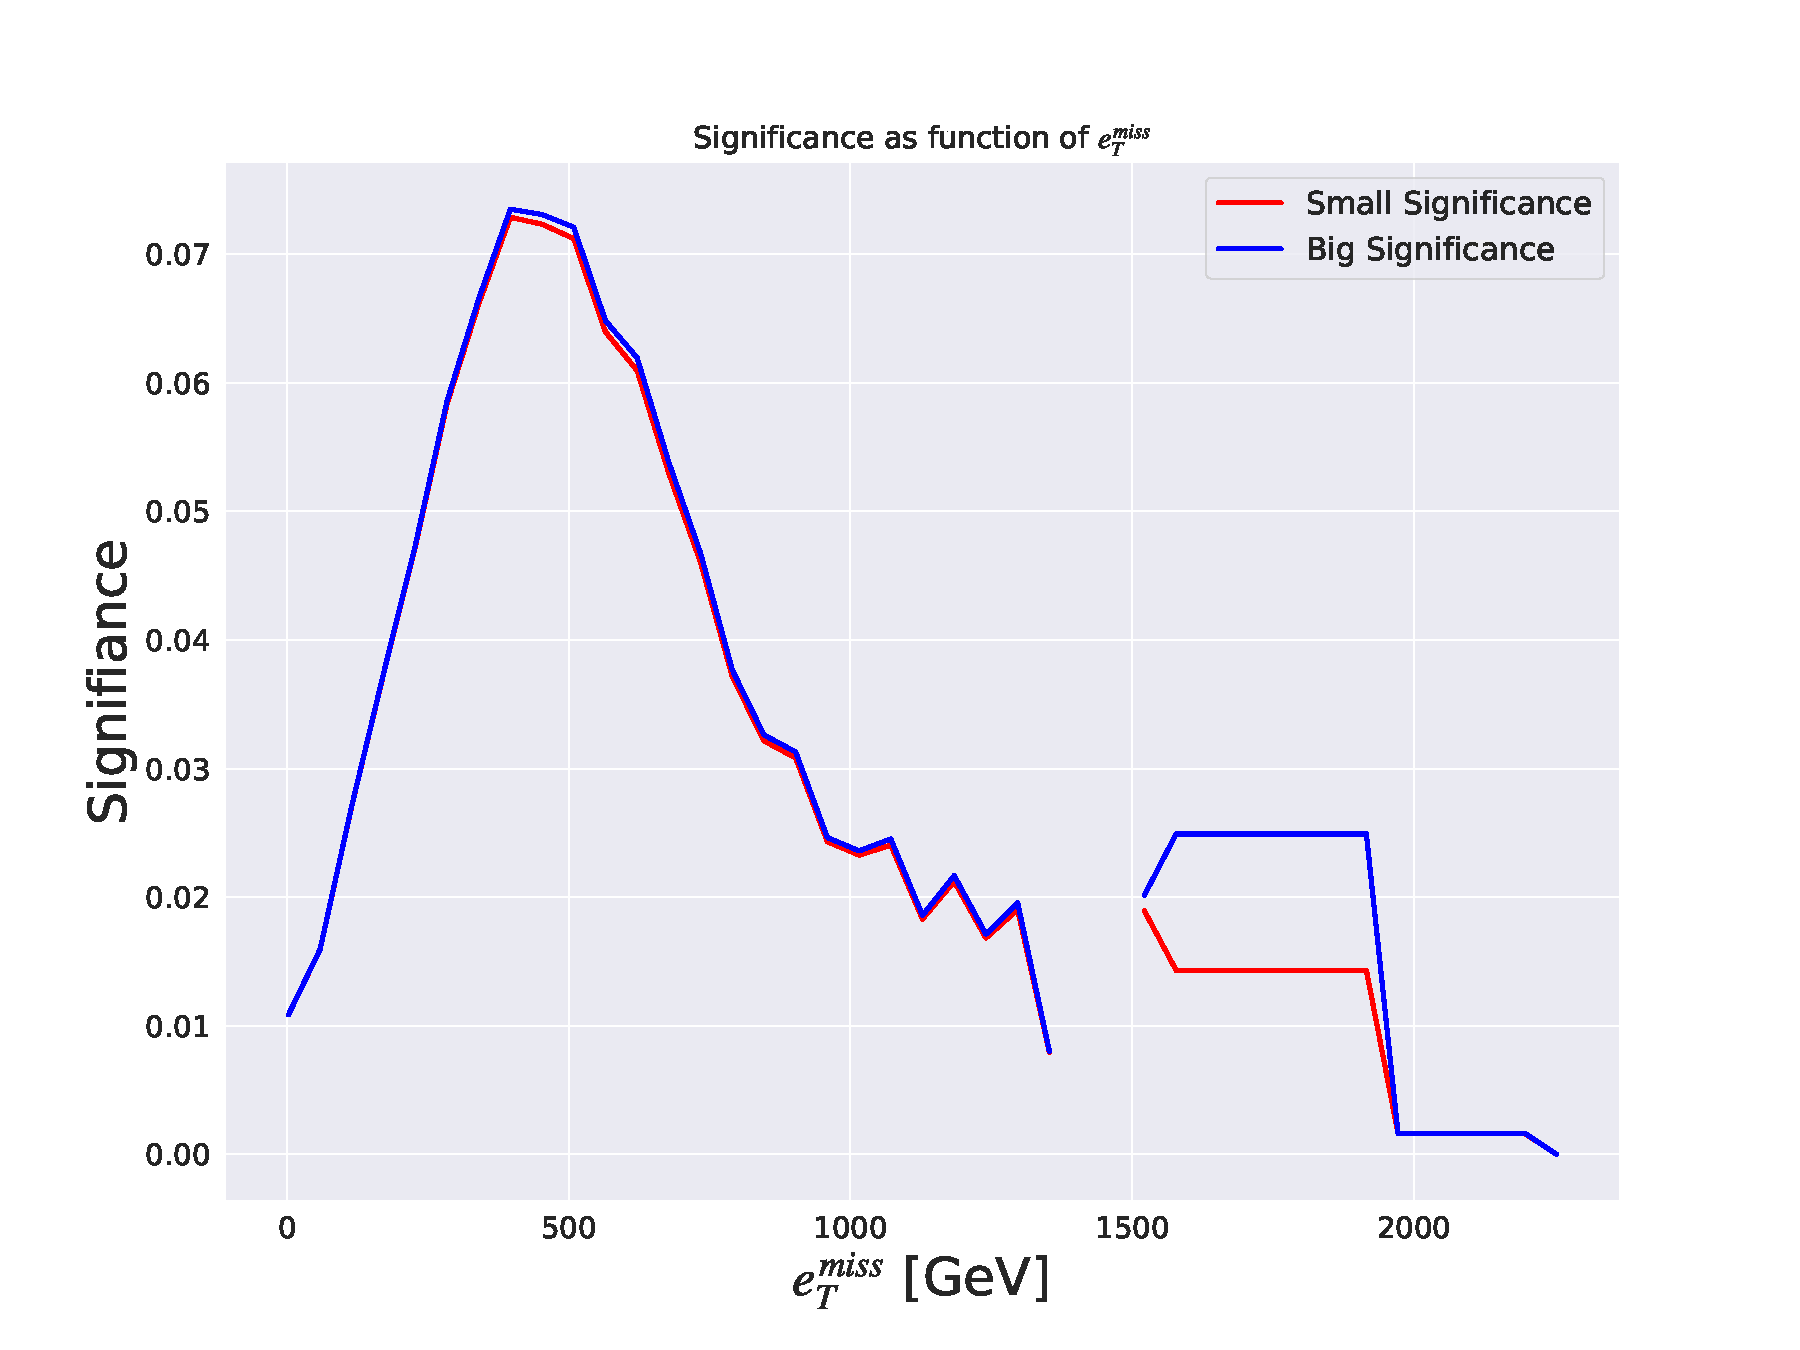
\includegraphics[width=\textwidth]{Figures/AE_testing/big/3lep/significance_etmiss_800p0p050p.pdf}
        \caption{}
        \label{fig:AE_3lep_big_signi_800}
    \end{subfigure}
    \hfill      
    \caption[3lep deep network]{Reconstruction error, $e_T^{miss}$ signal region, $m_{lll}$ signal region and significance as function of 
    $e_T^{miss}$ for the deep regular autoencoder. Here the SUSY $450p300$ model is used.}
    \label{fig:AE_3lep_big_rec_sig_signi_800}
\end{figure}

\begin{figure}[H]
    \centering
    \begin{subfigure}{.45\textwidth}
        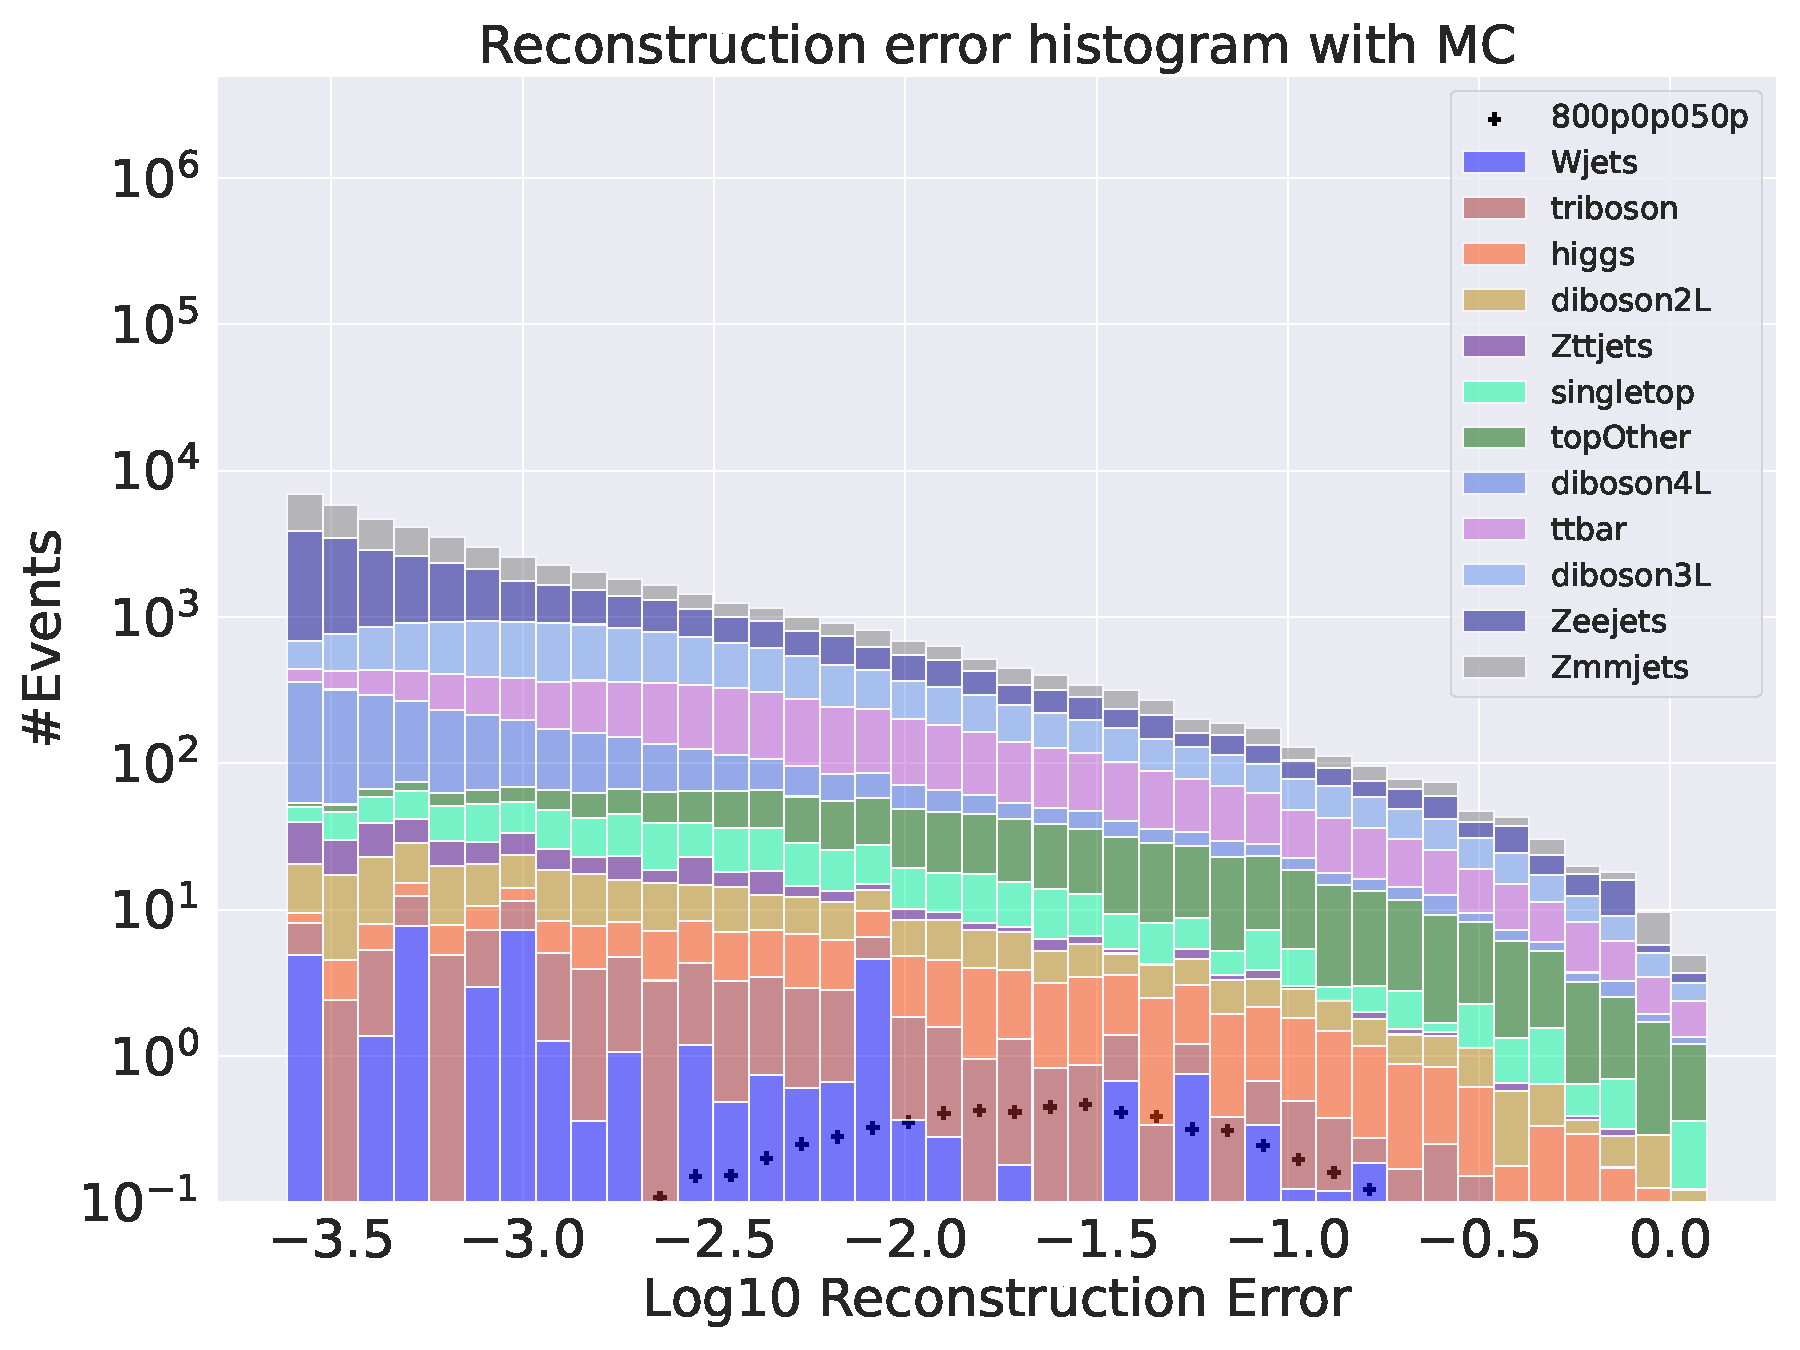
\includegraphics[width=\textwidth]{Figures/AE_testing/small/3lep/b_data_recon_big_rm3_feats_sig_800p0p050p.pdf}
        \caption{ }
        \label{fig:AE_3lep_small_800}
    \end{subfigure}
    \hfill
    \begin{subfigure}{.45\textwidth}
        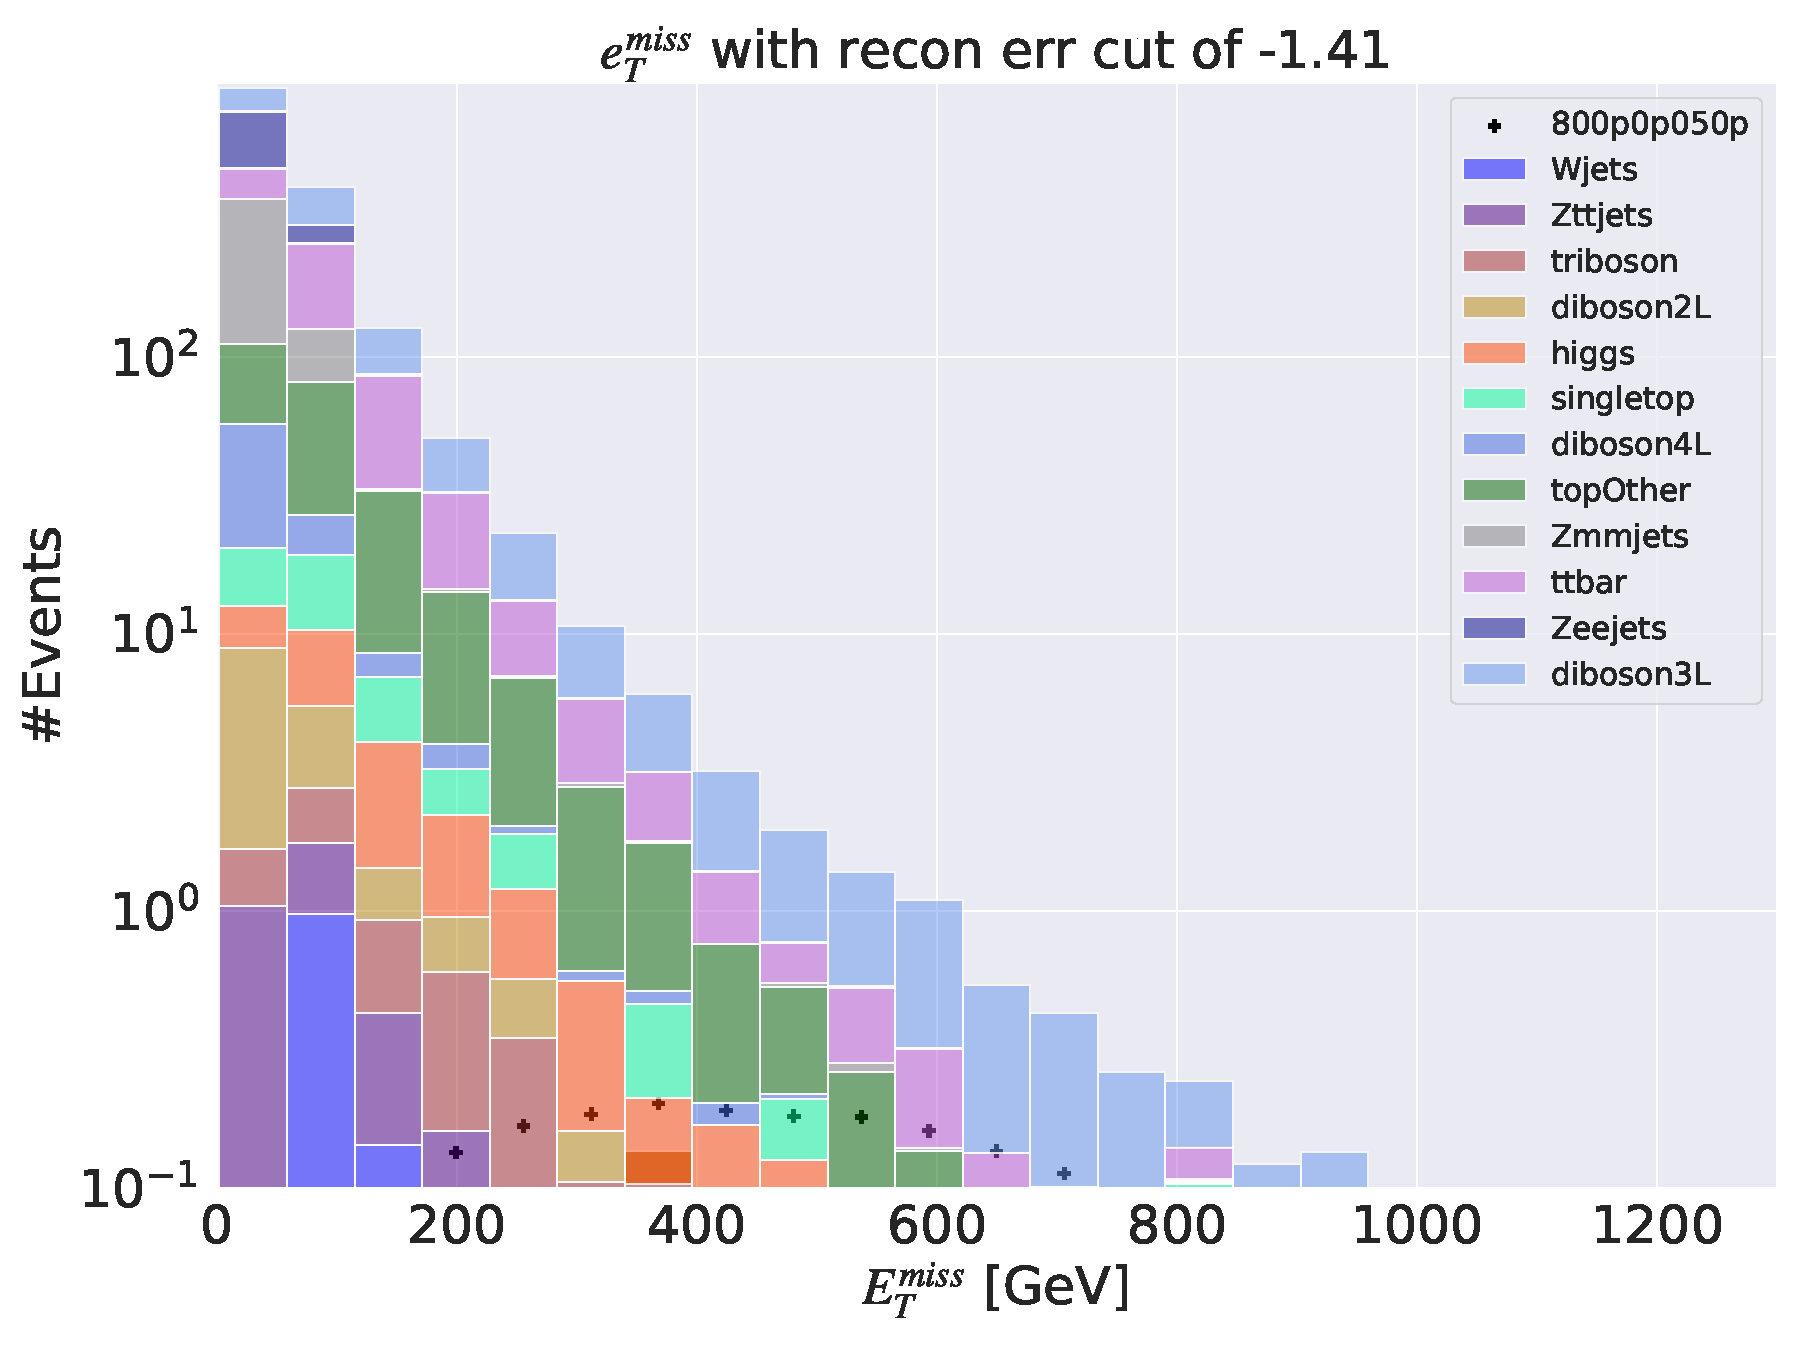
\includegraphics[width=\textwidth]{Figures/AE_testing/small/3lep/b_data_recon_big_rm3_feats_sig_800p0p050p_etmiss_recon_errcut_-1.41.pdf}
        \caption{}
        \label{fig:AE_3lep_small_etmiss_800}
    \end{subfigure}
    \hfill
    \begin{subfigure}{.45\textwidth}
        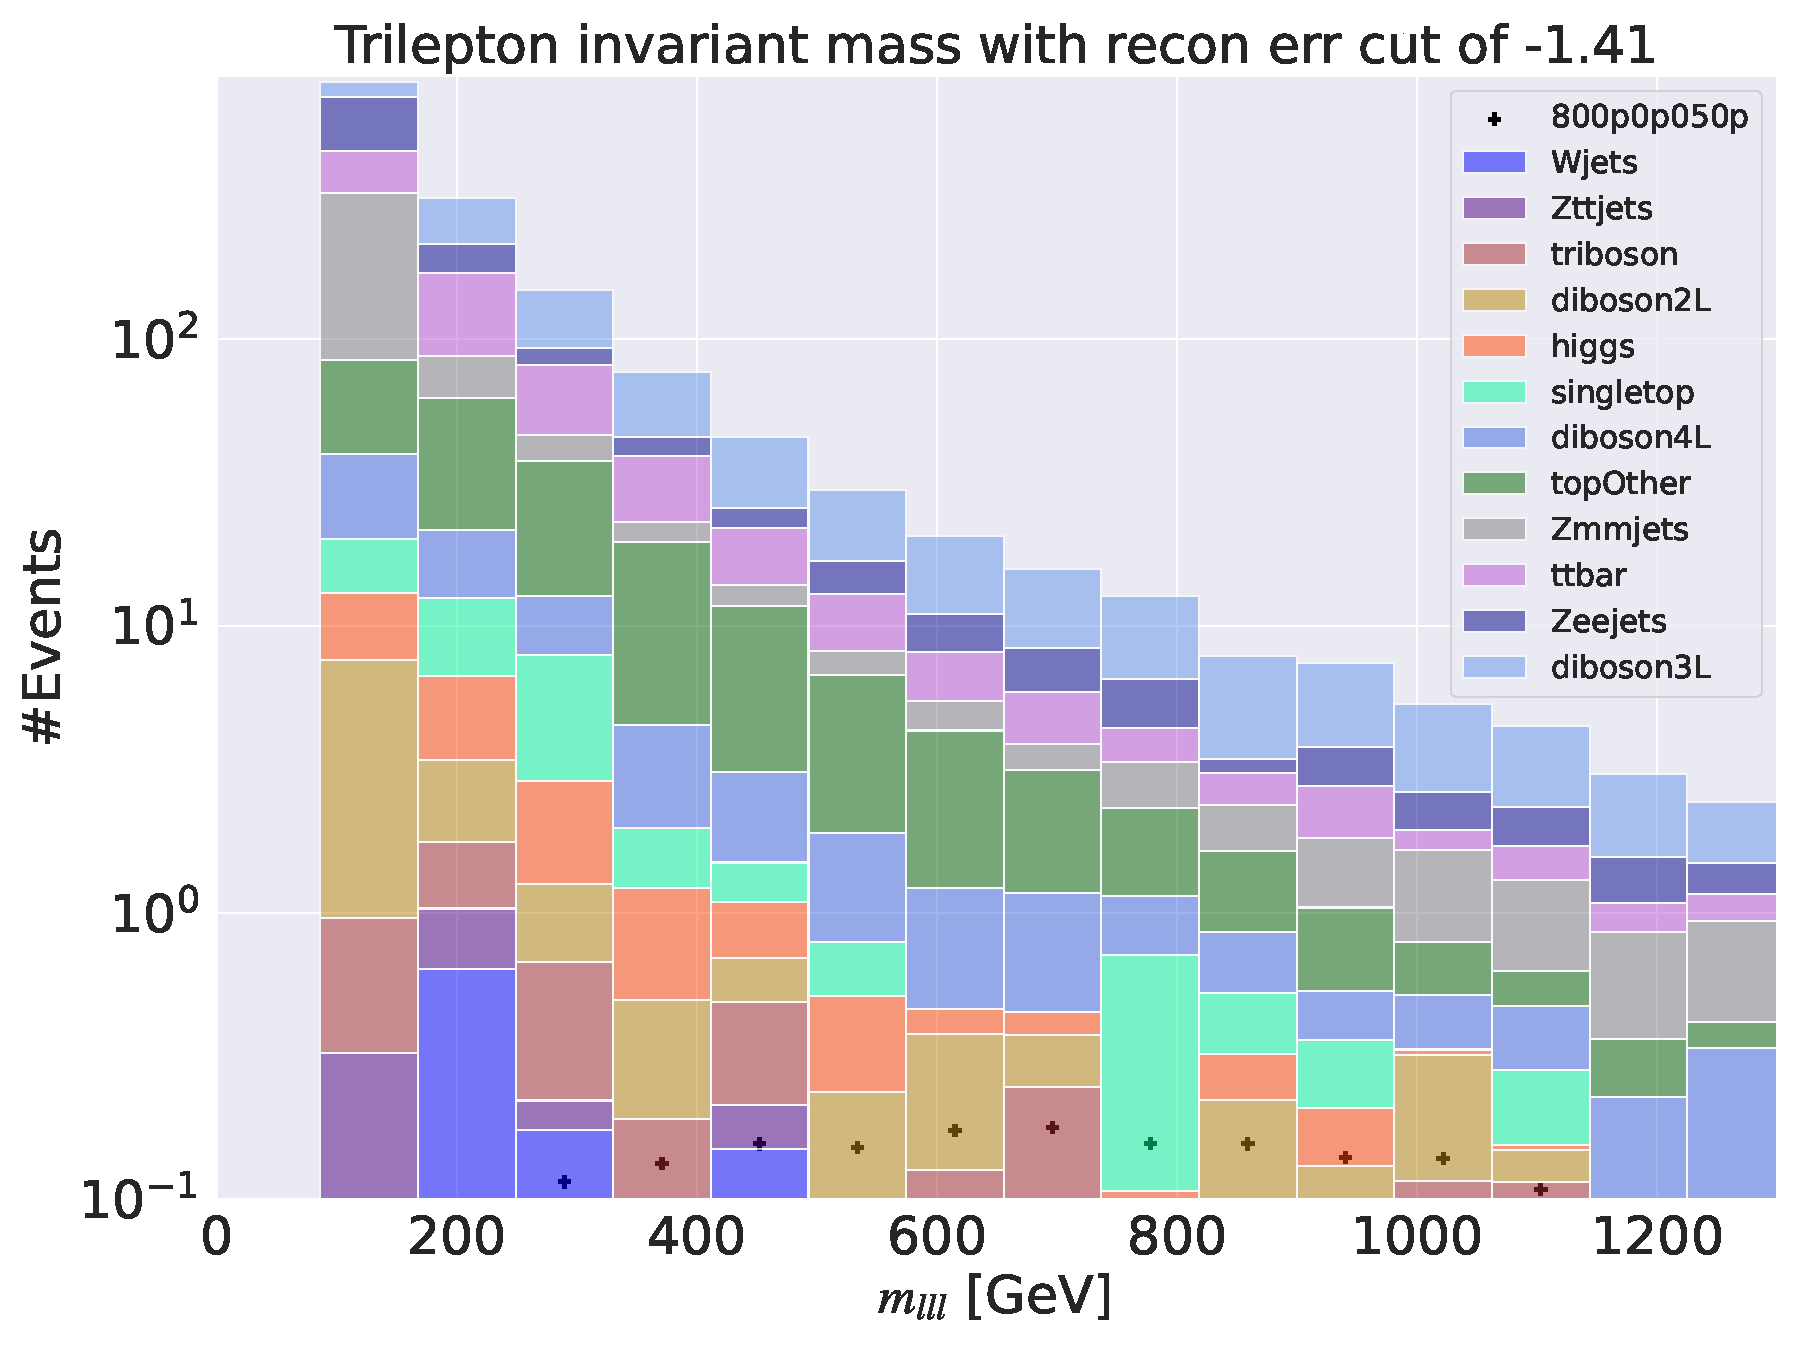
\includegraphics[width=\textwidth]{Figures/AE_testing/small/3lep/b_data_recon_big_rm3_feats_sig_800p0p050p_mlll_recon_errcut_-1.41.pdf}
        \caption{}
        \label{fig:AE_3lep_small_mlll_800}
    \end{subfigure}
    \hfill   
    \begin{subfigure}{.45\textwidth}
        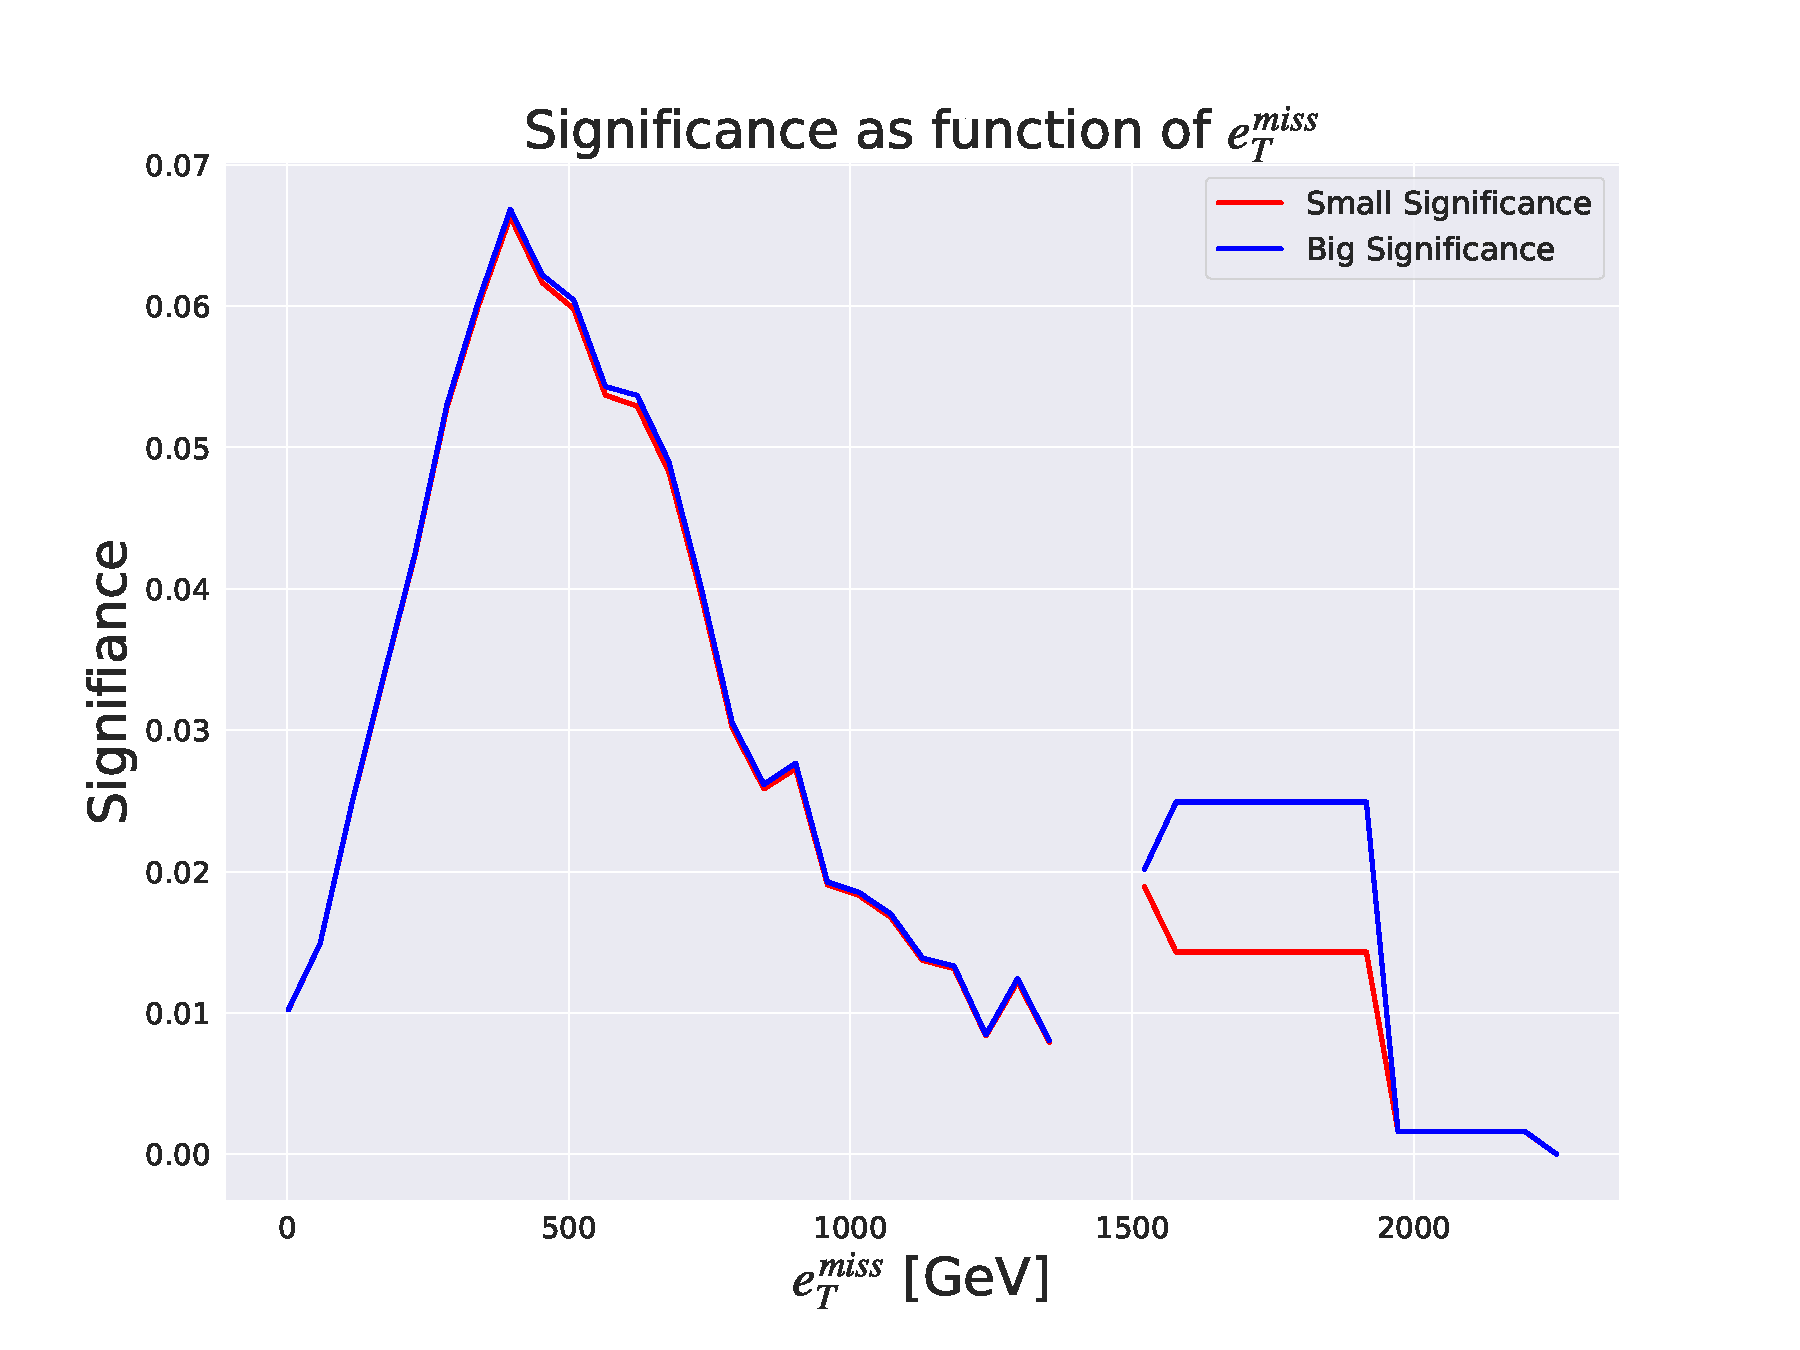
\includegraphics[width=\textwidth]{Figures/AE_testing/small/3lep/significance_etmiss_800p0p050p.pdf}
        \caption{}
        \label{ffig:AE_3lep_small_signi_800}
    \end{subfigure}
    \hfill      
    \caption[3lep deep network]{Reconstruction error, $e_T^{miss}$ signal region, $m_{lll}$ signal region and significance as function of 
    $e_T^{miss}$ for the deep regular autoencoder. Here the SUSY $450p300$ model is used.}
    \label{fig:AE_3lep_small_rec_sig_signi_800}
\end{figure}

In figures \ref{fig:AE_3lep_big_rec_sig_signi_450}, \ref{fig:AE_3lep_small_rec_sig_signi_450}, 
\ref{fig:AE_3lep_big_rec_sig_signi_800} and \ref{fig:AE_3lep_big_rec_sig_signi_800} we have four 
subplots containing the total reconstruction error distributions, the $e_T^{miss}$ signal region, 
the $m_{lll}$ signal region and the significance as function of $e_T^{miss}$ curve respectively for 
the shallow and deep regular autoencoder. From figures \ref{fig:AE_3lep_big_450}, \ref{fig:AE_3lep_small_450},
\ref{fig:AE_3lep_big_800}, \ref{fig:AE_3lep_small_800} it is clear here that the autoencoder manages to somewhat 
separate the signals from the background. The SUSY $800p50$ signals has the best separation of peaks, which is expected
considering its rather extreme tail in the $e_T^{miss}$ distribution of the signal. It is also interesting to obeserve 
the slope trend in the SM MC reconstruciton error distribution. The steepness of the slope seems to be somewhat similar 
for both the shallow and deep regular autoencoder, indicating at least that the difference in these two models do 
not differ much when it comes to performance. Signal regions are created based on these 
histograms, and below are one signal region for each SUSY signal from both the shallow and 
deep regular autoencoder shown. 


In figure \ref{fig:AE_3lep_recon_err_both_sig_cut_etmiss} we have a signal region created 
for each of the SUSY models from both the shallow and deep regular autoencoder. The cuts 
were created using the median and then iteratively increasing the error requirement.
Only one of the three cuts done are shown here, the rest can be found in the appendix. 
The histograms in figure \ref{fig:AE_3lep_recon_err_both_sig_cut_etmiss} displays the 
$e_T^{miss}$ distribution in the signal region for the SM MC and the SUSY signals. All 
subfigures in figure \ref{fig:AE_3lep_recon_err_both_sig_cut_etmiss} shows the signal region 
with the most relaxed cut, in other words, the least strict and thus the signal region 
with the most amount of total events, both SM MC and signal. This is to illustrate the difficulty
of this method since we only have the reconstruction error to go on. Thus, too strict a cut 
will most likely eliminate all possible signal, where as too loose a cut and the SM MC background 
will dominate completely. As the final state signal has 3 leptons, it was thought that 
there might be a resonance\footnote{A resonance in this context means a peak that is significantly 
different from the distribution it is found in, for example the Z mass resonance around 91 GeV shown in 
a dilepton mass histogram. } in the trilepton $(m_{lll})$ distributions in the signal region. 
Thus, the figure below diplays the $m_{lll}$ distributions for both the shallow and deep 
regular autoencoder for both SUSY signals. 




In figure \ref{fig:AE_3lep_recon_err_both_sig_cut_mlll} we have the  $m_{lll}$ distributions in the signal 
regions from both the shallow and deep regular 
autoencoder for both SUSY signals. As with the $e_T^{miss}$ distributions, the $m_{lll}$ distributions 
with the least strickt cut in the signal region 
are shown here, with the rest shown in the appendix. From these figures it is not easy to see any resonances 
in the distributions. There is also not 
much separation between signal and background distributions in the $m_{lll}$ feature, allthough there is some 
for the SUSY $800p50$ model. It is also 
shown that the difference between the shallow and deep neural network architecture has little to no effect 
here or in the $e_T^{miss}$ distributions.  \par 
Finally we have the significance as function of $e_T^{miss}$ shown below.



\subsubsection*{Variational autoencoder output}
In the Variational autoencoder case, we have the same distributions as above. Below we have the full reconstruction 
error distributions for both signals from the shallow and deep variational autoencoder. 


\begin{figure}[H]
    \centering
    \begin{subfigure}{.45\textwidth}
        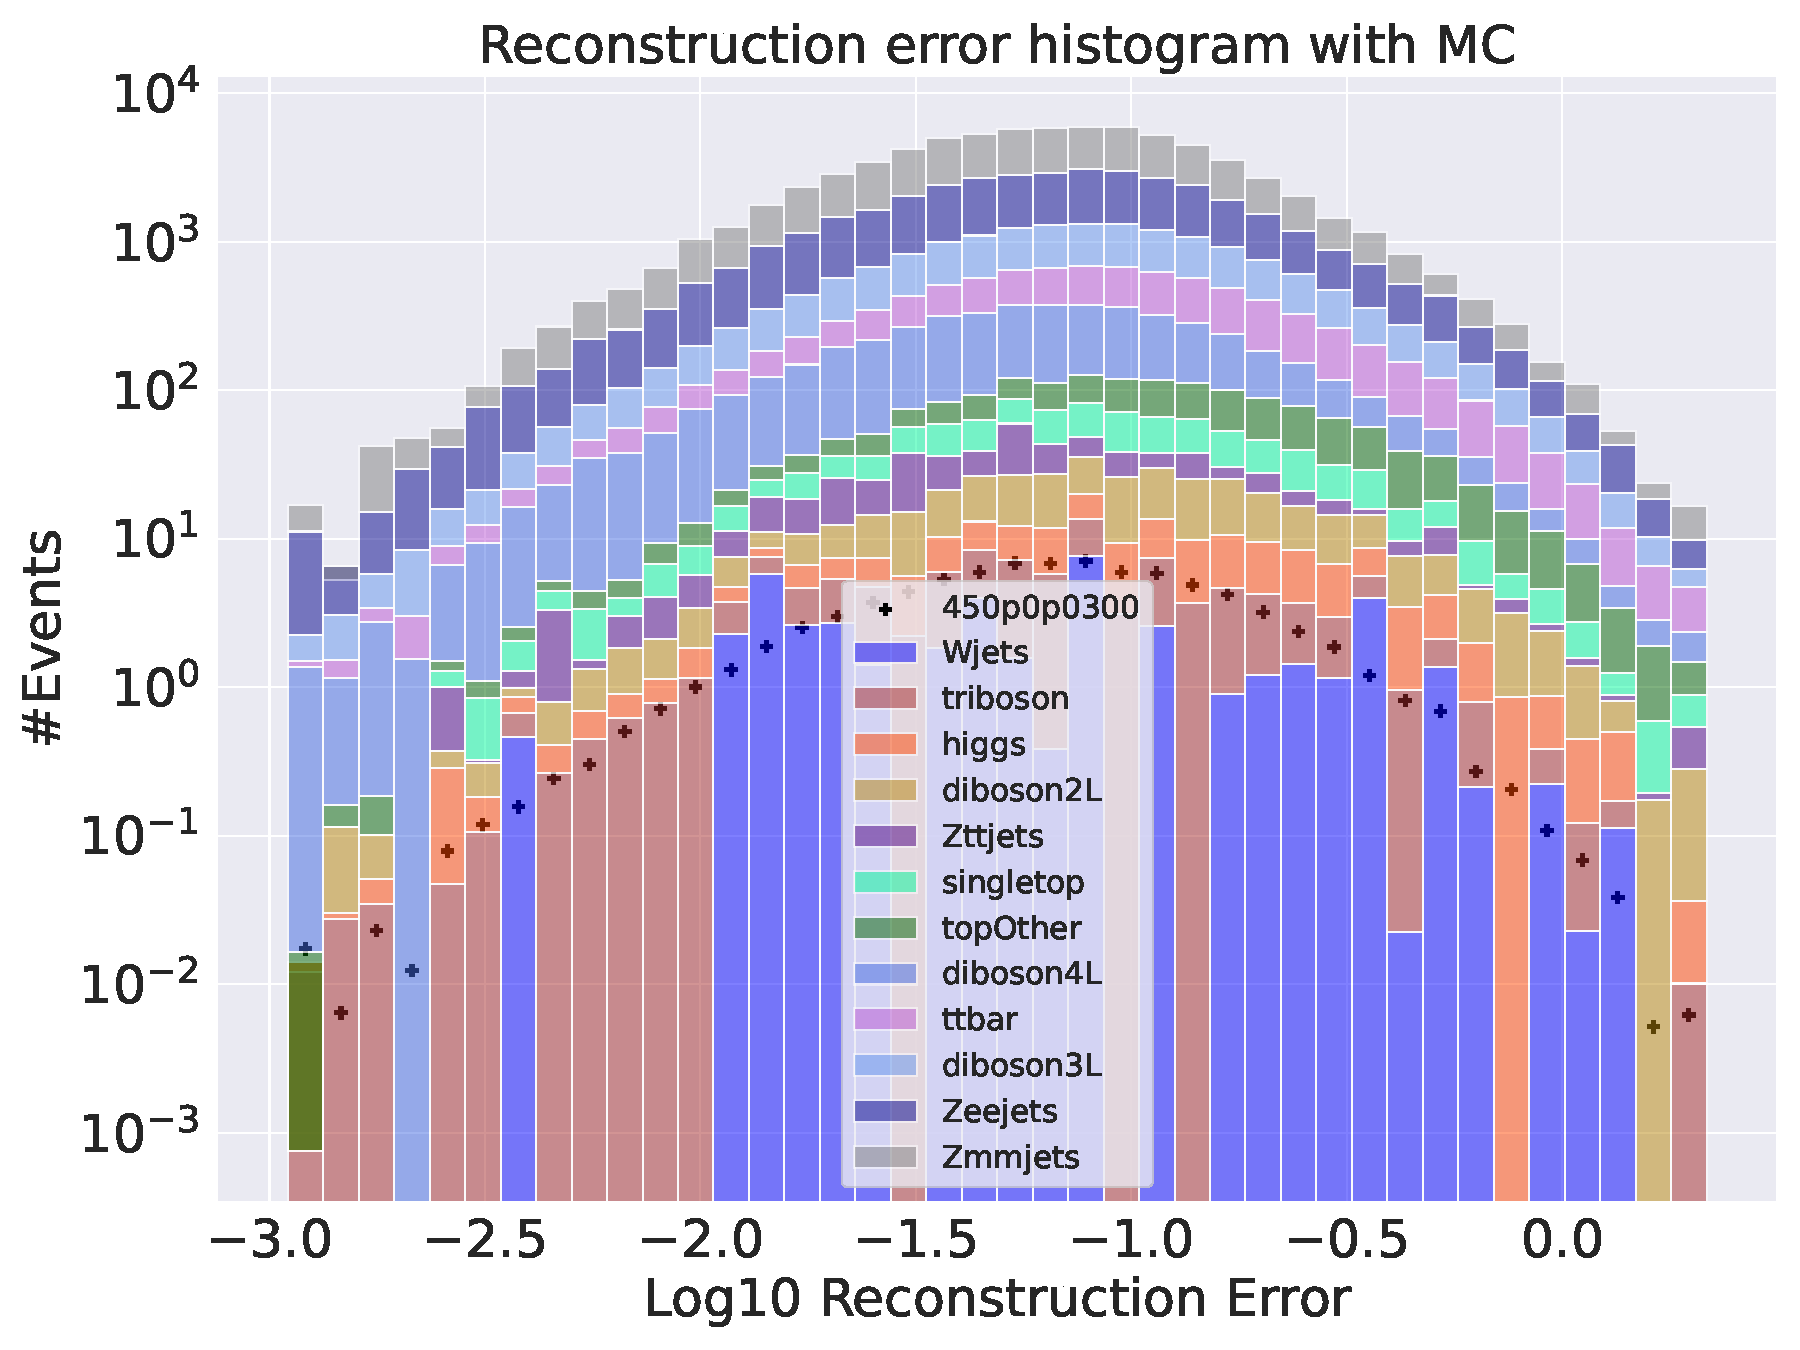
\includegraphics[width=\textwidth]{Figures/VAE_testing/big/3lep/b_data_recon_big_rm3_feats_sig_450p0p0300.pdf}
        \caption{ }
        \label{fig:VAE_3lep_big_450}
    \end{subfigure}
    \hfill
    \begin{subfigure}{.45\textwidth}
        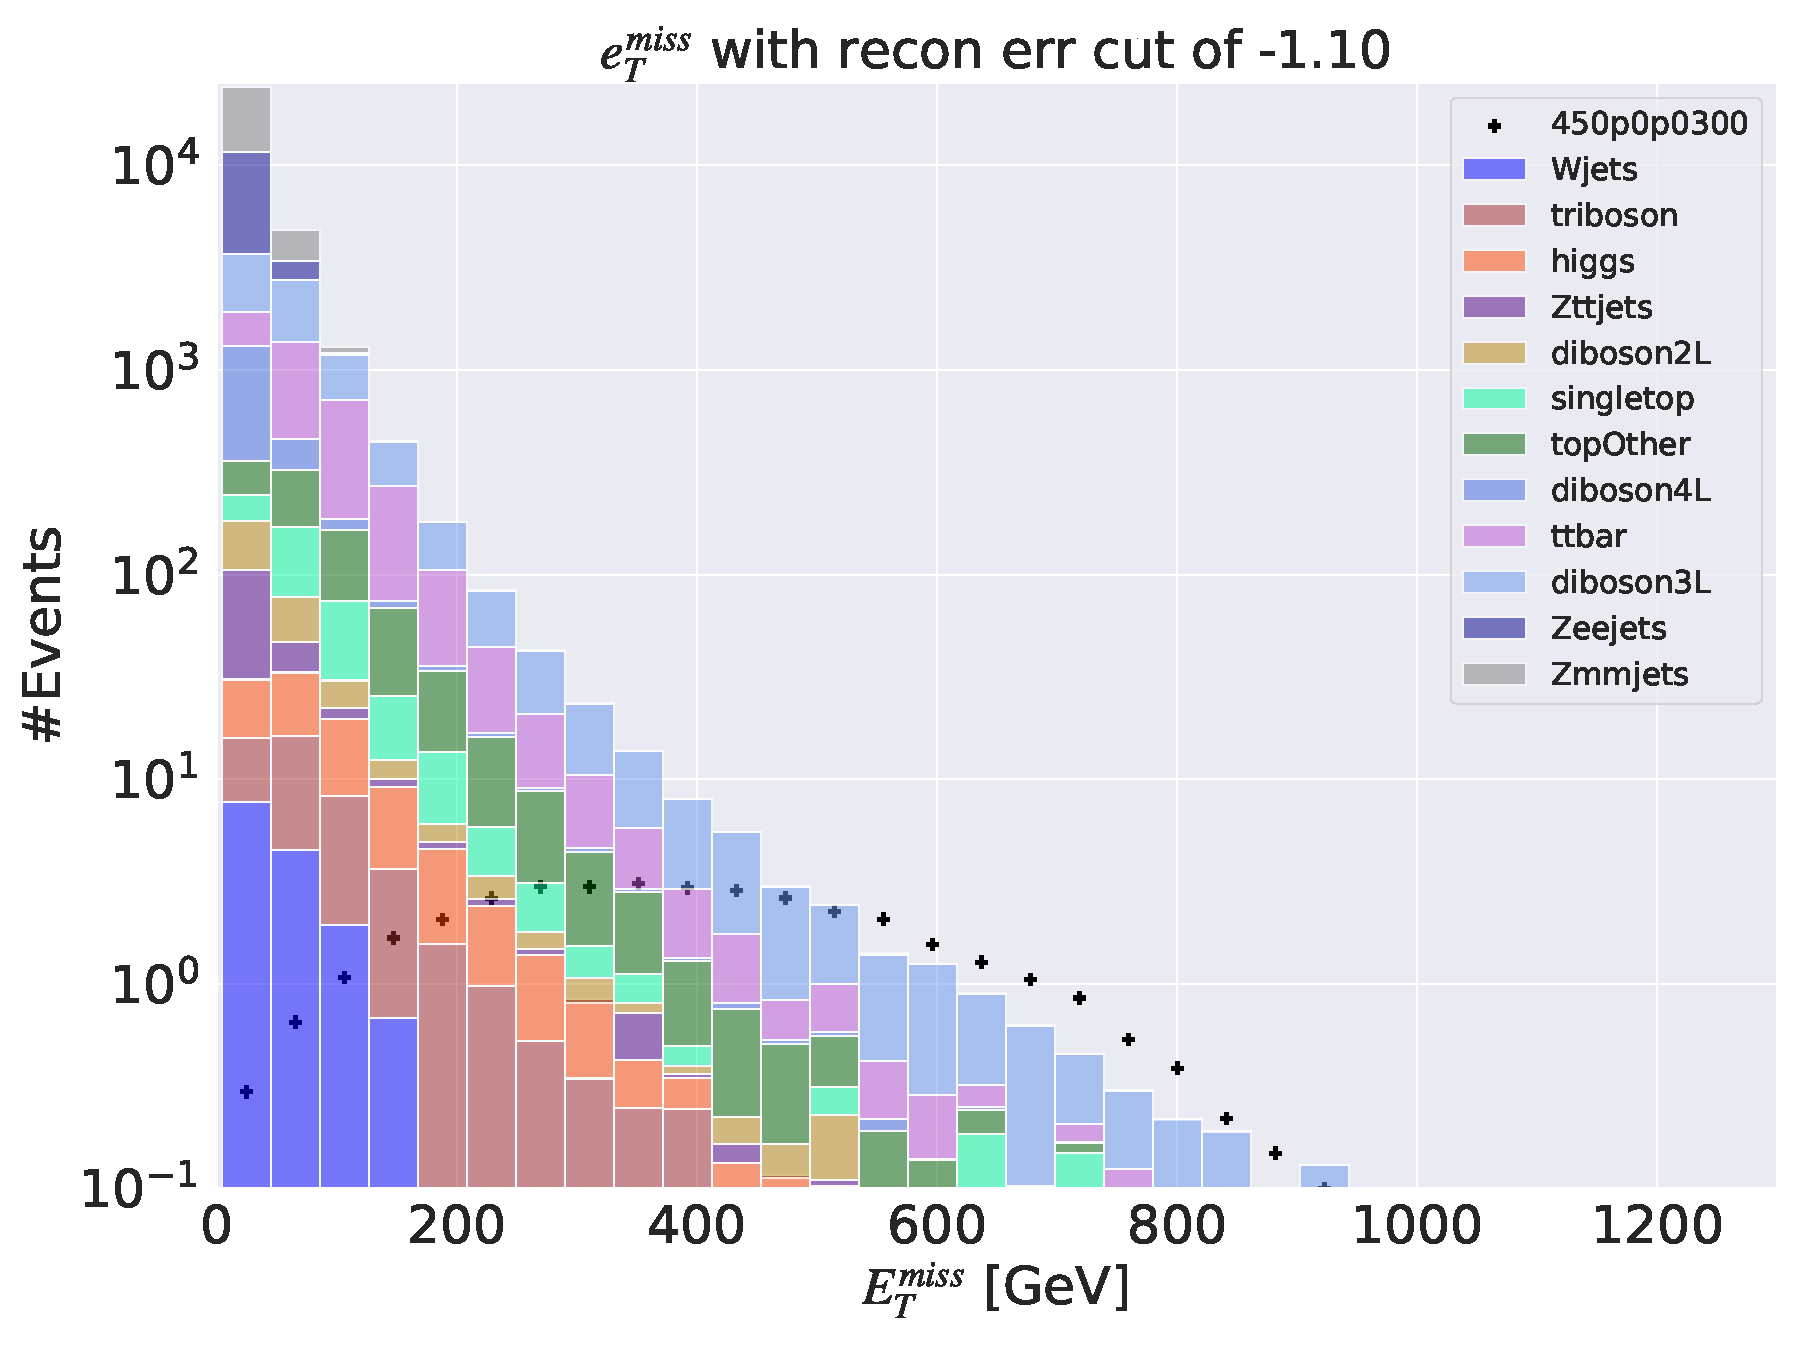
\includegraphics[width=\textwidth]{Figures/VAE_testing/big/3lep/b_data_recon_big_rm3_feats_sig_450p0p0300_etmiss_recon_errcut_-1.10.pdf}
        \caption{}
        \label{fig:VAE_3lep_big_etmiss_450}
    \end{subfigure}
    \hfill
    \begin{subfigure}{.45\textwidth}
        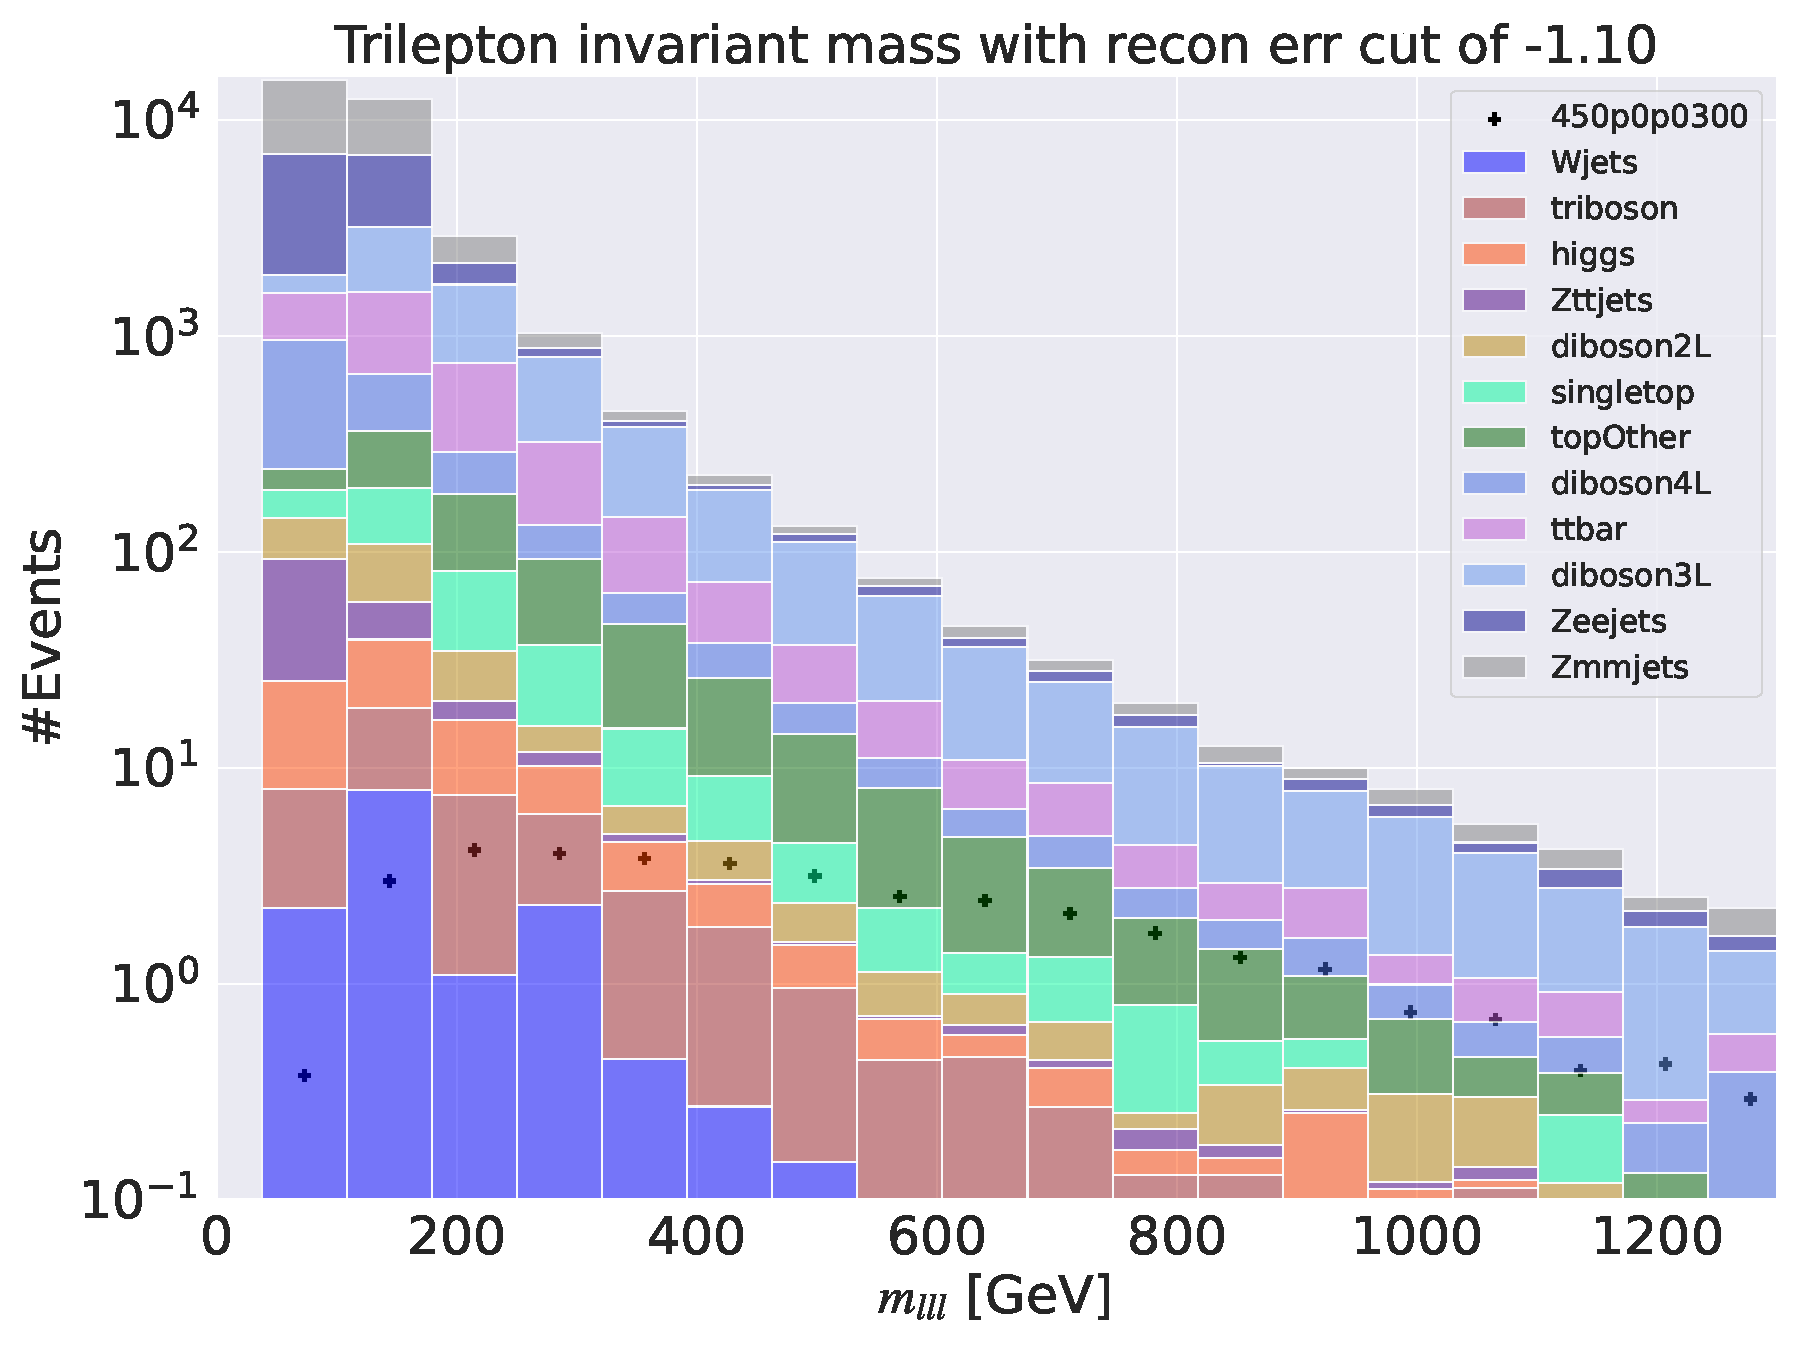
\includegraphics[width=\textwidth]{Figures/VAE_testing/big/3lep/b_data_recon_big_rm3_feats_sig_450p0p0300_mlll_recon_errcut_-1.10.pdf}
        \caption{}
        \label{fig:VAE_3lep_big_mlll_450}
    \end{subfigure}
    \hfill   
    \begin{subfigure}{.45\textwidth}
        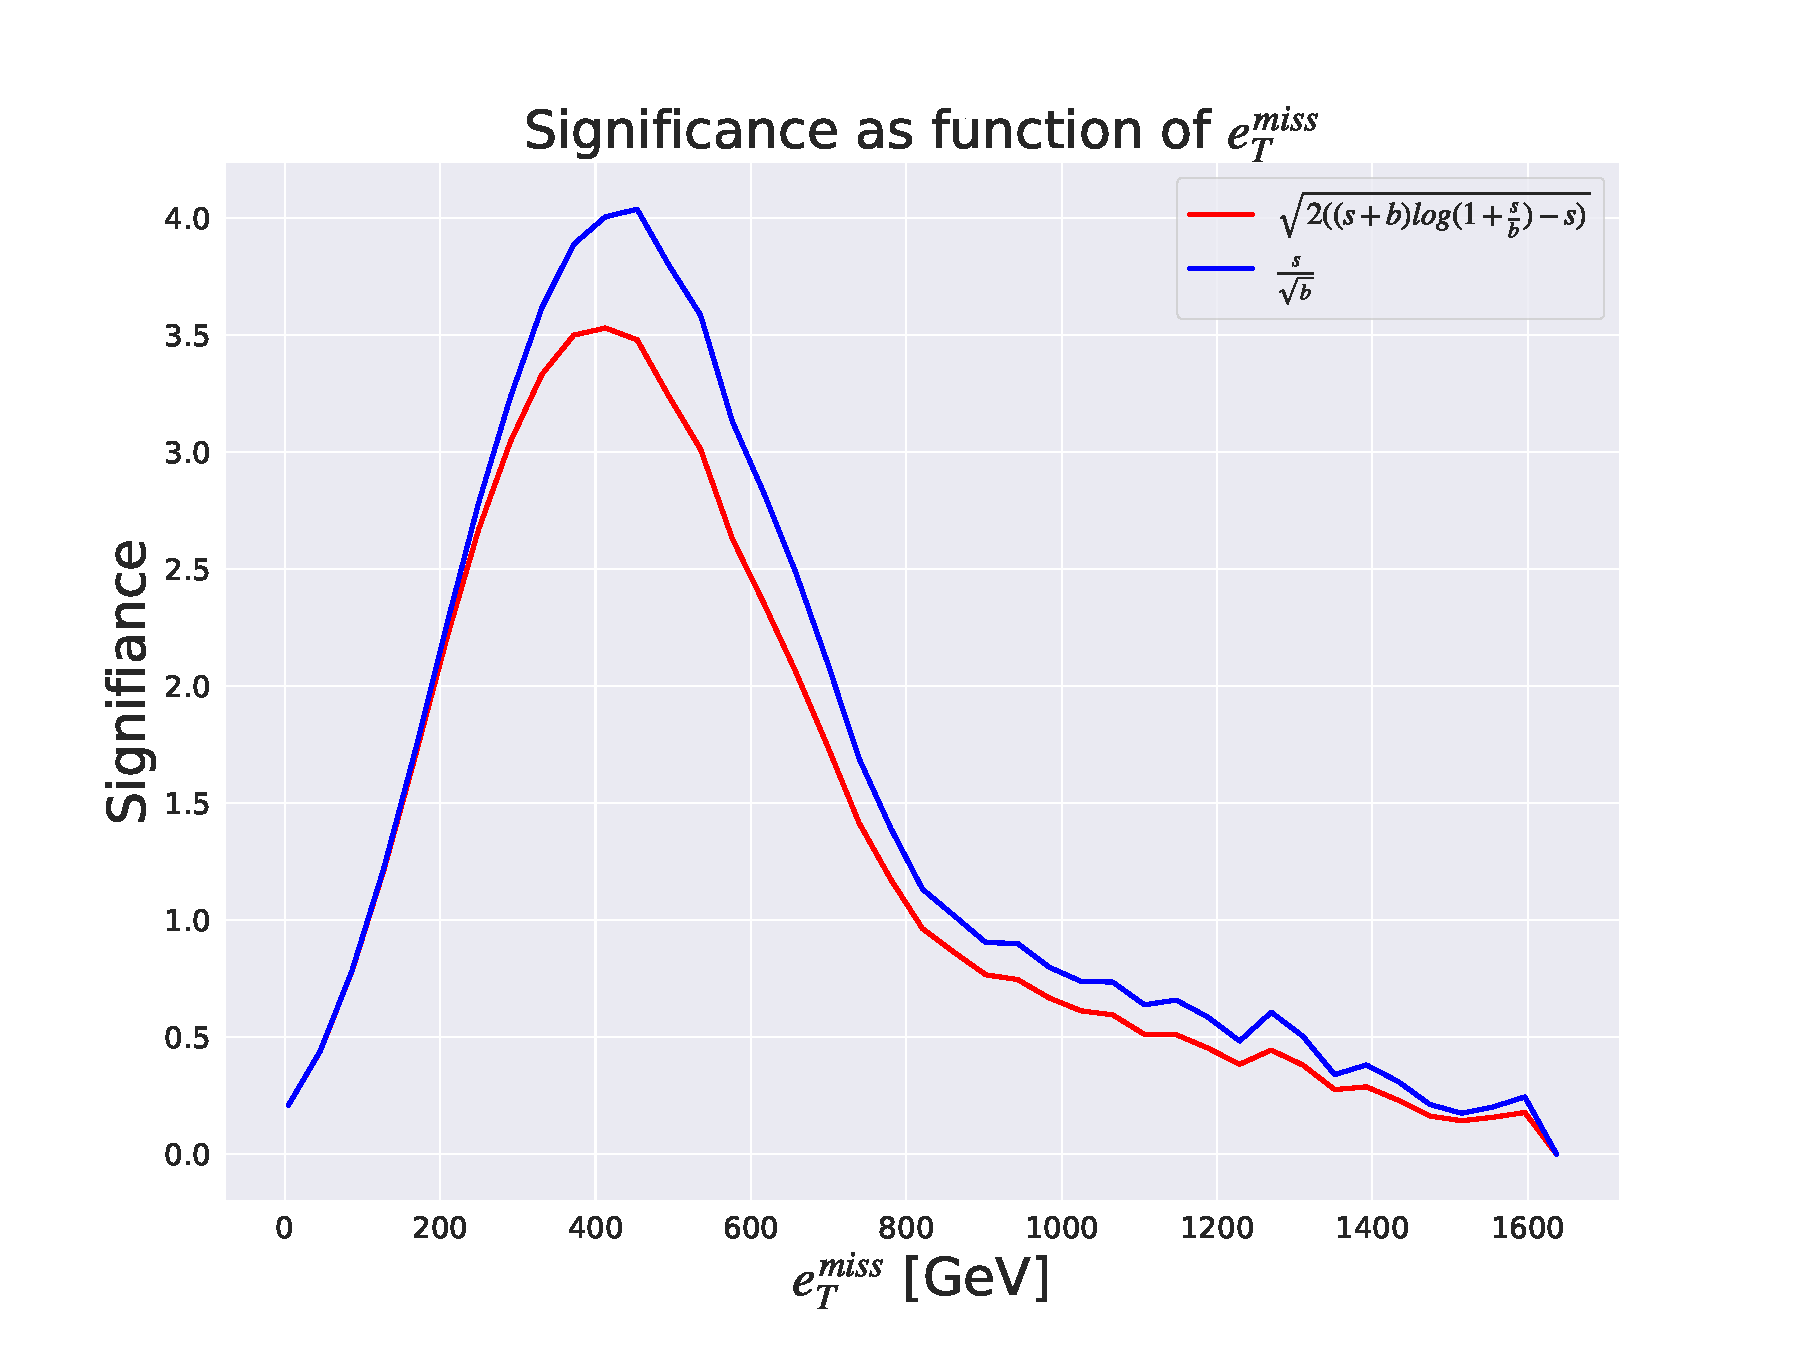
\includegraphics[width=\textwidth]{Figures/VAE_testing/big/3lep/significance_etmiss_450p0p0300_-1.0969148715571329.pdf}
        \caption{}
        \label{fig:VAE_3lep_big_signi_450}
    \end{subfigure}
    \hfill      
    \caption[3lep deep network | $450p300$]{Reconstruction error, $e_T^{miss}$ signal region, $m_{lll}$ signal region and significance as function of 
    $e_T^{miss}$ for the deep regular autoencoder. Here the SUSY $450p300$ model is used.}
    \label{fig:VAE_3lep_big_rec_sig_signi_450}
\end{figure}

\begin{figure}[H]
    \centering
    \begin{subfigure}{.45\textwidth}
        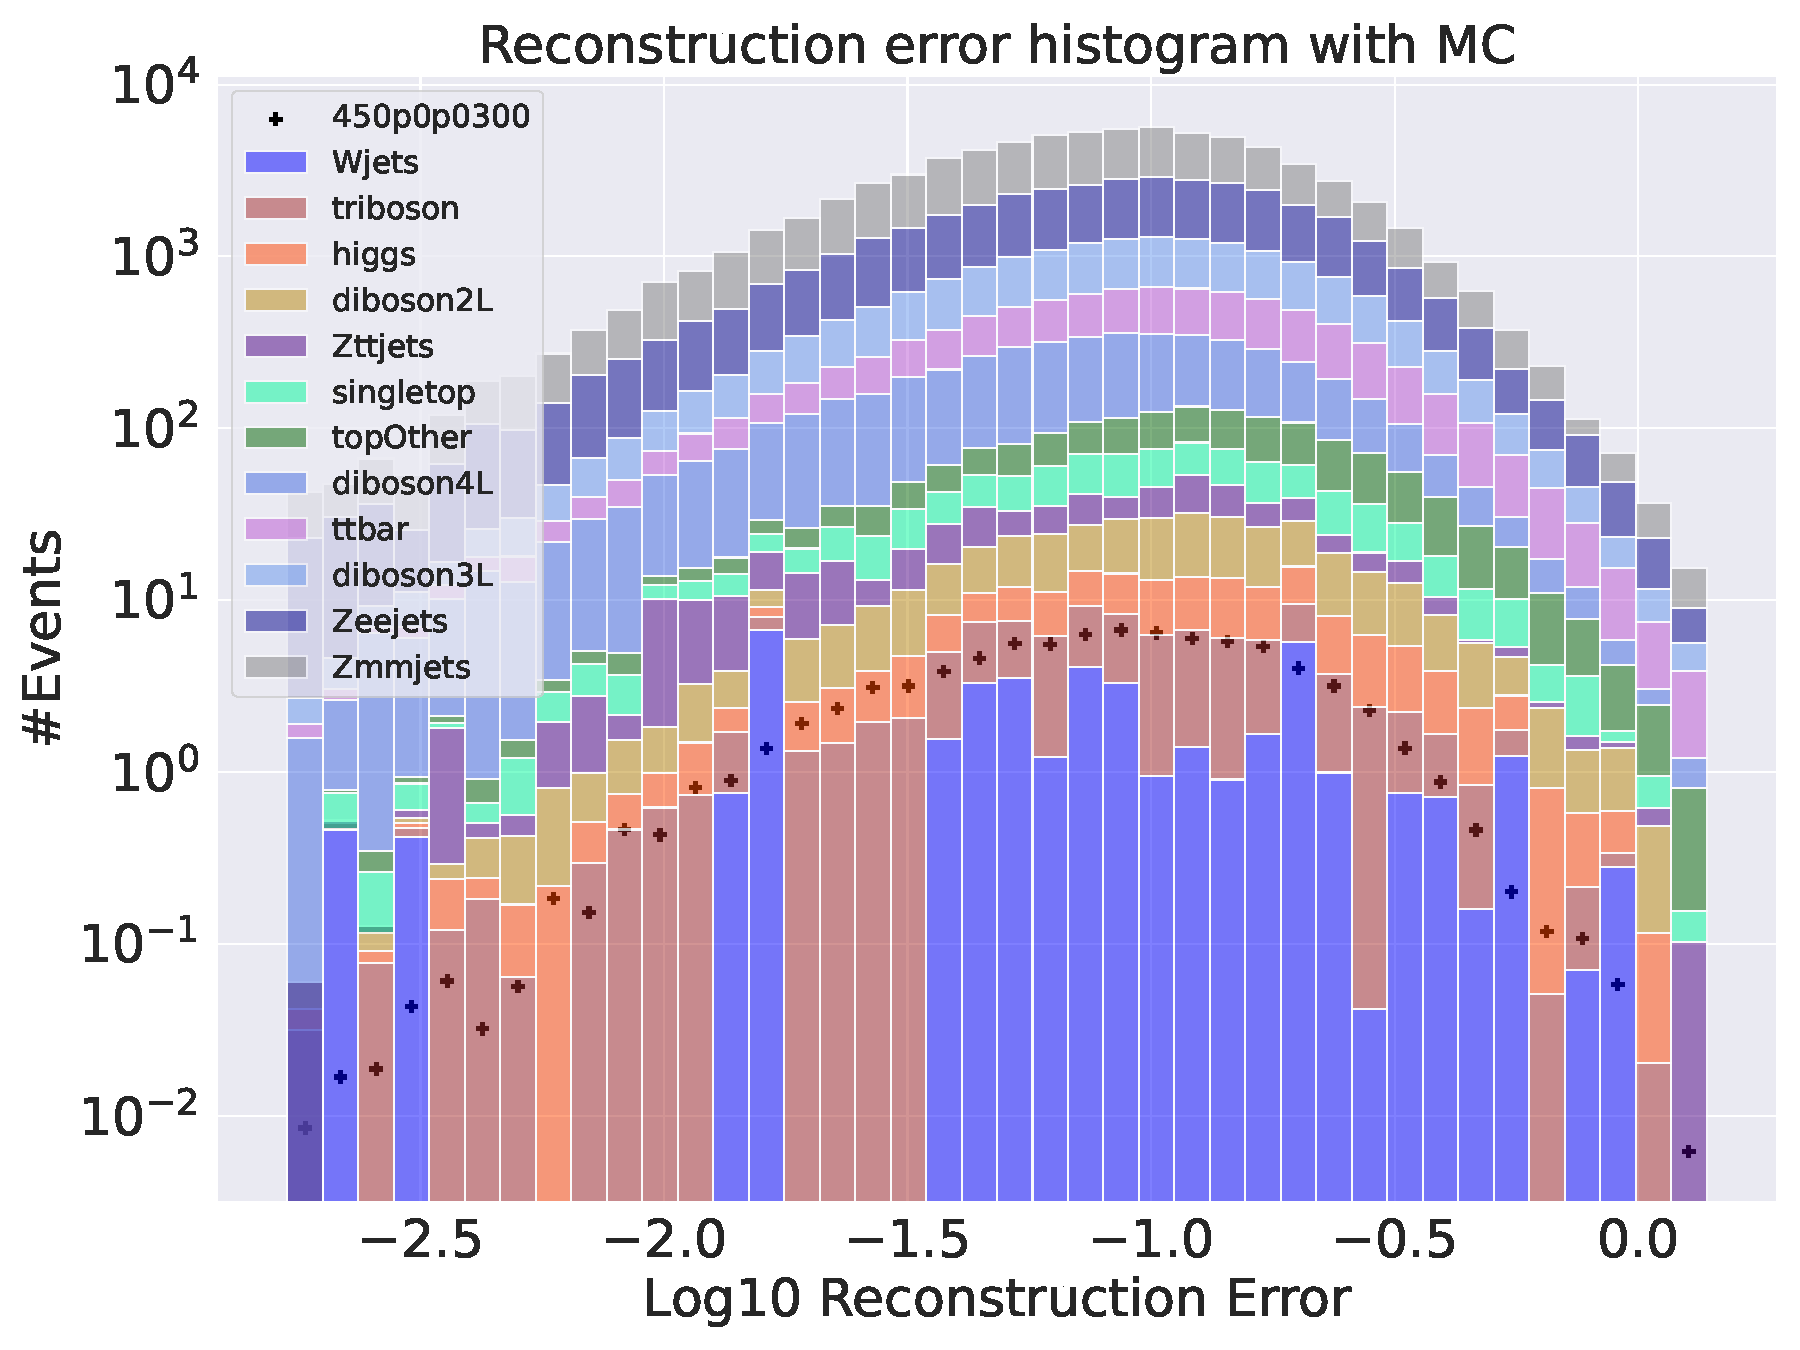
\includegraphics[width=\textwidth]{Figures/VAE_testing/small/3lep/b_data_recon_big_rm3_feats_sig_450p0p0300.pdf}
        \caption{ }
        \label{fig:VAE_3lep_small_450}
    \end{subfigure}
    \hfill
    \begin{subfigure}{.45\textwidth}
        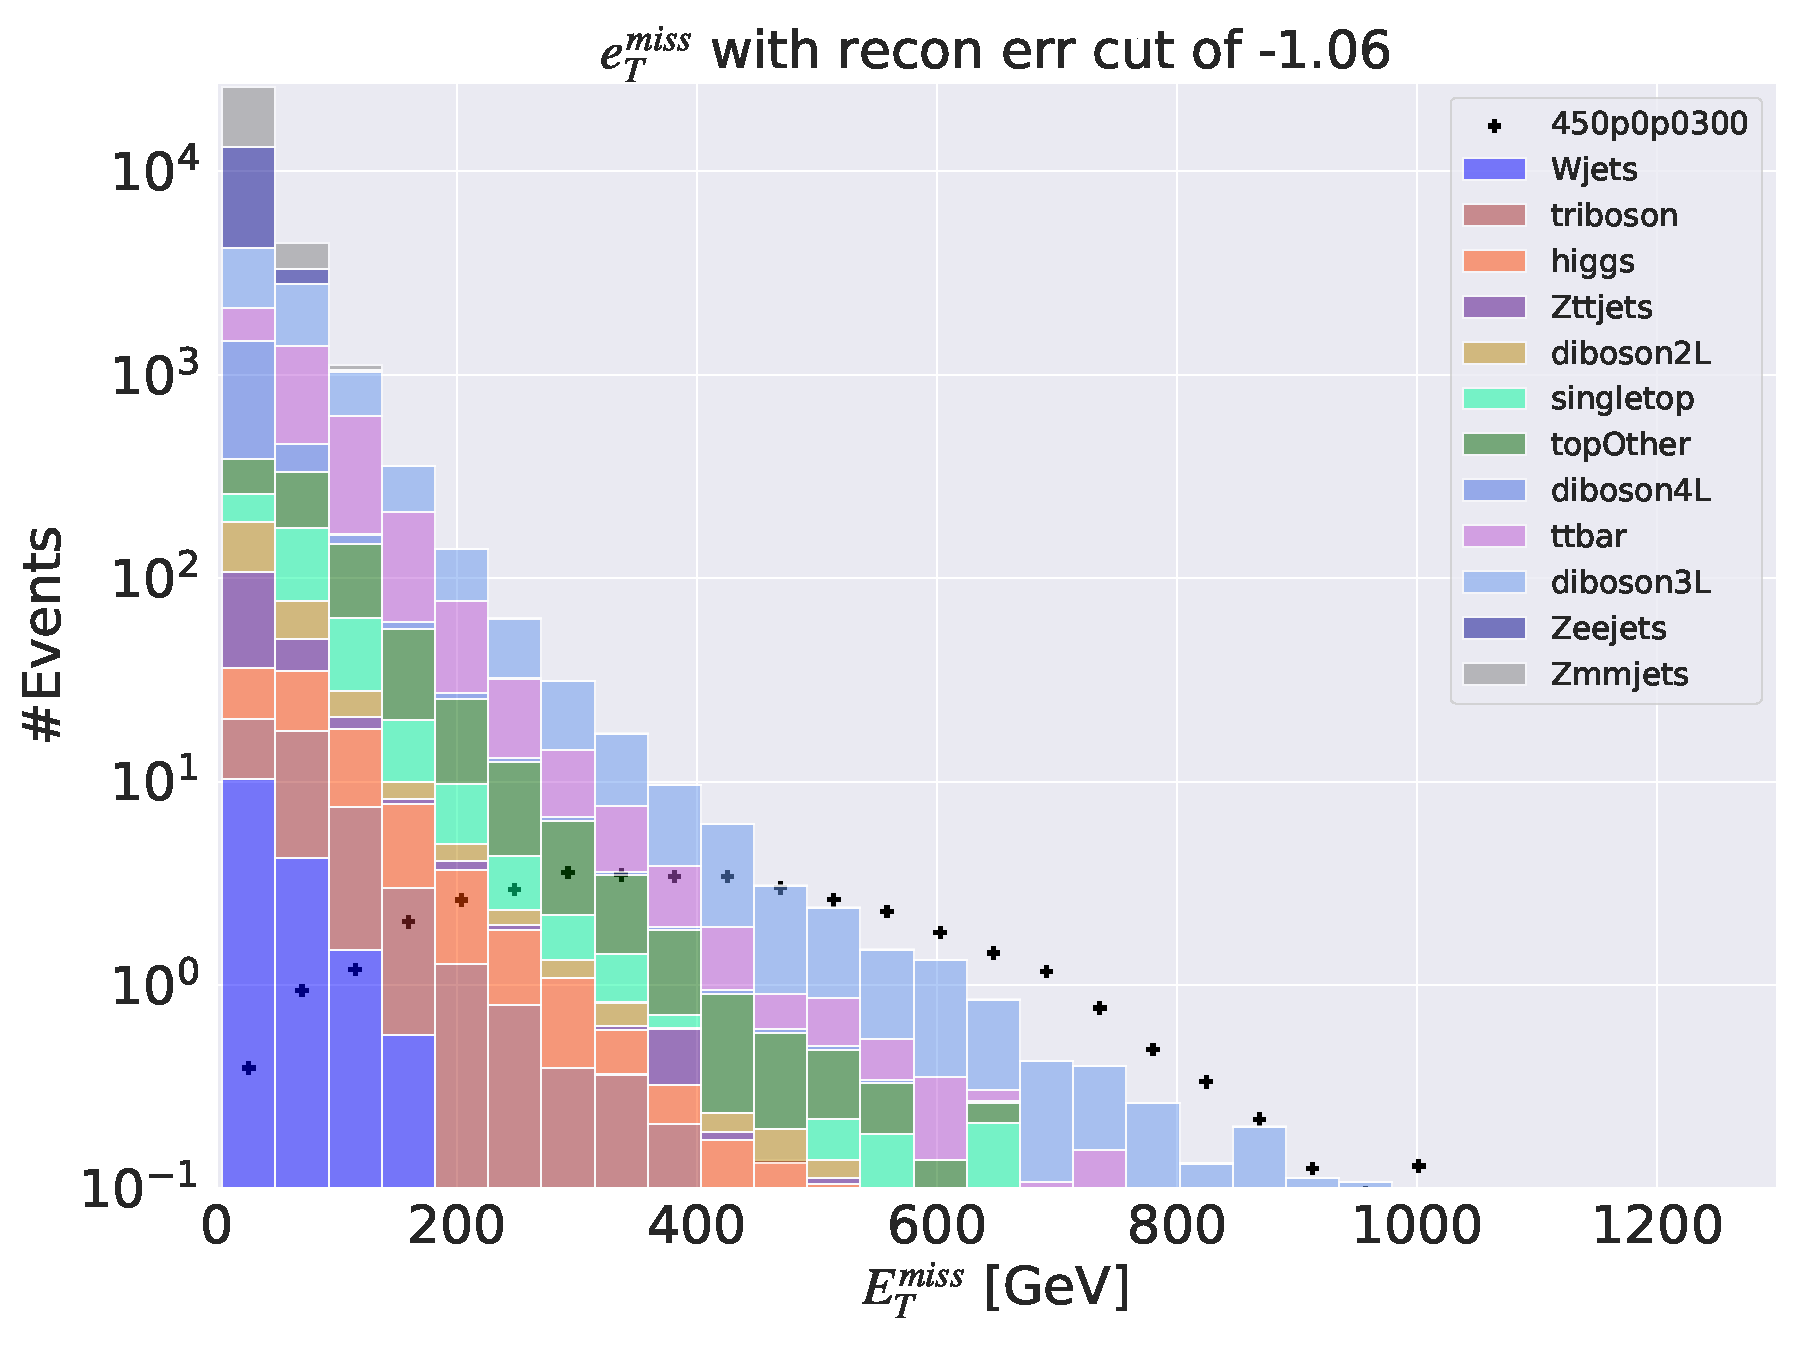
\includegraphics[width=\textwidth]{Figures/VAE_testing/small/3lep/b_data_recon_big_rm3_feats_sig_450p0p0300_etmiss_recon_errcut_-1.06.pdf}
        \caption{}
        \label{fig:VAE_3lep_small_etmiss_450}
    \end{subfigure}
    \hfill
    \begin{subfigure}{.45\textwidth}
        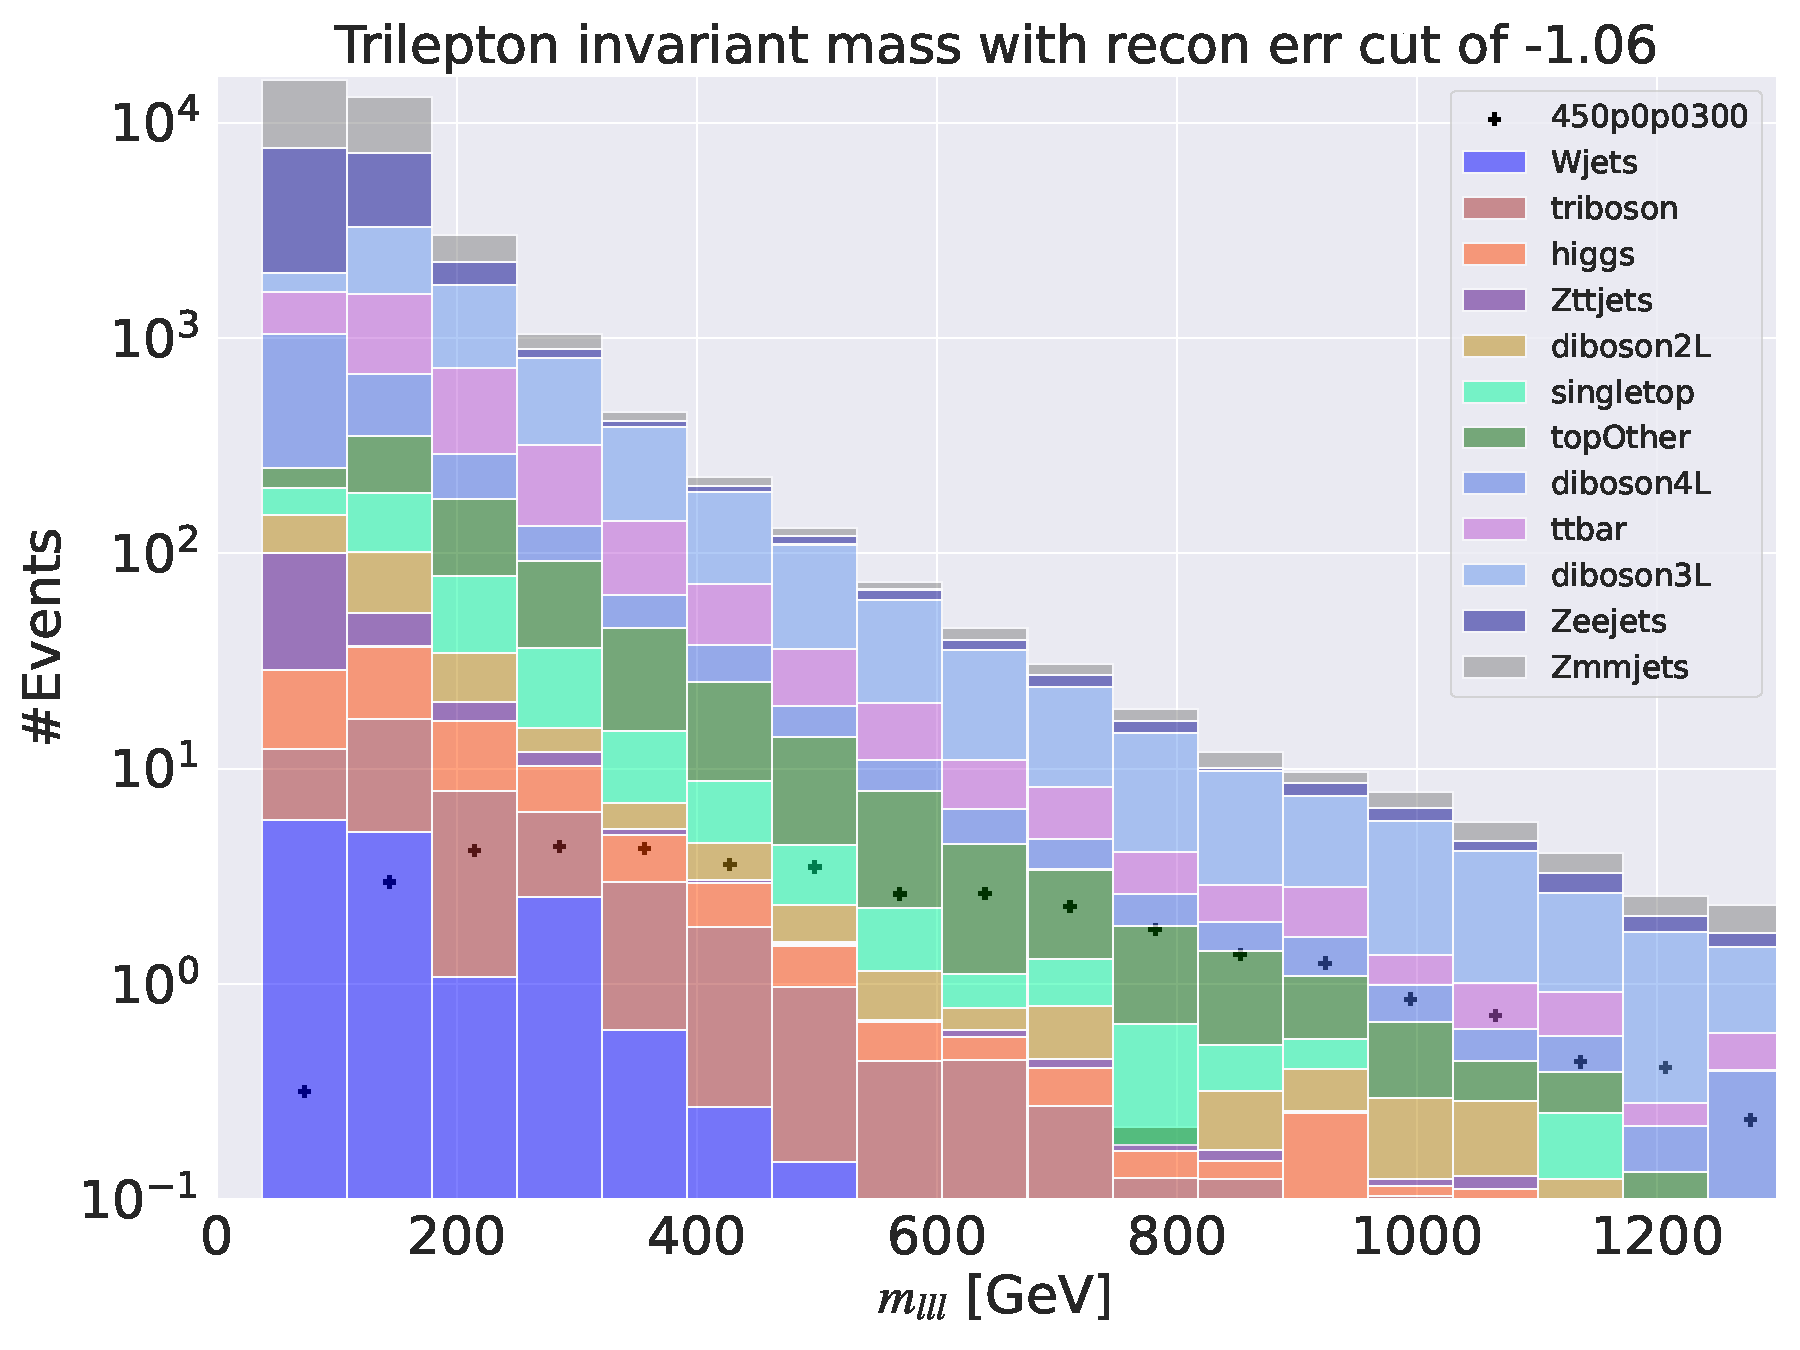
\includegraphics[width=\textwidth]{Figures/VAE_testing/small/3lep/b_data_recon_big_rm3_feats_sig_450p0p0300_mlll_recon_errcut_-1.06.pdf}
        \caption{}
        \label{fig:VAE_3lep_small_mlll_450}
    \end{subfigure}
    \hfill   
    \begin{subfigure}{.45\textwidth}
        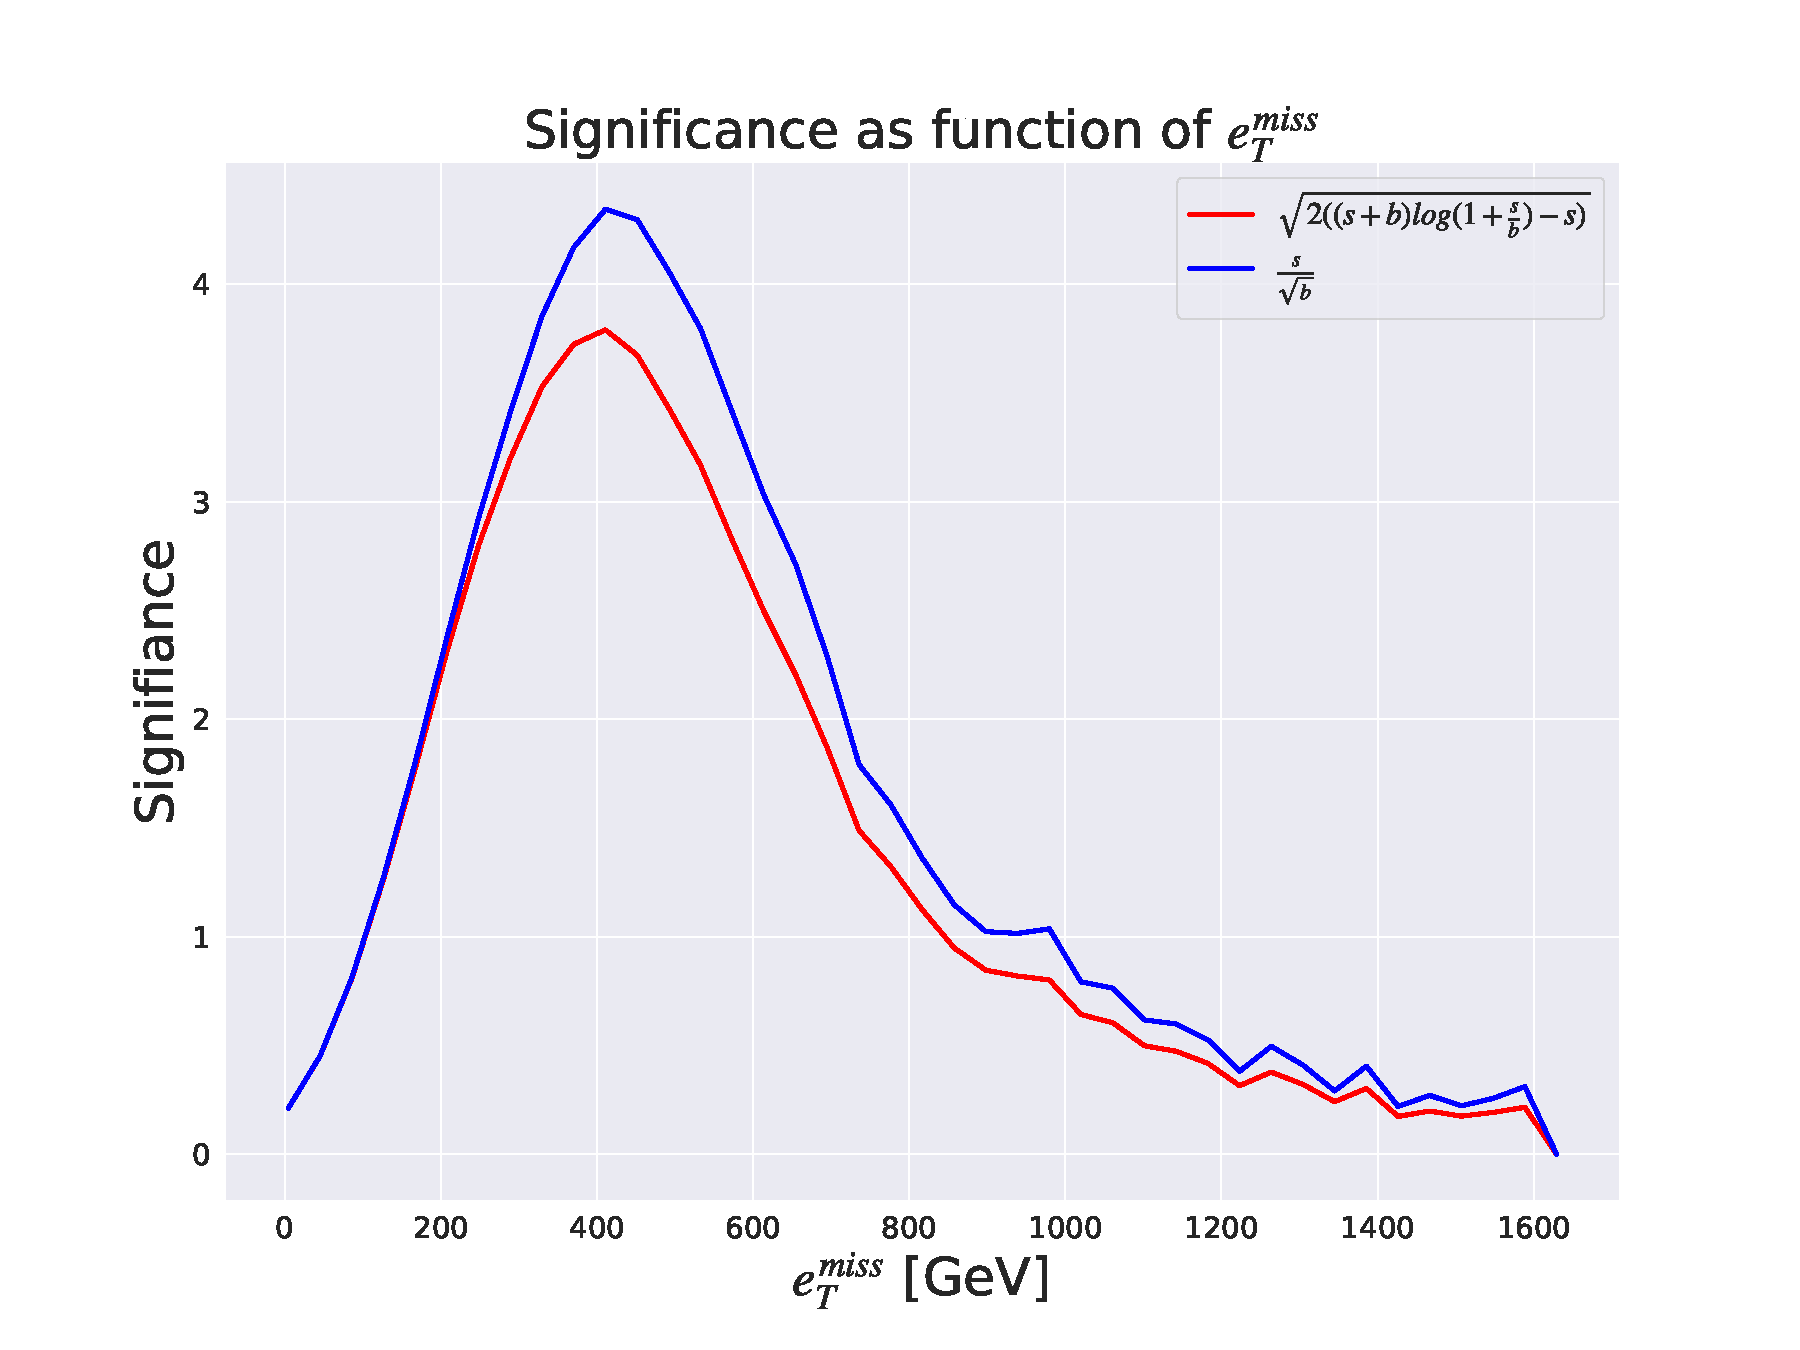
\includegraphics[width=\textwidth]{Figures/VAE_testing/small/3lep/significance_etmiss_450p0p0300_-1.0610372272331543.pdf}
        \caption{}
        \label{ffig:VAE_3lep_small_signi_450}
    \end{subfigure}
    \hfill      
    \caption[3lep shallow network | $450p300$]{Reconstruction error, $e_T^{miss}$ signal region, $m_{lll}$ signal region and significance as function of 
    $e_T^{miss}$ for the shallow regular autoencoder. Here the SUSY $450p300$ model is used.}
    \label{fig:VAE_3lep_small_rec_sig_signi_450}
\end{figure}








\begin{figure}[H]
    \centering
    \begin{subfigure}{.45\textwidth}
        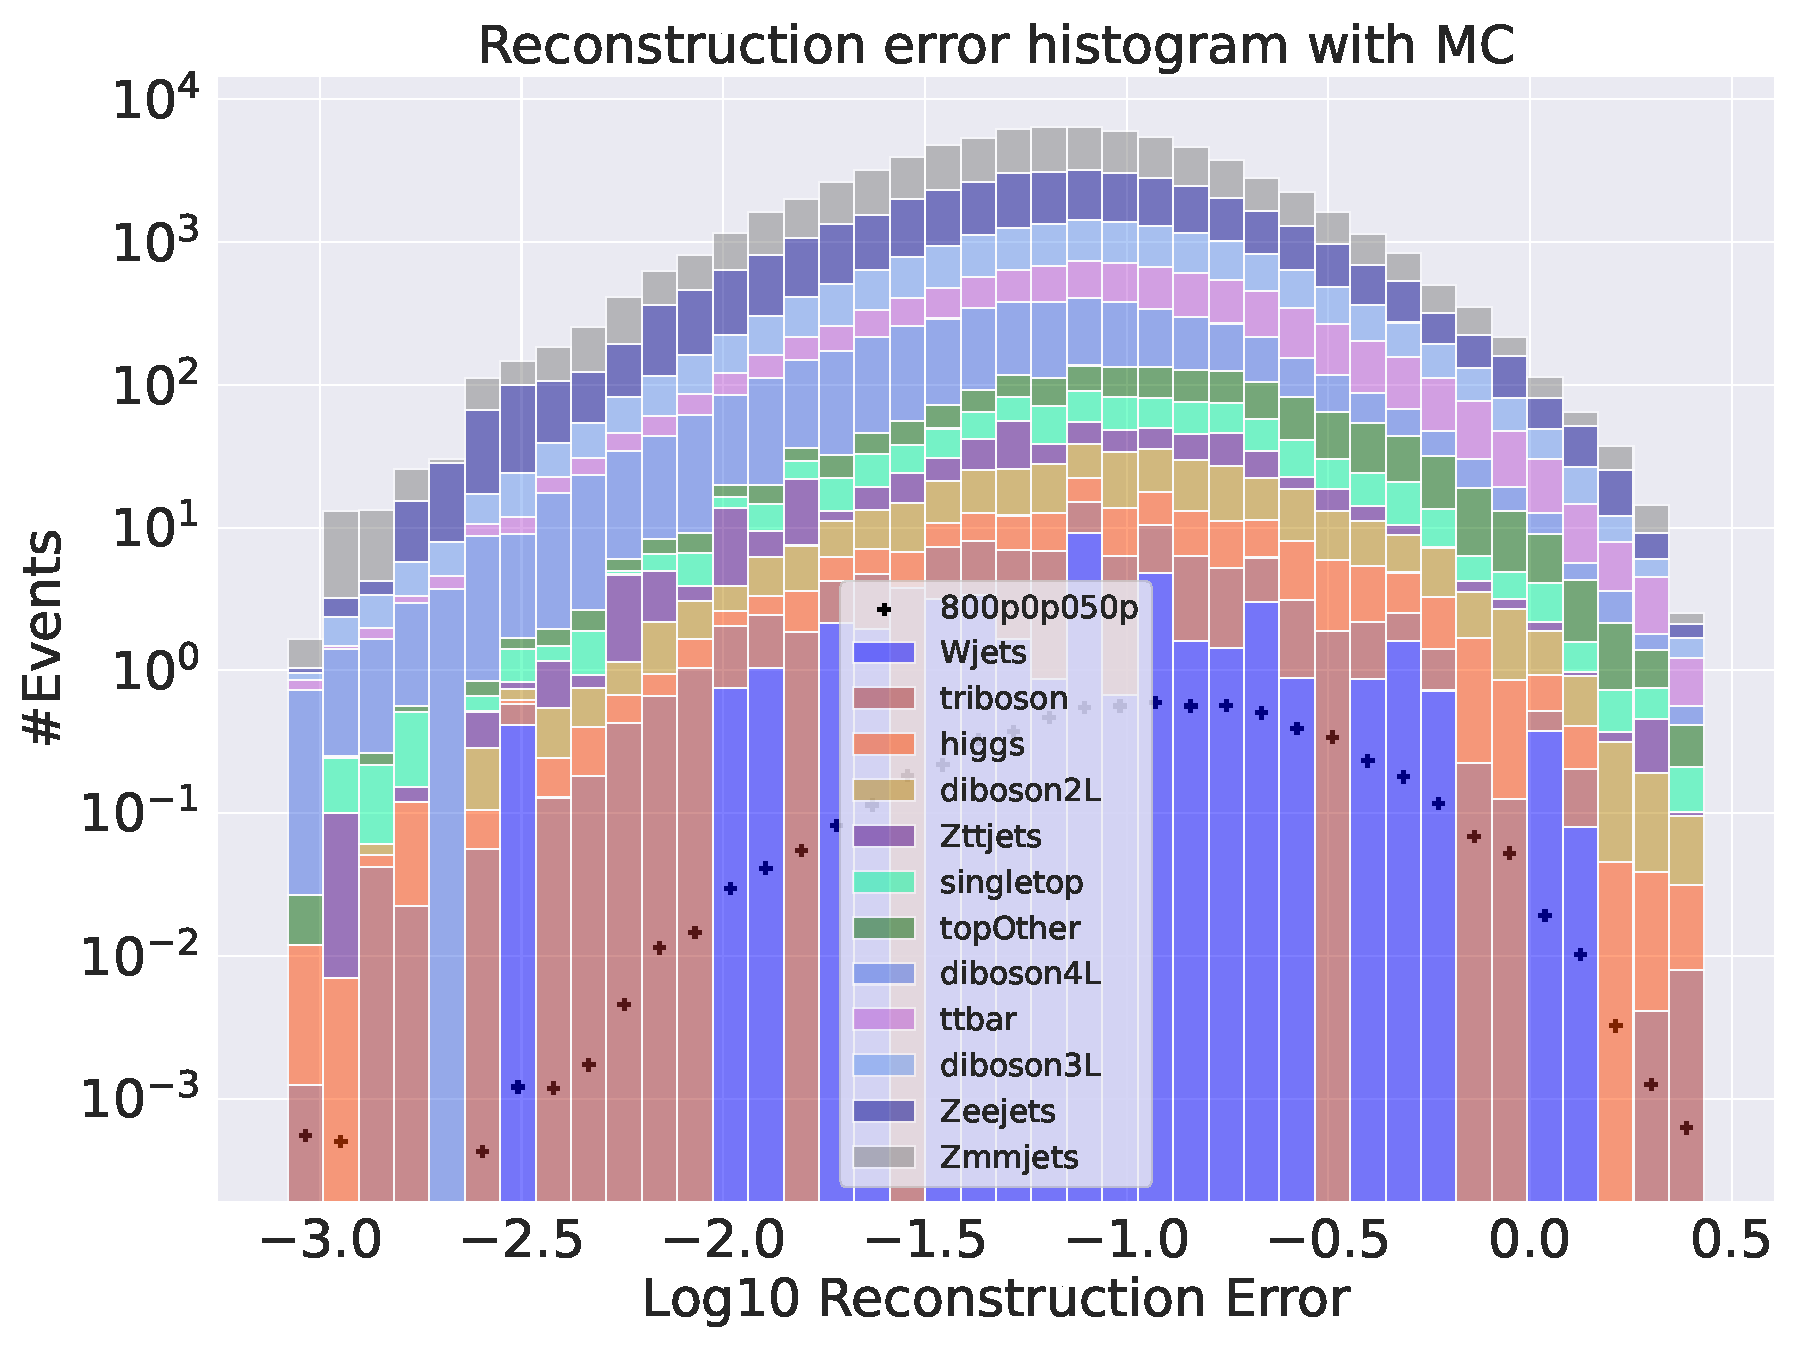
\includegraphics[width=\textwidth]{Figures/VAE_testing/big/3lep/b_data_recon_big_rm3_feats_sig_800p0p050p.pdf}
        \caption{ }
        \label{fig:VAE_3lep_big_800}
    \end{subfigure}
    \hfill
    \begin{subfigure}{.45\textwidth}
        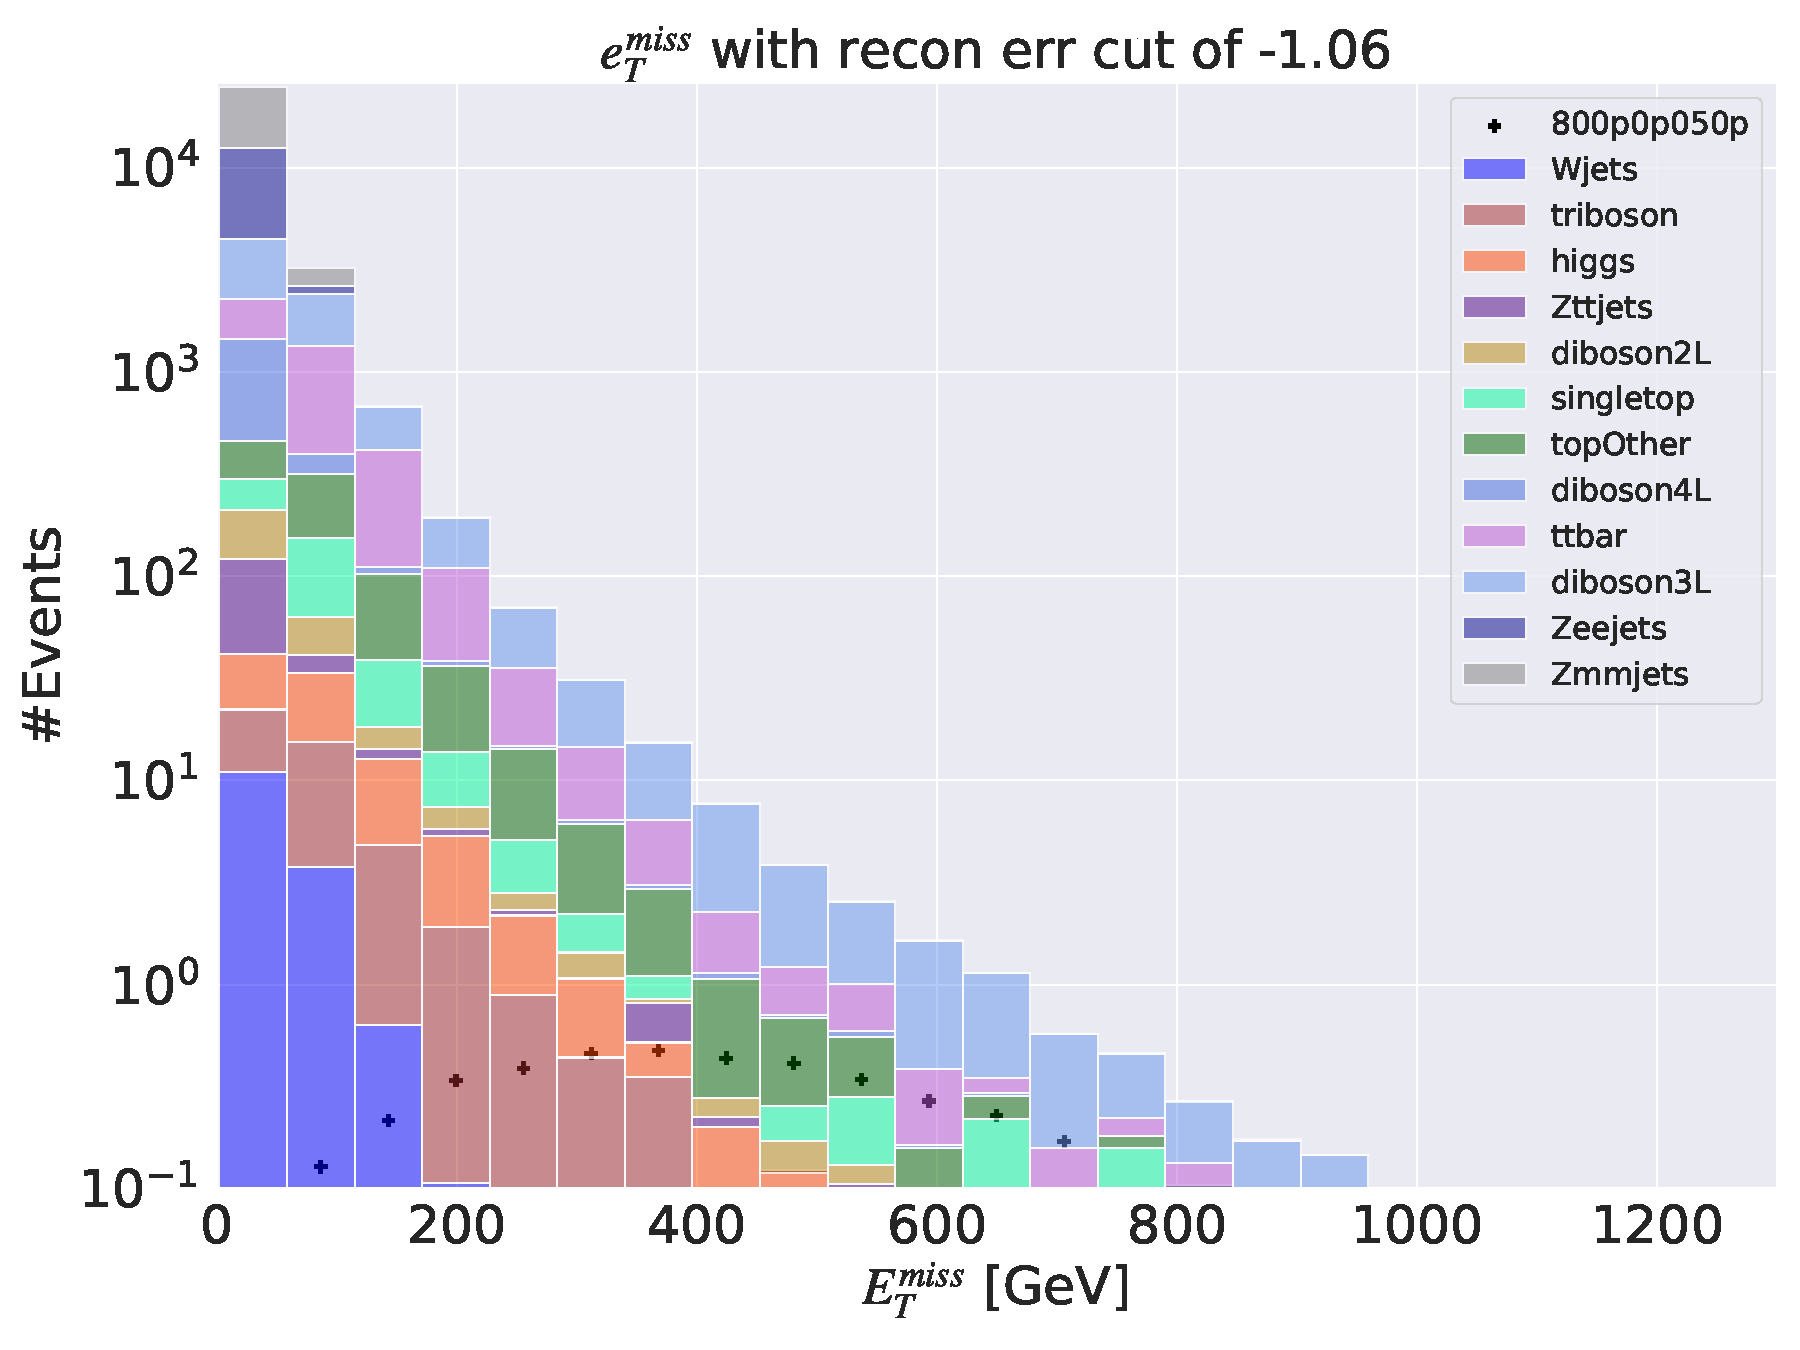
\includegraphics[width=\textwidth]{Figures/VAE_testing/big/3lep/b_data_recon_big_rm3_feats_sig_800p0p050p_etmiss_recon_errcut_-1.06.pdf}
        \caption{}
        \label{fig:VAE_3lep_big_etmiss_800}
    \end{subfigure}
    \hfill
    \begin{subfigure}{.45\textwidth}
        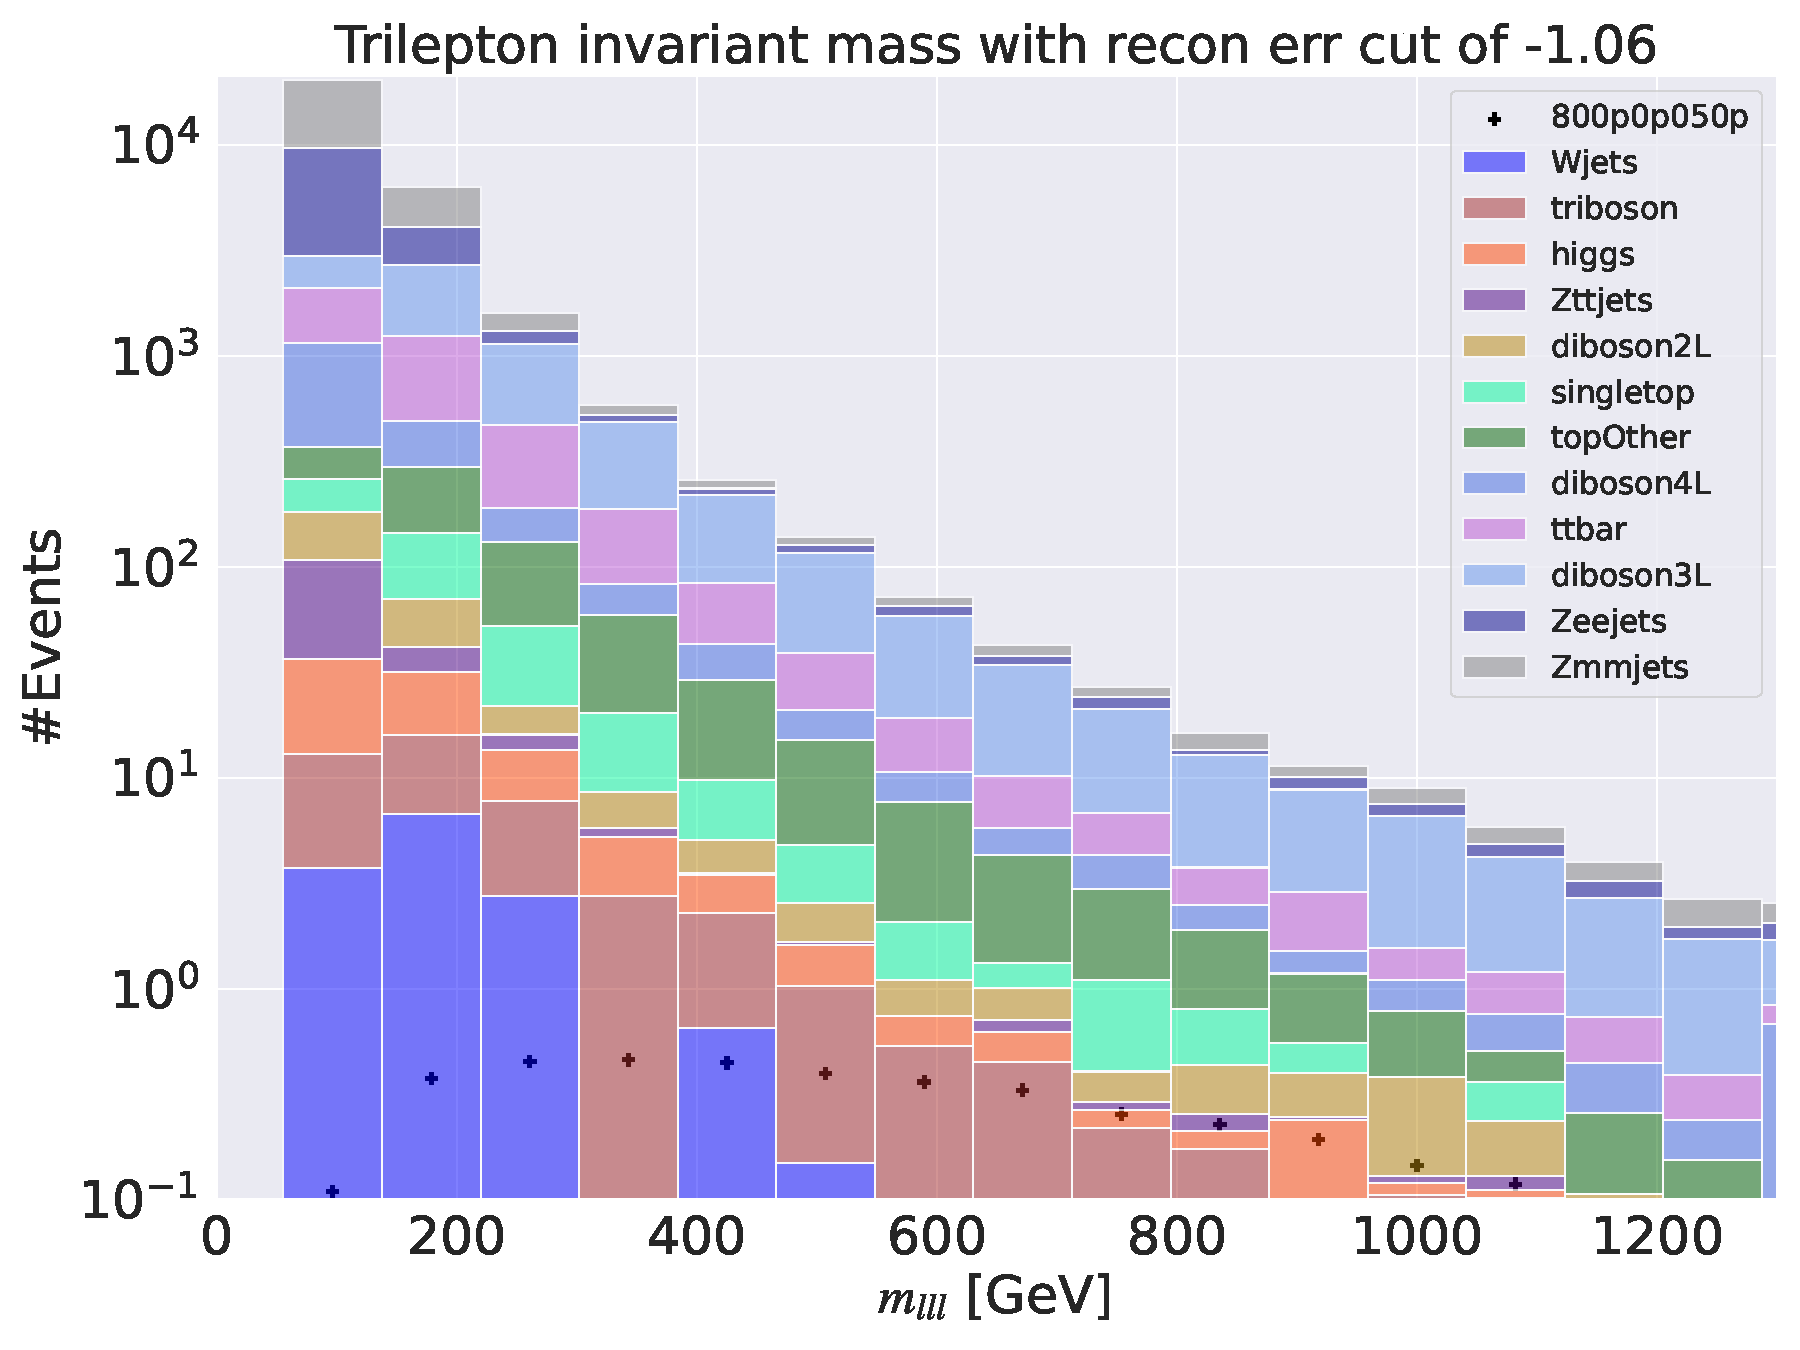
\includegraphics[width=\textwidth]{Figures/VAE_testing/big/3lep/b_data_recon_big_rm3_feats_sig_800p0p050p_mlll_recon_errcut_-1.06.pdf}
        \caption{}
        \label{fig:VAE_3lep_big_mlll_800}
    \end{subfigure}
    \hfill   
    \begin{subfigure}{.45\textwidth}
        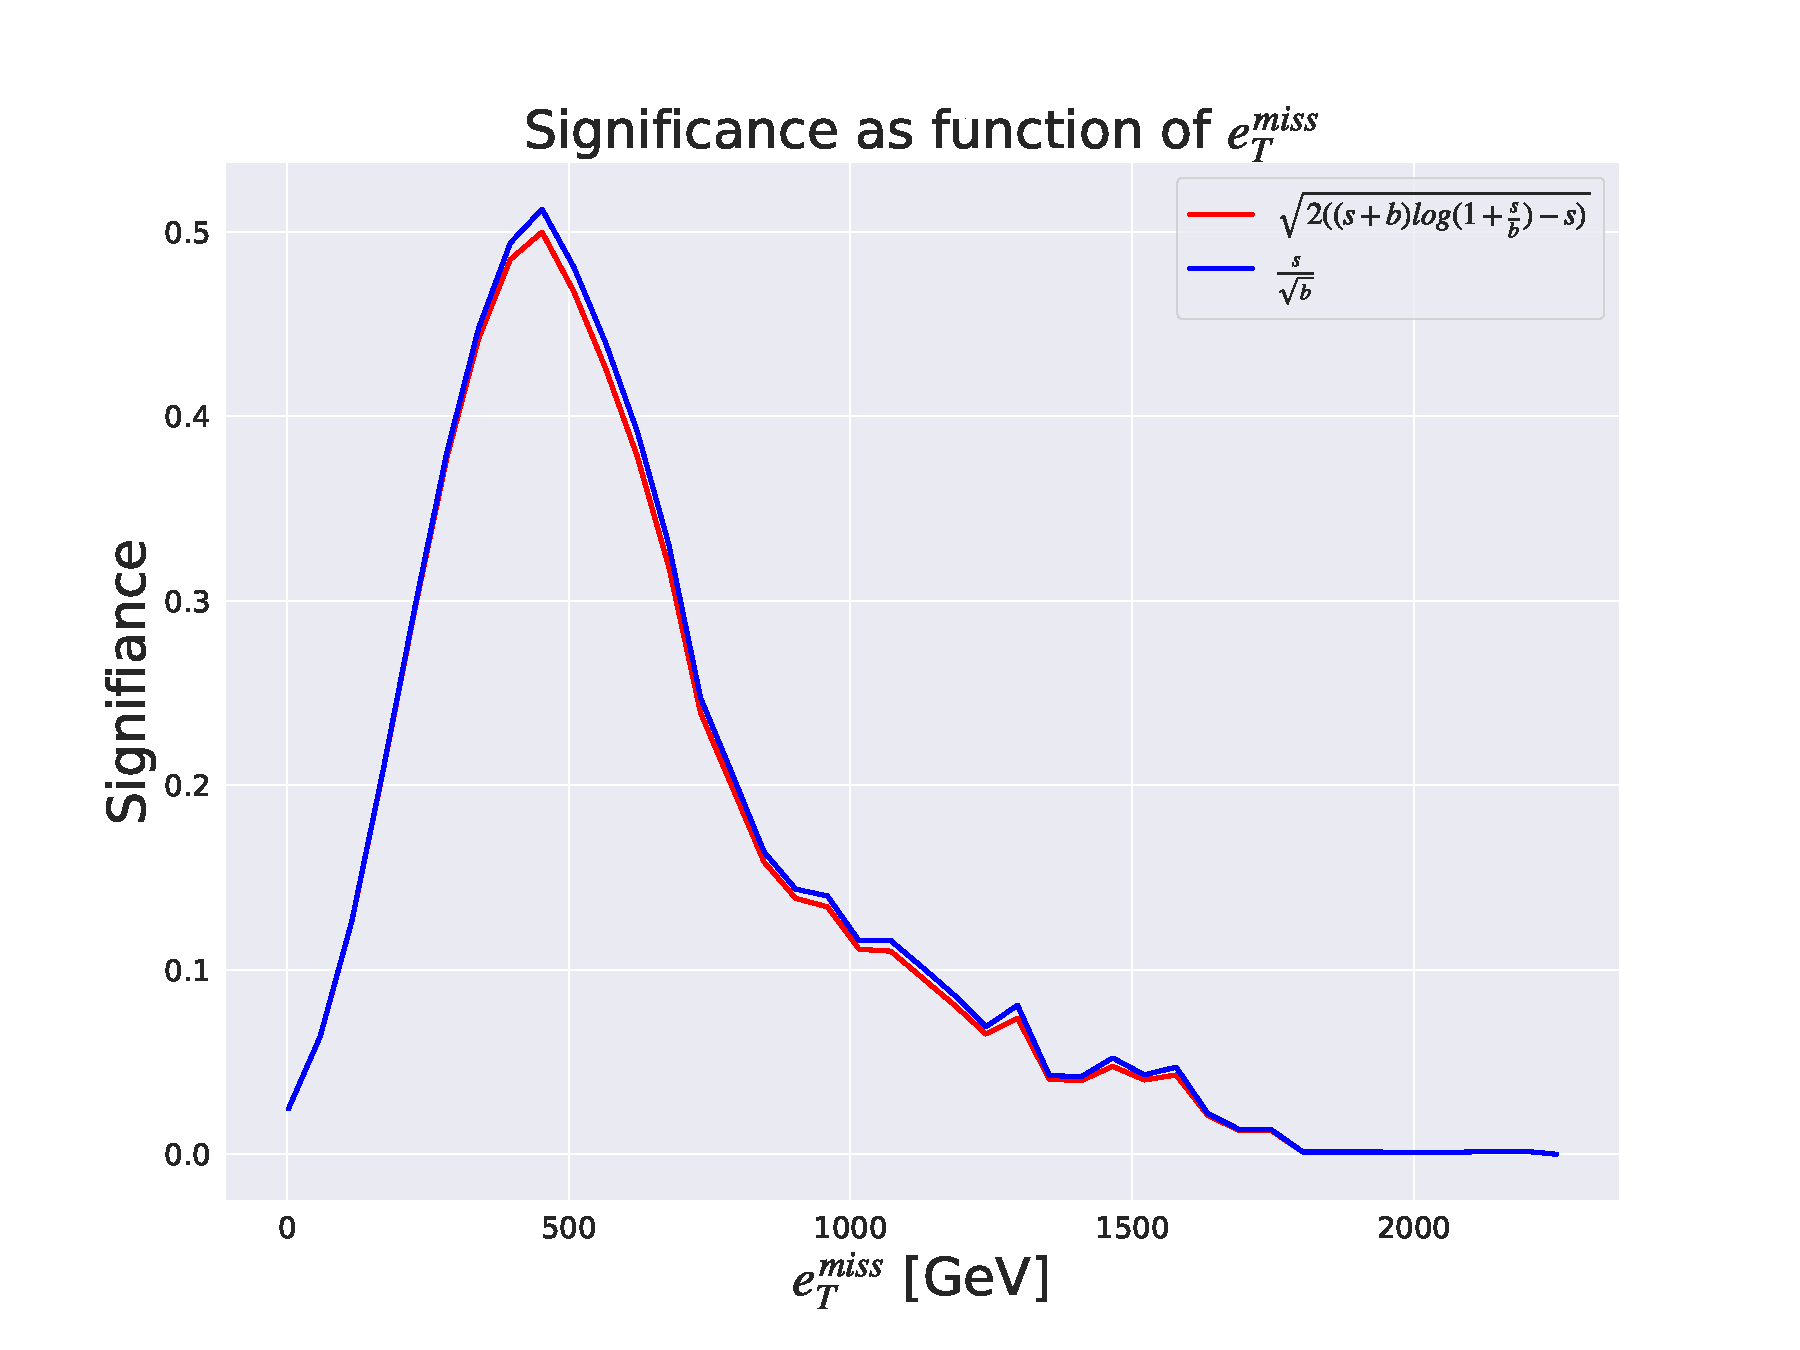
\includegraphics[width=\textwidth]{Figures/VAE_testing/big/3lep/significance_etmiss_800p0p050p_-1.0588523538160817.pdf}
        \caption{}
        \label{fig:VAE_3lep_big_signi_800}
    \end{subfigure}
    \hfill      
    \caption[3lep deep network | $800p50$]{Reconstruction error, $e_T^{miss}$ signal region, $m_{lll}$ signal region and significance as function of 
    $e_T^{miss}$ for the deep regular autoencoder. Here the SUSY $450p300$ model is used.}
    \label{fig:VAE_3lep_big_rec_sig_signi_800}
\end{figure}

\begin{figure}[H]
    \centering
    \begin{subfigure}{.45\textwidth}
        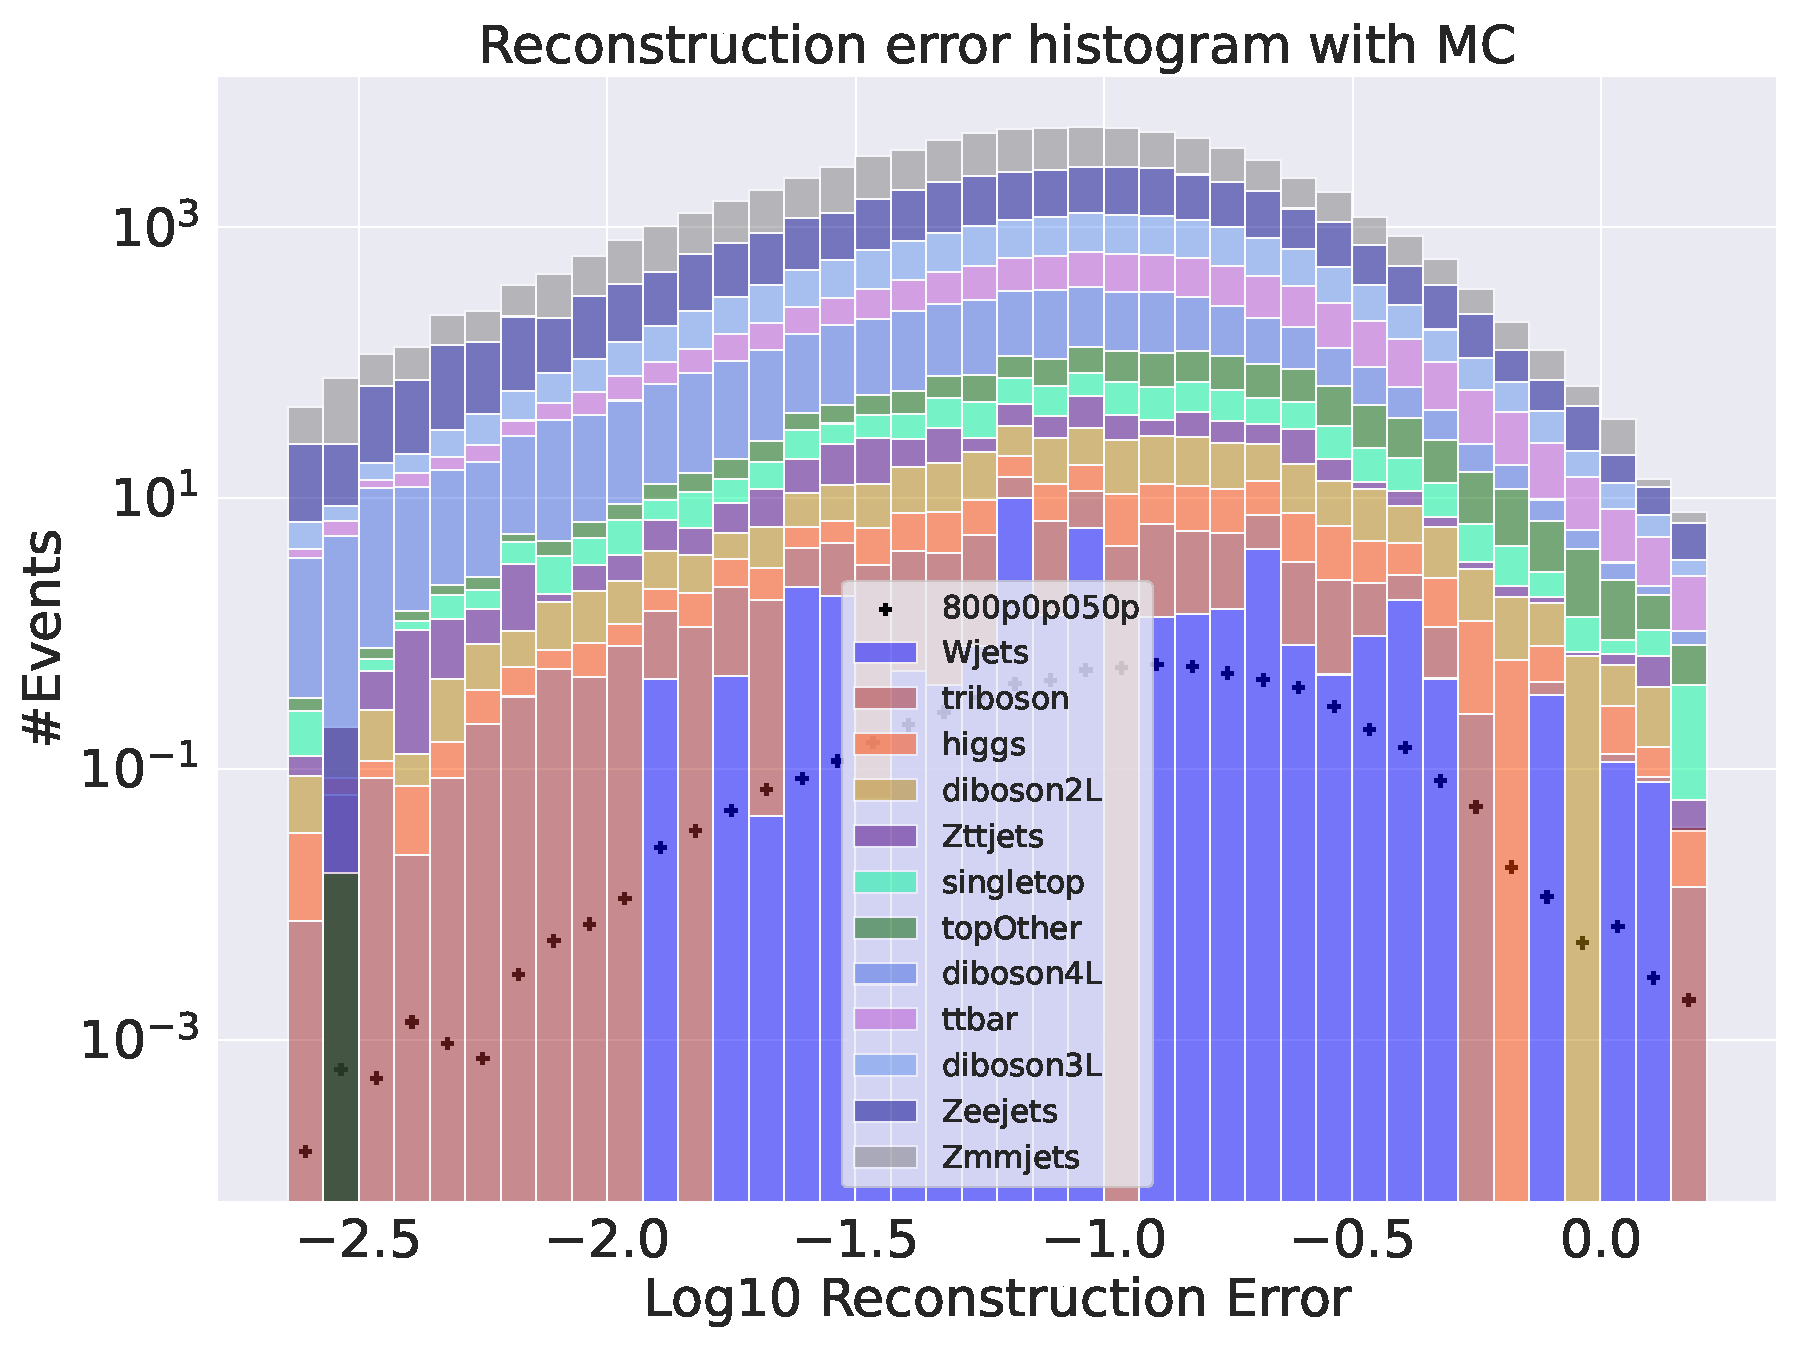
\includegraphics[width=\textwidth]{Figures/VAE_testing/small/3lep/b_data_recon_big_rm3_feats_sig_800p0p050p.pdf}
        \caption{ }
        \label{fig:VAE_3lep_small_800}
    \end{subfigure}
    \hfill
    \begin{subfigure}{.45\textwidth}
        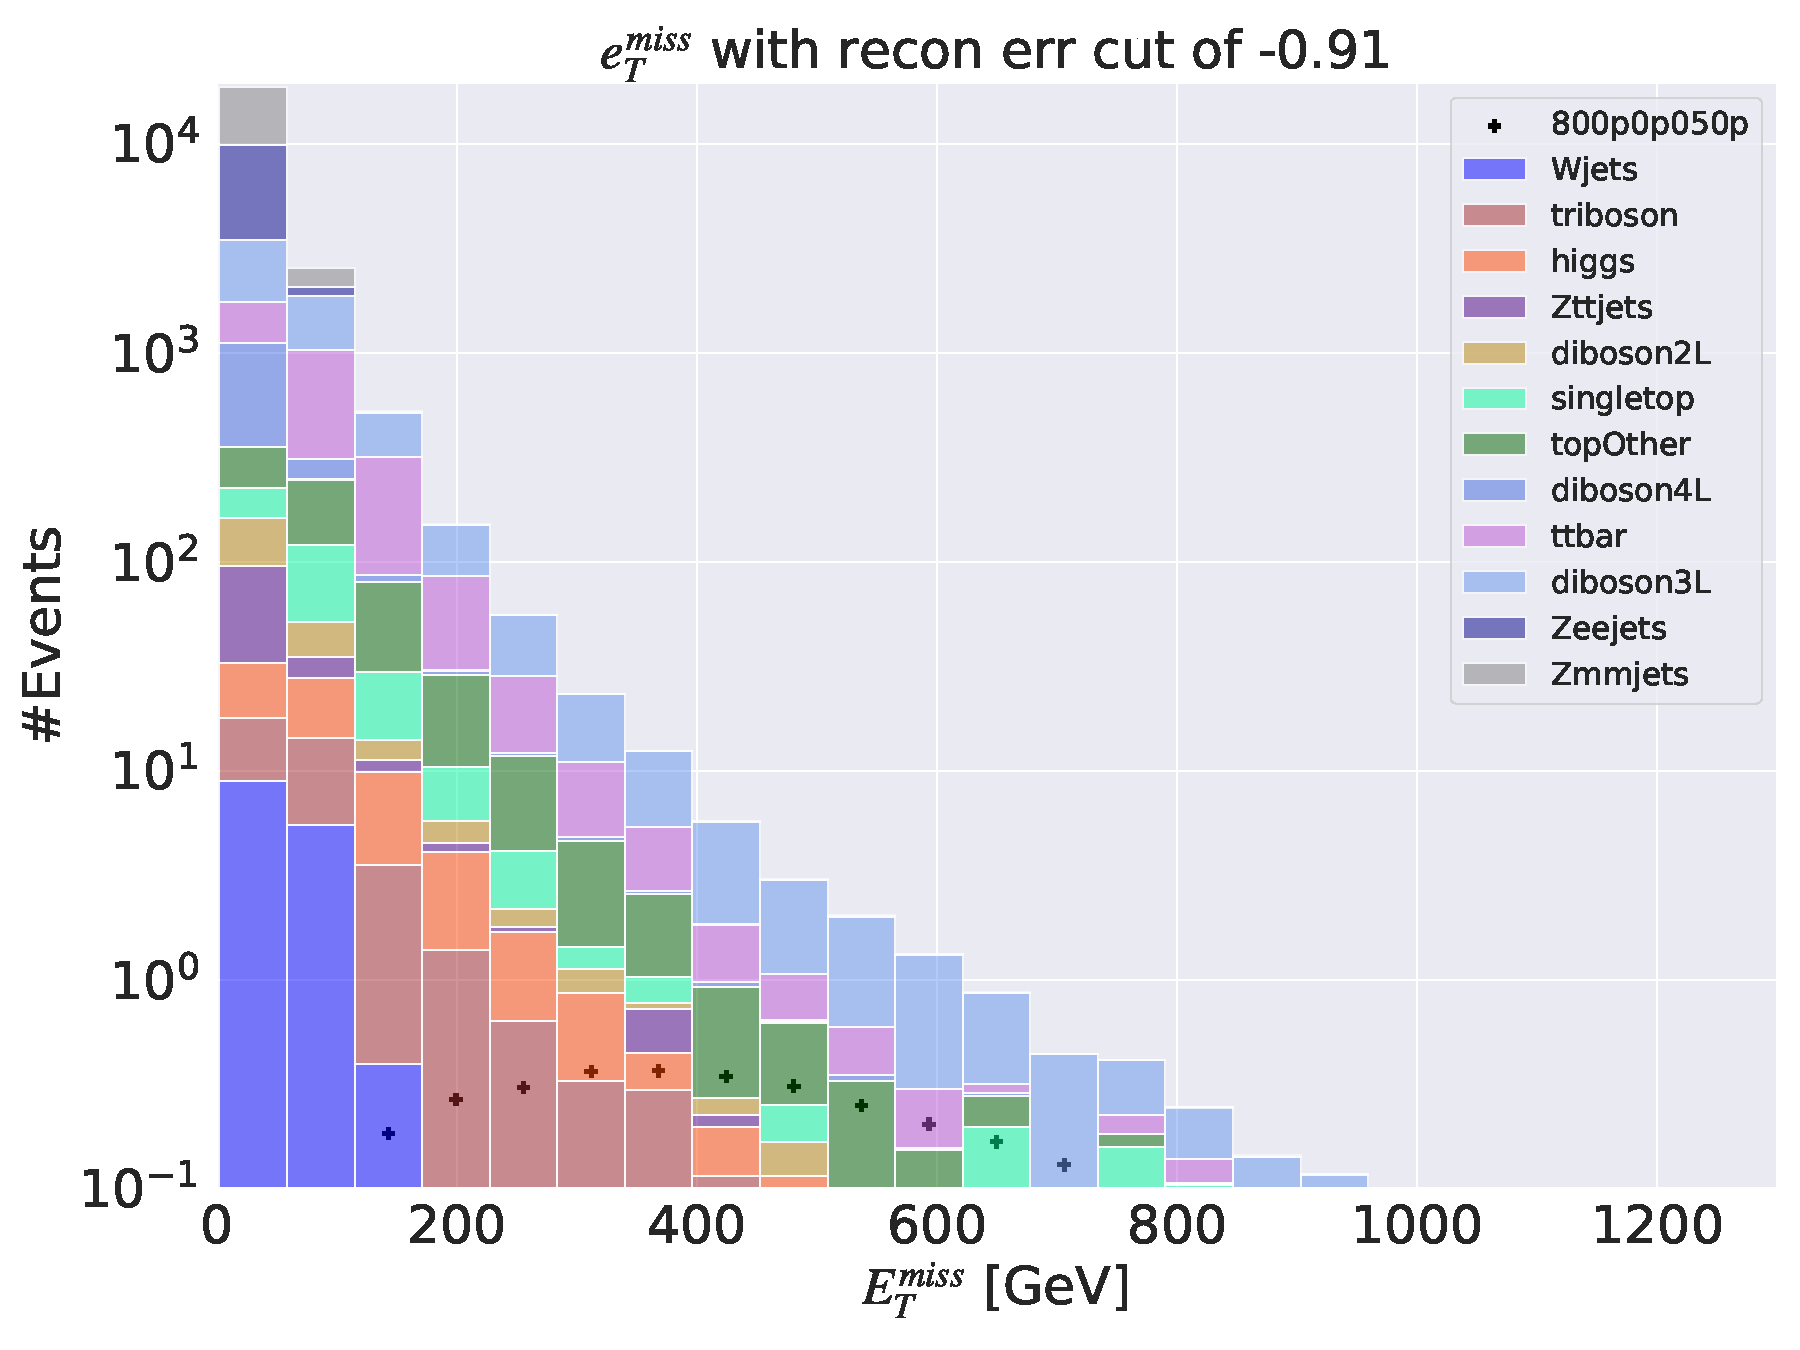
\includegraphics[width=\textwidth]{Figures/VAE_testing/small/3lep/b_data_recon_big_rm3_feats_sig_800p0p050p_etmiss_recon_errcut_-0.91.pdf}
        \caption{}
        \label{fig:VAE_3lep_small_etmiss_800}
    \end{subfigure}
    \hfill
    \begin{subfigure}{.45\textwidth}
        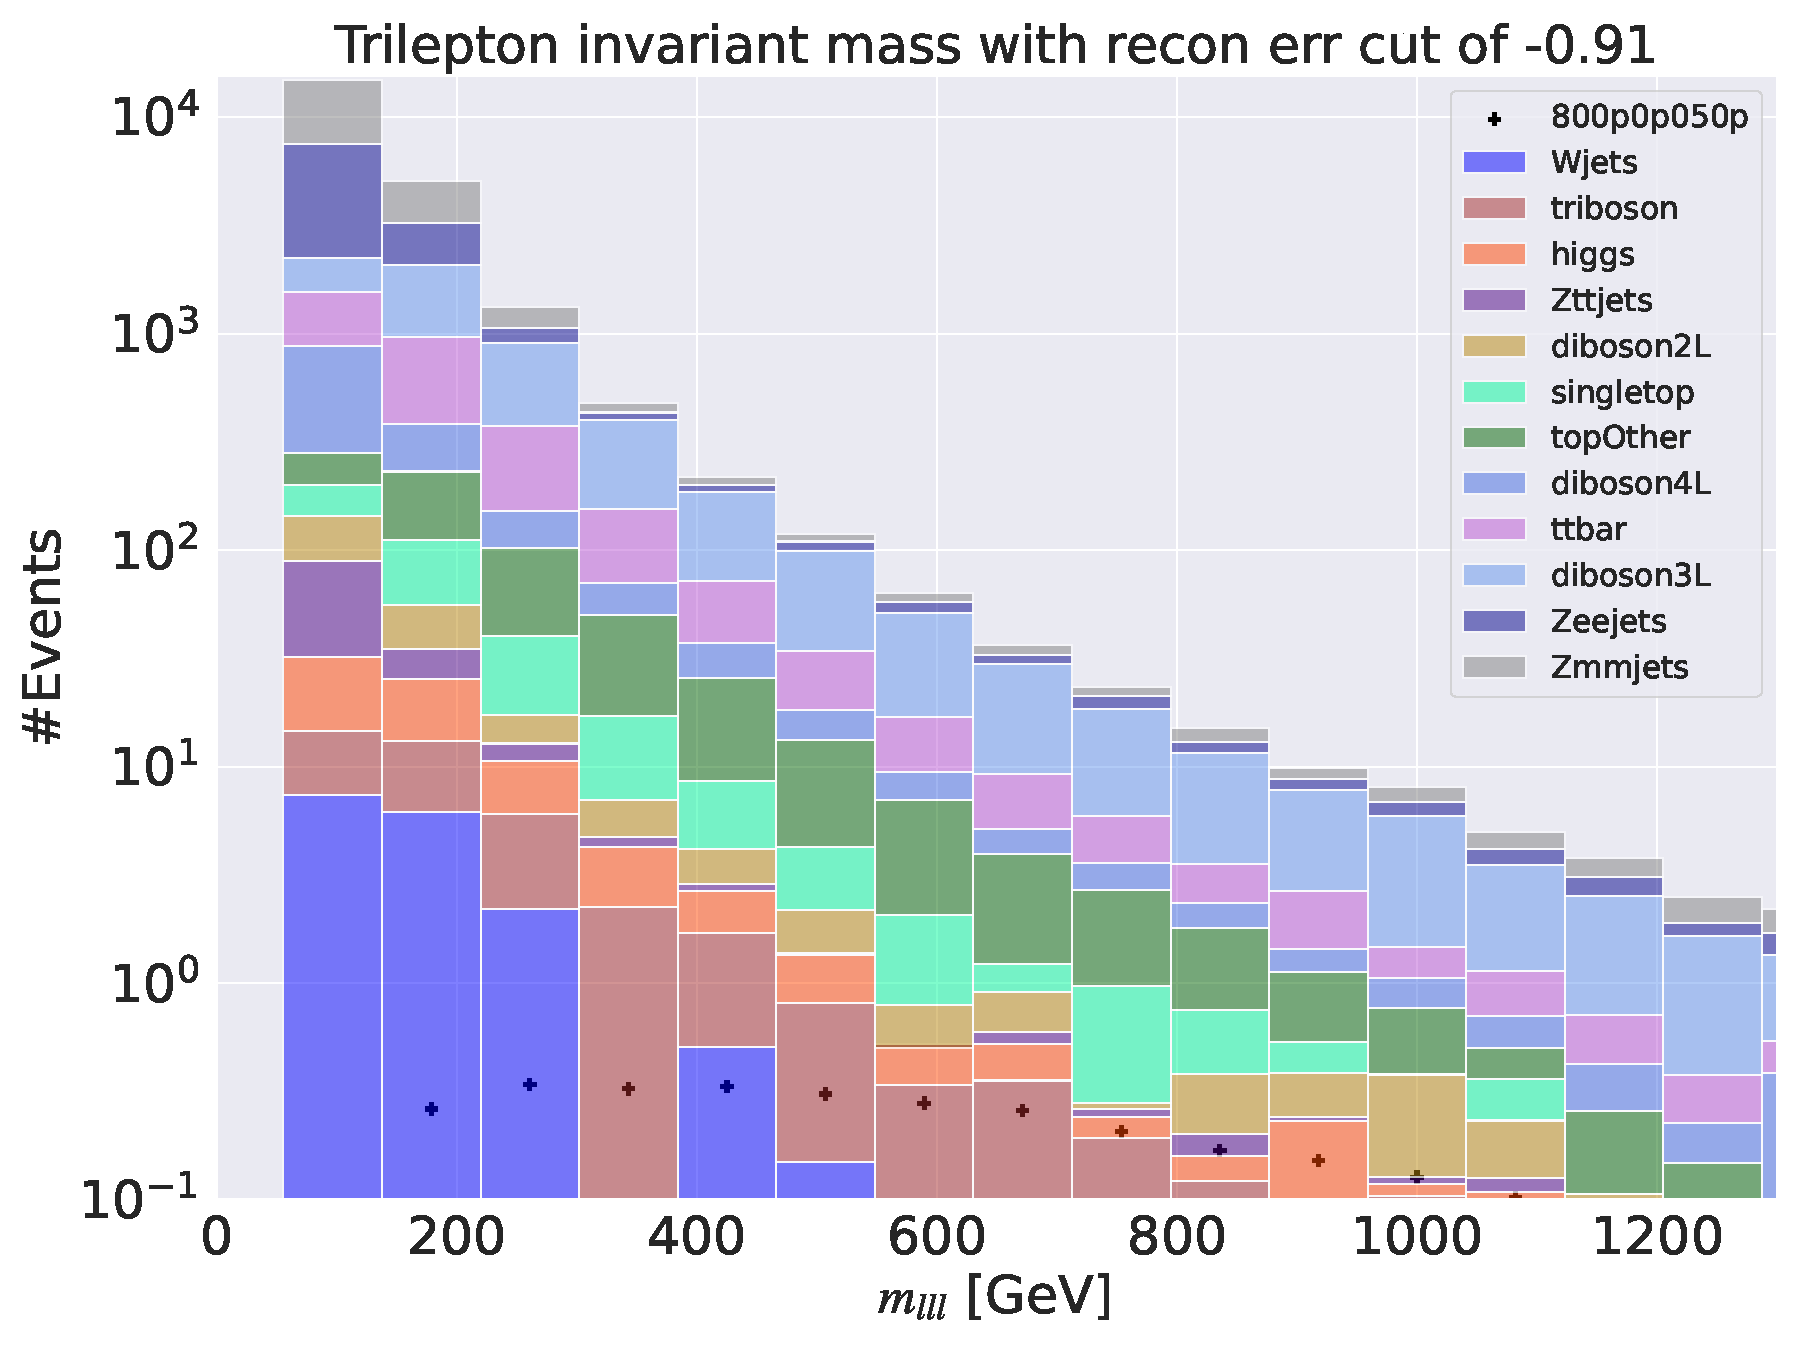
\includegraphics[width=\textwidth]{Figures/VAE_testing/small/3lep/b_data_recon_big_rm3_feats_sig_800p0p050p_mlll_recon_errcut_-0.91.pdf}
        \caption{}
        \label{fig:VAE_3lep_small_mlll_800}
    \end{subfigure}
    \hfill   
    \begin{subfigure}{.45\textwidth}
        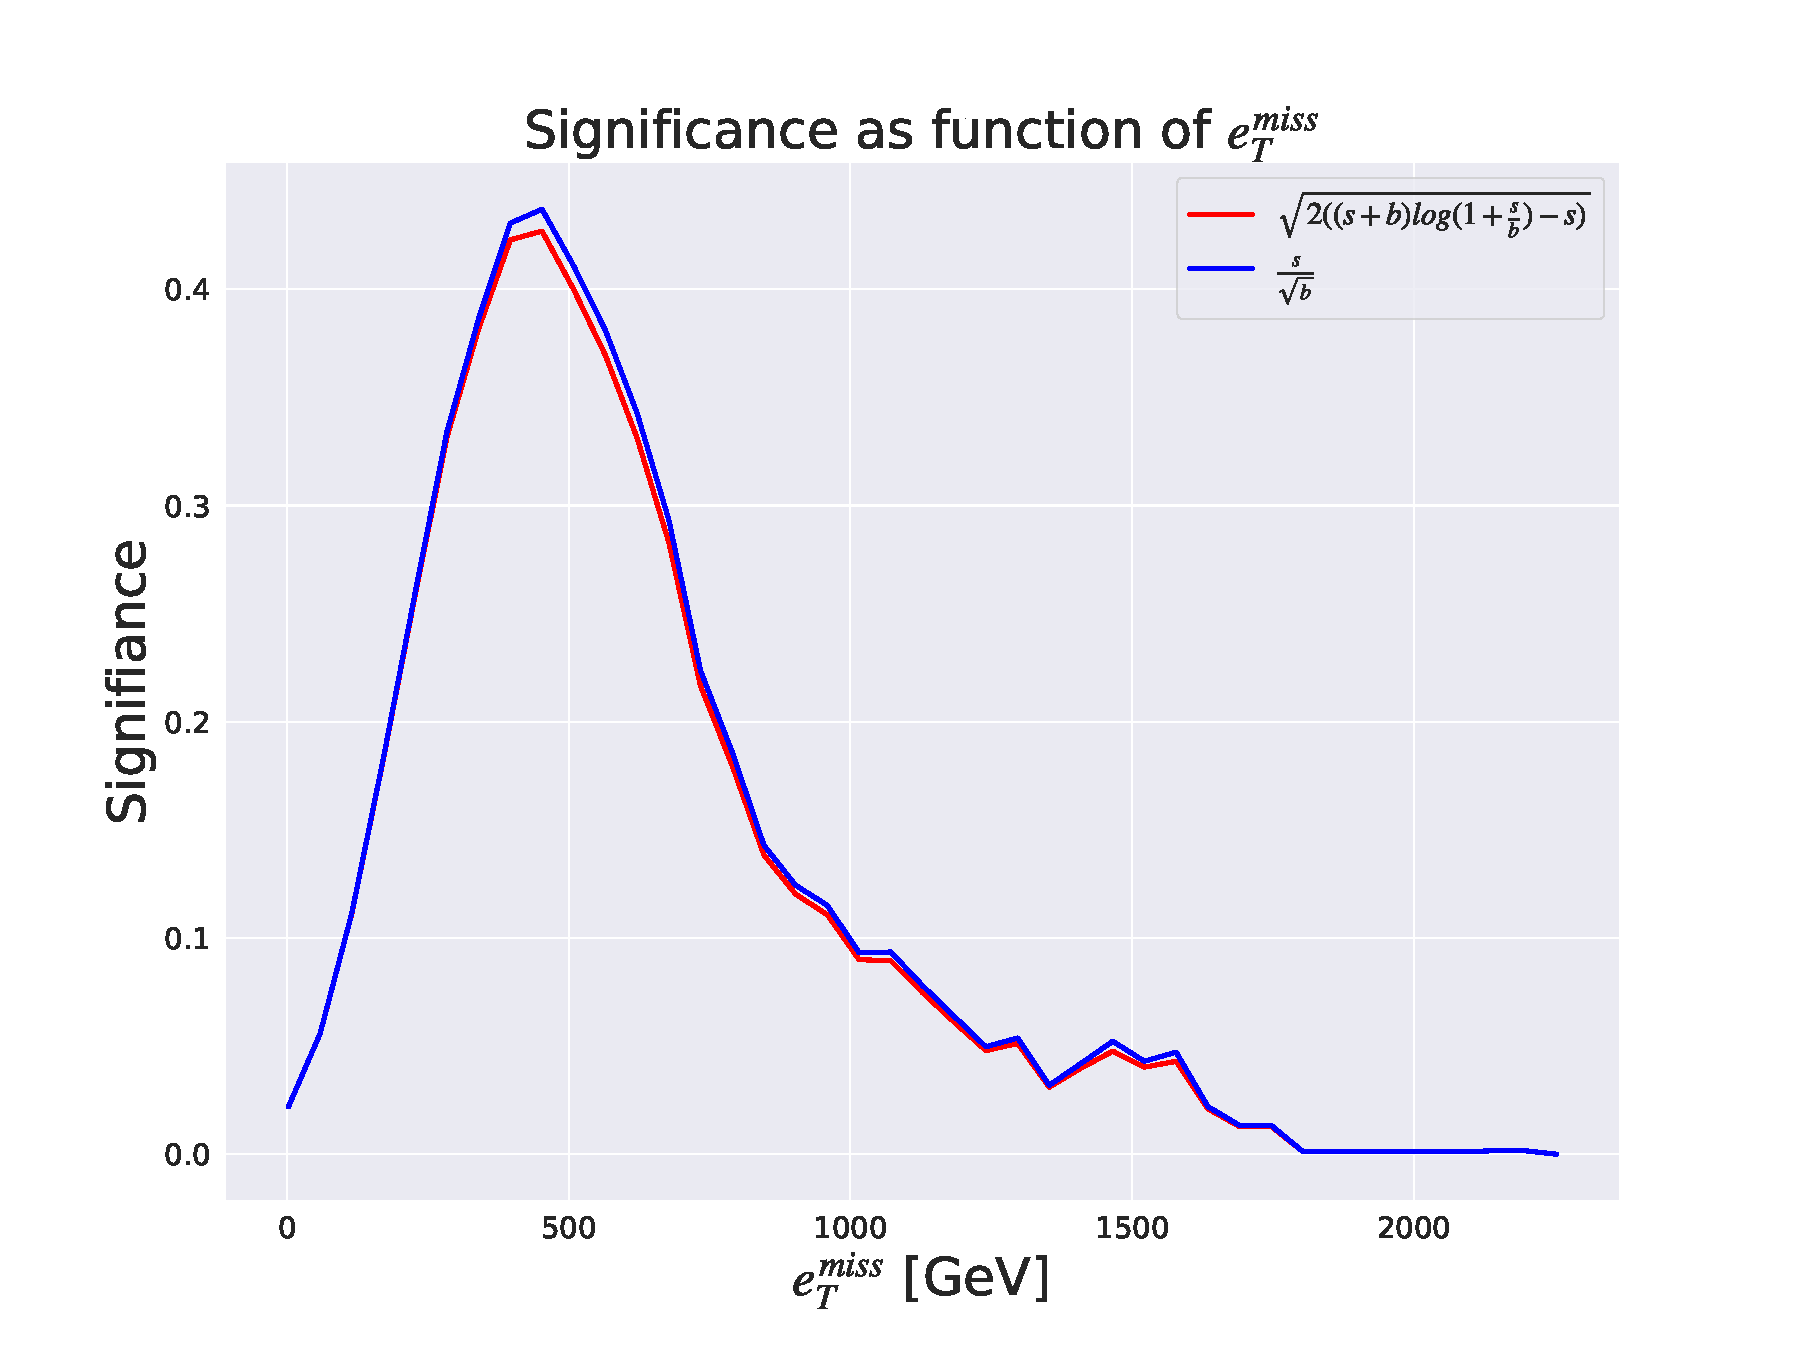
\includegraphics[width=\textwidth]{Figures/VAE_testing/small/3lep/significance_etmiss_800p0p050p_-0.9142561918890106.pdf}
        \caption{}
        \label{ffig:VAE_3lep_small_signi_800}
    \end{subfigure}
    \hfill      
    \caption[3lep shallow network | $800p50$]{Reconstruction error, $e_T^{miss}$ signal region, $m_{lll}$ signal region and significance as function of 
    $e_T^{miss}$ for the shallow regular autoencoder. Here the SUSY $450p300$ model is used.}
    \label{fig:VAE_3lep_small_rec_sig_signi_800}
\end{figure}



In figure REF we have the reconstruction error distributions for both SUSY signals from 
the shallow and deep variational autoencoder. Here we observe that the the variational autoencoder seems to struggle with 
differentiating betwwen background and signal, having the two distributions laying on top of each other. There is however a 
slight difference in the shape of the distributions from the shallow and deep network. The shallow has a more narrow 
and slightly more left leaning shale, where as the deep network has a slightly more broad distribution shifted a bit 
to the right. \par 
In the figures below we have the $e_T^{miss}$ distributions in one of the three signal regions created.




